%%%%%%%%%%%%%%%%%%%%%%%%%%%%%%%%%%%%%%%%%%%%%%%%%%%%%%%%%%%%%%%%%%%%%
%% This is a (brief) model paper using the achemso class
%% The document class accepts keyval options, which should include
%% the target journal and optionally the manuscript type. 
%%%%%%%%%%%%%%%%%%%%%%%%%%%%%%%%%%%%%%%%%%%%%%%%%%%%%%%%%%%%%%%%%%%%%
\documentclass[journal=jacsat,manuscript=article]{achemso}
\SectionNumbersOn
%\usepackage[letterpaper,left=0.5in,right=0.5in,top=1.0in,bottom=1.0in]{geometry}

%%%%%%%%%%%%%%%%%%%%%%%%%%%%%%%%%%%%%%%%%%%%%%%%%%%%%%%%%%%%%%%%%%%%%
%% Place any additional packages needed here.  Only include packages
%% which are essential, to avoid problems later. Do NOT use any
%% packages which require e-TeX (for example etoolbox): the e-TeX
%% extensions are not currently available on the ACS conversion
%% servers. 
%%%%%%%%%%%%%%%%%%%%%%%%%%%%%%%%%%%%%%%%%%%%%%%%%%%%%%%%%%%%%%%%%%%%%
\usepackage[version=3]{mhchem} % Formula subscripts using \ce{}
\usepackage{siunitx} % generating degrees Celsius in the document 
\usepackage{color}
\usepackage{soul} % allows highlighting text 
\usepackage{makecell}
\usepackage{booktabs}
\usepackage{amsmath}
\usepackage{amssymb}
\usepackage{todonotes}
\usepackage{gensymb}
\usepackage{verbatim}
\usepackage{hyperref}
\hypersetup{
    colorlinks=true,
    citecolor= red,
    linkcolor=blue,
    urlcolor=blue, 
    breaklinks=true
}
\usepackage{ulem}
\usepackage{float}

% Packages from the old SI section 
\usepackage{breakcites}
%\usepackage{caption}
\usepackage{float}
\usepackage[hang]{subfigure}
\usepackage{overpic}
\usepackage{listings}
\usepackage[super]{nth}
\usepackage{multicol}
\linespread{1.15}

\renewcommand{\thefigure}{S\arabic{figure}}
\renewcommand{\theequation}{S\arabic{equation}}
\renewcommand{\thesection}{S\arabic{section}}
\renewcommand{\thetable}{S\arabic{table}}

%%%%%%%%%%%%%%%%%%%%%%%%%%%%%%%%%%%%%%%%%%%%%%%%%%%%%%%%%%%%%%%%%%%%%
%% If issues arise when submitting your manuscript, you may want to
%% un-comment the next line.  This provides information on the
%% version of every file you have used.
%%%%%%%%%%%%%%%%%%%%%%%%%%%%%%%%%%%%%%%%%%%%%%%%%%%%%%%%%%%%%%%%%%%%%
%%\listfiles

%%%%%%%%%%%%%%%%%%%%%%%%%%%%%%%%%%%%%%%%%%%%%%%%%%%%%%%%%%%%%%%%%%%%%
%% Place any additional macros here.  Please use \newcommand* where
%% possible, and avoid layout-changing macros (which are not used
%% when typesetting).
%%%%%%%%%%%%%%%%%%%%%%%%%%%%%%%%%%%%%%%%%%%%%%%%%%%%%%%%%%%%%%%%%%%%%
\newcommand*\mycommand[1]{\texttt{\emph{#1}}}
\DeclareRobustCommand
  \Compactcdots{\mathinner{\cdotp\mkern-2mu\cdotp\mkern-2mu\cdotp}}

%%%%%%%%%%%%%%%%%%%%%%%%%%%%%%%%%%%%%%%%%%%%%%%%%%%%%%%%%%%%%%%%%%%%%
%% Meta-data block
%% ---------------
%% Each author should be given as a separate \author command.
%%
%% Corresponding authors should have an e-mail given after the author
%% name as an \email command. Phone and fax numbers can be given
%% using \phone and \fax, respectively; this information is optional.
%%
%% The affiliation of authors is given after the authors; each
%% \affiliation command applies to all preceding authors not already
%% assigned an affiliation.
%%
%% The affiliation takes an option argument for the short name.  This
%% will typically be something like "University of Somewhere".
%%
%% The \altaffiliation macro should be used for new address, etc.
%% On the other hand, \alsoaffiliation is used on a per author basis
%% when authors are associated with multiple institutions.
%%%%%%%%%%%%%%%%%%%%%%%%%%%%%%%%%%%%%%%%%%%%%%%%%%%%%%%%%%%%%%%%%%%%%
\author{Stephen P. Vicchio}
\affiliation[Clemson University]
{Department of Chemical and Biomolecular Engineering, Clemson University, Clemson, SC}
\author{Zhihengyu Chen}
\affiliation[Stony Brook University]
{Department of Chemistry, Stony Brook University, Stony Brook, NY}
\author{Karena W. Chapman}
\email{karena.chapman@stonybrook.edu}
\affiliation[Stony Brook University]
{Department of Chemistry, Stony Brook University, Stony Brook, NY}
\author{Rachel B. Getman}
\email{rgetman@clemson.edu}
\affiliation[Clemson University]
{Department of Chemical and Biomolecular Engineering, Clemson University, Clemson, SC}

%%%%%%%%%%%%%%%%%%%%%%%%%%%%%%%%%%%%%%%%%%%%%%%%%%%%%%%%%%%%%%%%%%%%%
%% The document title should be given as usual. Some journals require
%% a running title from the author: this should be supplied as an
%% optional argument to \title.
%%%%%%%%%%%%%%%%%%%%%%%%%%%%%%%%%%%%%%%%%%%%%%%%%%%%%%%%%%%%%%%%%%%%%
\title[manuscript]{
Supporting Information: \\
Computational and Experimental Characterization of the Ligand Environment of a \ce{Ni}-Oxo Catalyst Cluster Supported in the Metal-Organic Framework NU-1000}

%%%%%%%%%%%%%%%%%%%%%%%%%%%%%%%%%%%%%%%%%%%%%%%%%%%%%%%%%%%%%%%%%%%%%
%% Some journals require a list of abbreviations or keywords to be
%% supplied. These should be set up here, and will be printed after
%% the title and author information, if needed.
%%%%%%%%%%%%%%%%%%%%%%%%%%%%%%%%%%%%%%%%%%%%%%%%%%%%%%%%%%%%%%%%%%%%%
\abbreviations{IR,NMR,UV}
\keywords{American Chemical Society, \LaTeX}

%%%%%%%%%%%%%%%%%%%%%%%%%%%%%%%%%%%%%%%%%%%%%%%%%%%%%%%%%%%%%%%%%%%%%
%% The manuscript does not need to include \maketitle, which is
%% executed automatically.
%%%%%%%%%%%%%%%%%%%%%%%%%%%%%%%%%%%%%%%%%%%%%%%%%%%%%%%%%%%%%%%%%%%%%
\begin{document}

%%%%%%%%%%%%%%%%%%%%%%%%%%%%%%%%%%%%%%%%%%%%%%%%%%%%%%%%%%%%%%%%%%%%%
%% The "tocentry" environment can be used to create an entry for the
%% graphical table of contents. It is given here as some journals
%% require that it is printed as part of the abstract page. It will
%% be automatically moved as appropriate.
%%%%%%%%%%%%%%%%%%%%%%%%%%%%%%%%%%%%%%%%%%%%%%%%%%%%%%%%%%%%%%%%%%%%%
%\begin{tocentry}
%
%Some journals require a graphical entry for the Table of Contents.
%This should be laid out ``print ready'' so that the sizing of the
%text is correct.
%
%Inside the \texttt{tocentry} environment, the font used is %Helvetica
%8\,pt, as required by \emph{Journal of the American Chemical
%Society}.
%
%The surrounding frame is 9\,cm by 3.5\,cm, which is the maximum
%permitted for  \emph{Journal of the American Chemical Society}
%graphical table of content entries. The box will not resize if the
%content is too big: instead it will overflow the edge of the box.
%
%This box and the associated title will always be printed on a
%separate page at the end of the document.
%
%\end{tocentry}

%%%%%%%%%%%%%%%%%%%%%%%%%%%%%%%%%%%%%%%%%%%%%%%%%%%%%%%%%%%%%%%%%%%%%
%% The abstract environment will automatically gobble the contents
%% if an abstract is not used by the target journal.
%%%%%%%%%%%%%%%%%%%%%%%%%%%%%%%%%%%%%%%%%%%%%%%%%%%%%%%%%%%%%%%%%%%%%

%%%%%%%%%%%%%%%%%%%%%%%%%%%%%%%%%%%%%%%%%%%%%%%%%%%%%%%%%%%%%%%%%%%%%
%% Start the main part of the manuscript here.
%%%%%%%%%%%%%%%%%%%%%%%%%%%%%%%%%%%%%%%%%%%%%%%%%%%%%%%%%%%%%%%%%%%%%

%%%%%%%%%%%%%%%%%%%%%%%%%%%%%%%%%%%%%%%%%%%%%%%%%%%%%%%%%%%%%%%%%%%%%
%% Start the table of content here
%%%%%%%%%%%%%%%%%%%%%%%%%%%%%%%%%%%%%%%%%%%%%%%%%%%%%%%%%%%%%%%%%%%%%
\newpage
\tableofcontents


%%%%%%%%%%%%%%%%%%%%%%%%%%%%%%%%%%%%%%%%%%%%%%%%%%%%%%%%%%%%%%%%%%%%%
%% Computational Methodology
%%%%%%%%%%%%%%%%%%%%%%%%%%%%%%%%%%%%%%%%%%%%%%%%%%%%%%%%%%%%%%%%%%%%%
\newpage
\section{Computational Methodology}
\subsection{Schematic for \textit{ab initio} thermodynamic analysis}
    \begin{figure}[H]
        \centering
        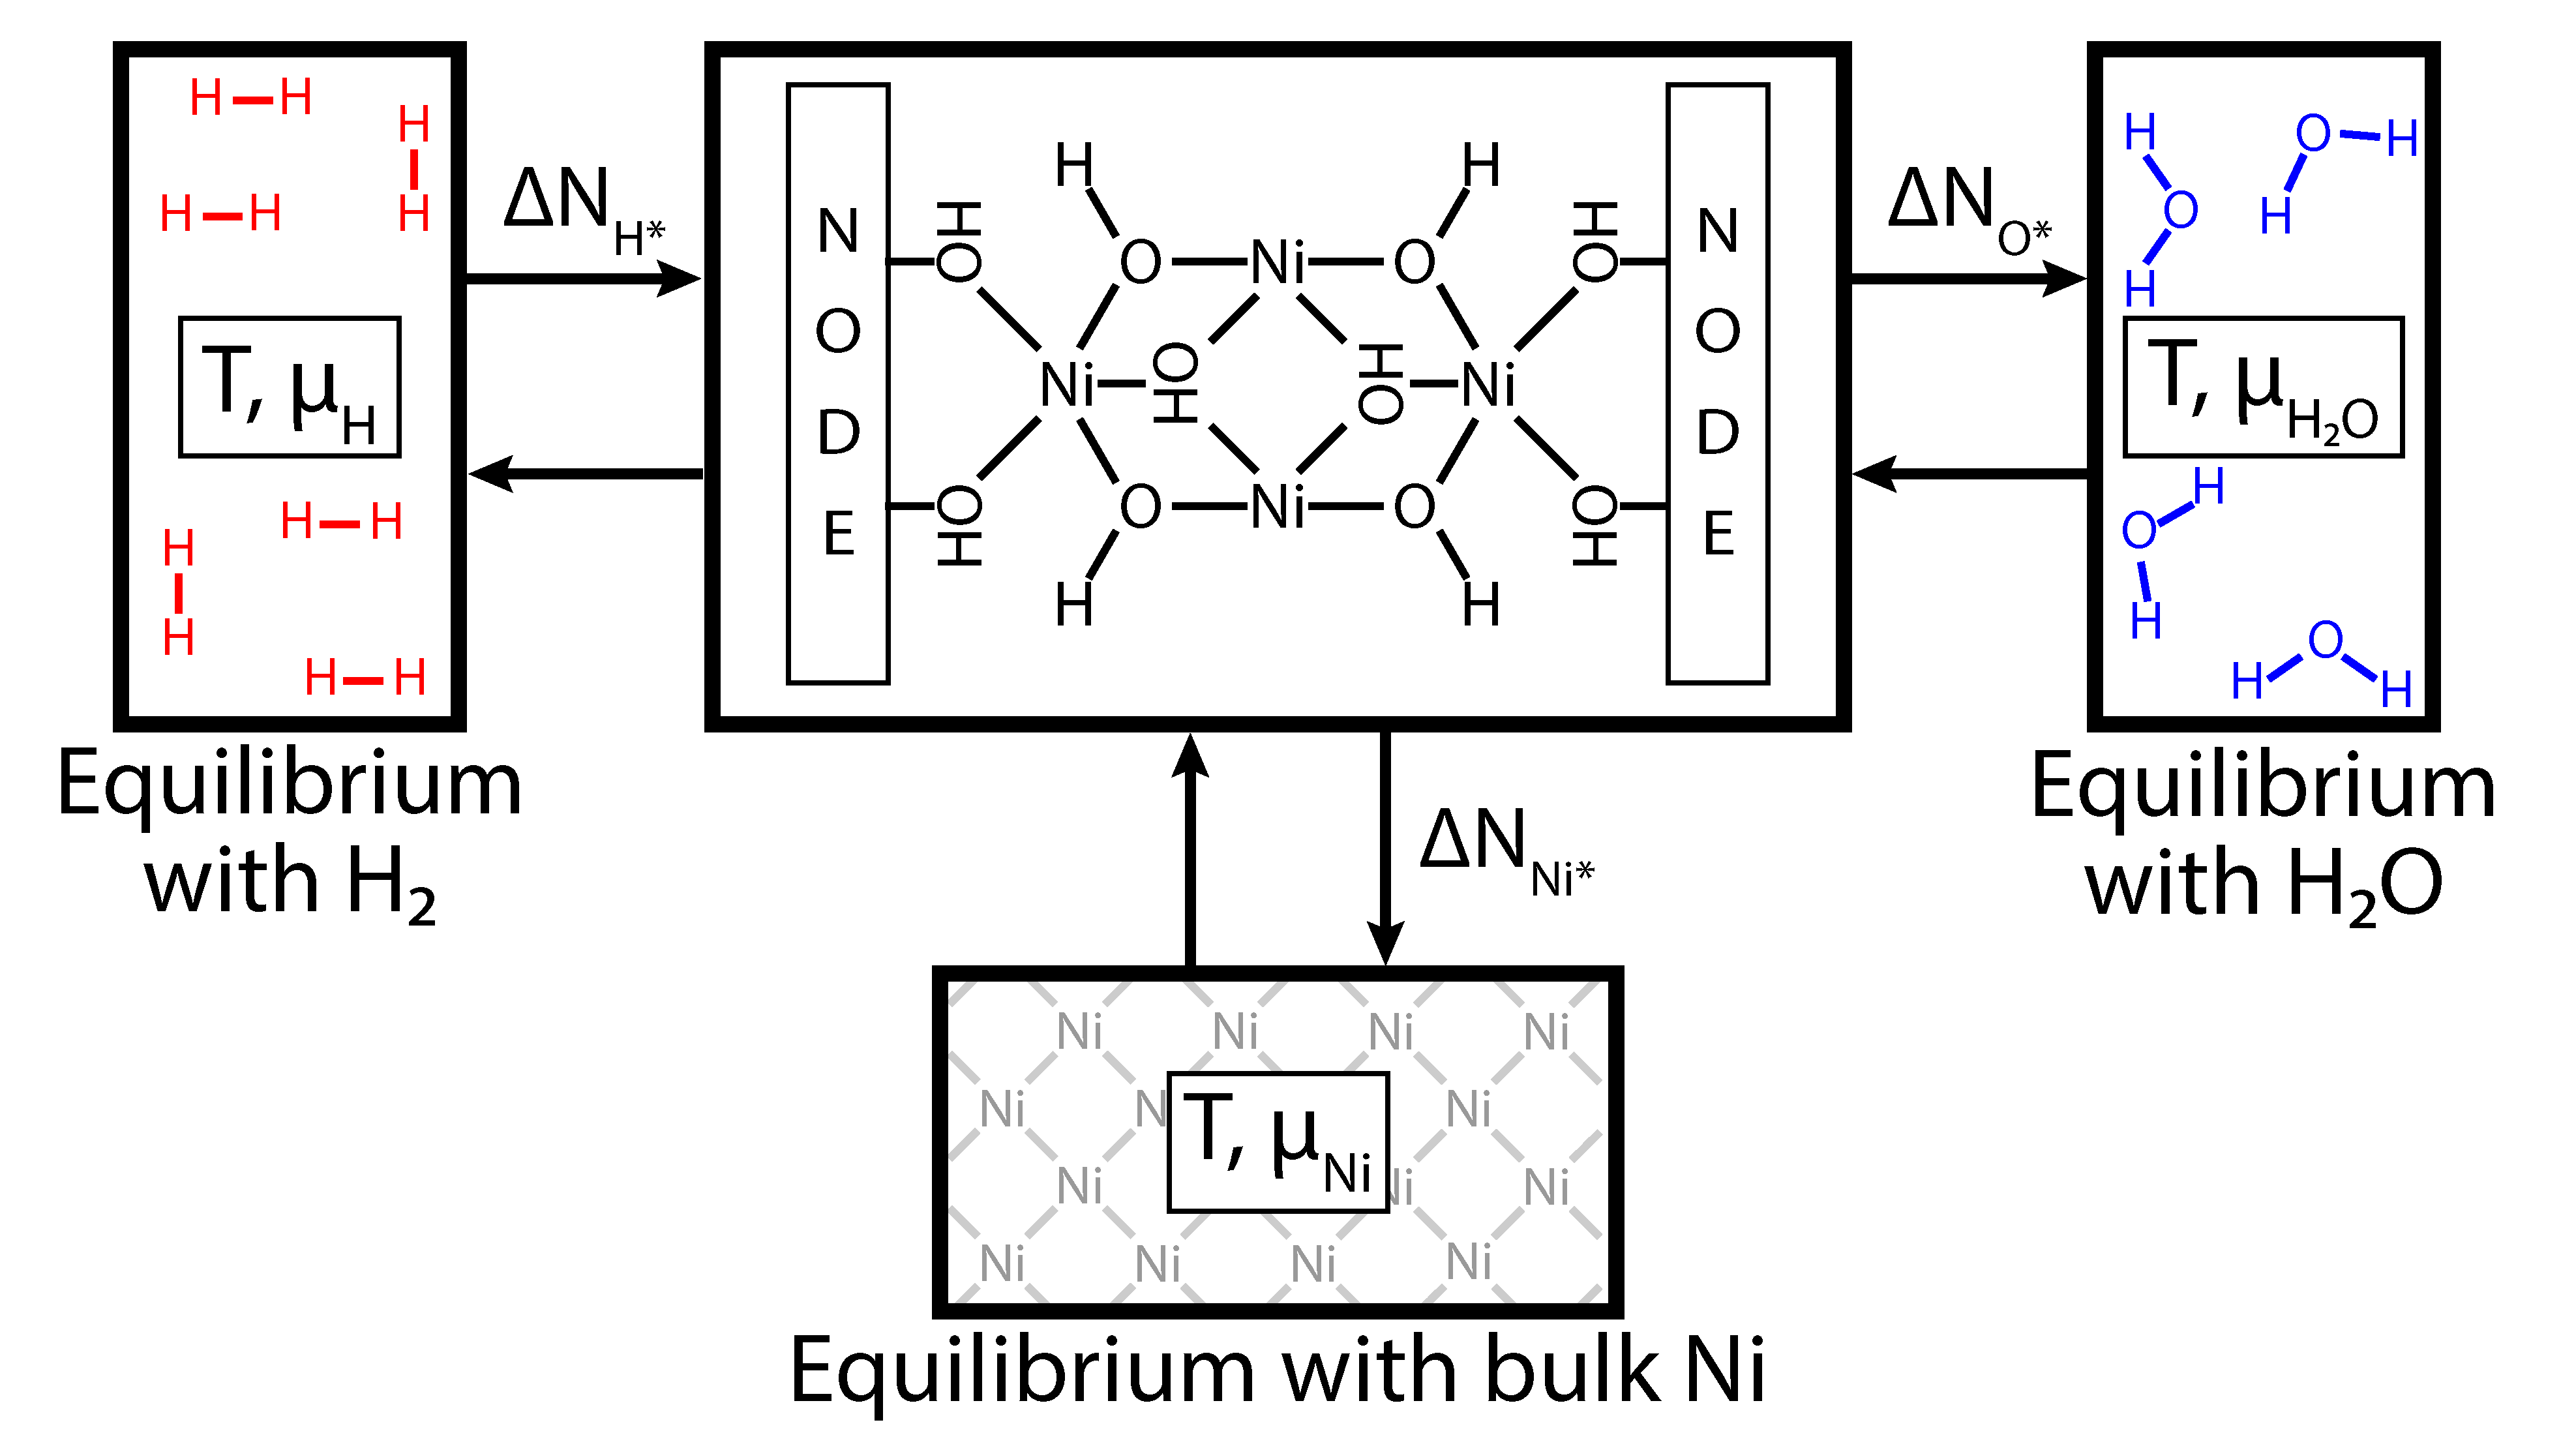
\includegraphics[width=0.80\textwidth]{zi-images/04-SI-images/SI-FPT-schematic-full.png}
        \caption{Diagram showing the assumed equilibria necessary to transform with \ce{H}, \ce{OH}, \ce{Ni} for the \textit{ab initio} thermodynamic analysis method. The assume assumed equilibria capture the operating conditions influences on the stability of the \ce{Ni} ion cluster.}
        \label{fig:SI-FPT-process-diagram}
    \end{figure}


    Figure~\ref{fig:SI-FPT-process-diagram} shows a schematic for \textit{ab initio} thermodynamic analysis,\cite{Reuter2003, Reuter2004, Grundner2015, Paolucci2016, Li2016, Getman2008, Mandal2020, Zuo2016, Tang2019} which is used to evaluate the stability of a \ce{Ni4}-cluster supported on NU-1000. We assume the \ce{Ni} ion cluster is in equilibrium with three different reservoirs, which allows for transformations with respect to \ce{H}, \ce{O}, and \ce{Ni}. Equilibrium with the bulk \ce{Ni} reservoir is turned off by assuming $\Delta N_{\ce{Ni}} = 0$, implying that the number of \ce{Ni} ions is fixed at four. We derive expressions relating the chemical potentials for each transformed species to their respective bulk reservoirs.   

%%%%%%%%%%%%%%%%%%%%%%%%%%%%%%%%%%%%%%%%%%%%%%%%%%%%%%%%%%%%%%%%%%%%%
%% Free Energy Expression
%%%%%%%%%%%%%%%%%%%%%%%%%%%%%%%%%%%%%%%%%%%%%%%%%%%%%%%%%%%%%%%%%%%%%
\newpage
\subsection{Deriving the free energy expressions}
We transform the free energy from a fixed number of atoms to a fixed chemical potential to account for the compositional variation of different activated clusters (Eq.~\ref{eq:transformation1}) using Legendre transforms:\cite{Alberty1997}
\begin{equation}
    F^{(0)}(V,T,N_{\text{H}},N_{\text{O}},N_{\text{Ni}}) \rightarrow 
    F^{(2)}(V,T,\mu_{\text{H}}, \mu_{\text{O}}, N_{\text{Ni}})    \rightarrow F^{(3)}(V,T,\mu_{\text{H}},\mu_{\text{O}},\mu_{\text{Ni}})
    \label{eq:transformation1}
\end{equation}
where $F$ is the Helmholtz free energy, $V$ is volume, $T$ is temperature, $\mu$ is chemical potential, and $N$ is the number of \ce{O}, \ce{H}, and \ce{Ni} atoms. The (2) superscript on $F^{(2)}$ indicates the second Legendre transform of $F^{(0)}$ (i.e., of $N_{\ce{H}}$ and $N_{\ce{O}}$ to $\mu_{\ce{H}}$ and $\mu_{\ce{O}}$, respectively). Additionally, the (3) superscript on $F^{(3)}$ indicates the Legendre transform of $F^{(2)}$ from $N_{\ce{Ni}}$ to $\mu_{\ce{Ni}}$. We write the transformed free energy expression for $F^{(2)}$ as Eq.~\ref{eq:free-energy-ind} and $F^{(3)}$ as Eq.~\ref{eq:free-energy-ind-Ni}. 
\begin{equation}
    \begin{split}
        F^{(2)}(V,T,\mu_{\text{H}},\mu_{\text{O}},N_{\text{Ni}}) =  F^{(0)}(V,T,N_{\text{H}},N_{\text{O}},N_{\text{Ni}}) - (\mu_{\text{H}})(N_{\text{H}}) - (\mu_{\text{O}})(N_{\text{O}})  \\ 
    \end{split}
    \label{eq:free-energy-ind}
\end{equation}
\begin{equation}
    \begin{split}
        F^{(3)}(V,T,\mu_{\text{H}},\mu_{\text{O}},\mu_{\text{Ni}}) = F^{(2)}(V,T,\mu_{\text{H}},\mu_{\text{O}},N_{\text{Ni}}) - (\mu_{\text{Ni}})(N_{\text{Ni}}) \\ 
    \end{split}
    \label{eq:free-energy-ind-Ni}
\end{equation}

The final transformed free energy expression ($\Delta F^{(2)}$) is computed relative to the reference structure, \ce{Ni4(OH)6.4H2O} (green), as shown in Figure~\ref{fig:SI-dPDF-green}. We write the transformed free energy expression for $\Delta F^{(2)}$ as Eq.~\ref{eq:free-energy-trans}: 
\begin{equation}
    \begin{split}
        \Delta F^{(2)}(V,T,\mu_{\text{H}},\mu_{\text{O}},N_{\text{Ni}})  
        & = \Delta F^{(0)}(V,T,N_{\text{H}},N_{\text{O}},N_{\text{Ni}}) - (\mu_{\text{H}})(\Delta N_{\text{H}}) 
        - (\mu_{\text{O}})(\Delta N_{\text{O}})  \\ 
    \end{split}
    \label{eq:free-energy-trans}
\end{equation}
where $\Delta N_{\text{H}}$ and $\Delta N_{\text{O}}$ are computed by taking the difference in the number of \ce{O} and \ce{H} atoms of the cluster relative to the reference structure. A similar expression is constructed for $F^{(3)}$ (Eq.~\ref{eq:free-energy-trans-Ni}) when looking at variable \ce{Ni} ion content:
\begin{equation}
    \begin{split}
        \Delta F^{(3)}(V,T,\mu_{\text{H}},\mu_{\text{O}},\mu_{\text{Ni}})  
        = \Delta F^{(2)}(V,T,\mu_{\text{H}},\mu_{\text{O}},N_{\text{Ni}}) - (\mu_{\text{Ni}})(\Delta N_{\text{Ni}}) \\ 
    \end{split}
    \label{eq:free-energy-trans-Ni}
\end{equation}
where $\Delta N_{\text{Ni}}$ is also computed by taking the difference in the number of \ce{Ni} atoms of the cluster relative to the reference structure. 

%%%%%%%%%%%%%%%%%%%%%%%%%%%%%%%%%%%%%%%%%%%%%%%%%%%%%%%%%%%%%%%%%%%%%
%% Equilibrium Expressions
%%%%%%%%%%%%%%%%%%%%%%%%%%%%%%%%%%%%%%%%%%%%%%%%%%%%%%%%%%%%%%%%%%%%%
\newpage
\subsection{Equilibrium expressions for chemical potential terms}
Eq.~\ref{eq:free-energy-trans} computes the free energy as a function of both \ce{H} and \ce{O} chemical potentials ($\mu_{\text{H}}$ and $\mu_{\text{O}}$). During \textit{ab initio} thermodynamic analysis, these chemical potentials are varied to study their influence on the free energy. As described in Fig.~\ref{fig:SI-FPT-process-diagram}, the cluster is assumed to be in equilibrium with \ce{H2} and \ce{H2O} reservoirs; we relate reservoir chemical potentials to the chemical potentials of the cluster atoms, \ce{H} and \ce{O} (from Eq.~\ref{eq:free-energy-trans}). 

For \ce{H} on the \ce{Ni4}-cluster, the assumed equilibrium is with a reservoir of \ce{H2} gas:
\begin{equation}
    \ce{H} \ce{<=>} \frac{1}{2} \ce{H2}(g)  
\end{equation}
with the chemical potential terms related according to:
\begin{equation}
    \mu_{\ce{H}} = \frac{1}{2} \mu_{\ce{H2}}^{g}(T,P)
\end{equation}  
$\mu_{\ce{H2}}^{g}(T,P)$ is the gas phase reservoir chemical potential term, and is computed by  correcting the electronic energy (referenced at $T$=0 K) of an isolated molecule with the gas-phase free energy values at a specific temperature and pressure.\cite{Li2016} Eq.~\ref{H2-to-reaction-conditions} shows the correction. 
\begin{equation}
    \begin{split}
         \mu_{\ce{H2}}^{g}(T,P) &= E_{\ce{H2}}^{\text{DFT}} + E_{\ce{H2}}^{\text{ZPE}}+ \Delta \mu_{\ce{H2}}(T,P)  \\
    \end{split}
    \label{H2-to-reaction-conditions}
\end{equation}
In our analysis, $\Delta \mu_{\ce{H2}}(T,P)$ is an independent variable. By varying $\Delta \mu_{\ce{H2}}(T,P)$, we compute the free energy at different conditions, which generates the all phase diagrams and heat maps.

For \ce{O} on the \ce{Ni4}-cluster, the assumed equilibrium is with a reservoir of both \ce{H2O} and \ce{H2} gas:
\begin{equation}
    \ce{H2} + \ce{O} \ce{<=>} \ce{H2O}
\end{equation}
with the chemical potential terms related according to:
\begin{equation}
    \mu_{\ce{O}} = \mu_{\ce{H2O}}^{g}(T,P) - \mu_{\ce{H2}}^{g}(T,P)
\end{equation}
where $\mu_{\ce{H2O}}^{g}(T,P)$ is the gas phase reservoir chemical potential term. A similar expression to Eq.~\ref{H2-to-reaction-conditions} is constructed to relate the electronic energy (referenced at $T$=0 K) of an isolated molecule with the gas-phase free energy values (Eq.~\ref{H2O-to-reaction-conditions}). 
\begin{equation}
    \begin{split}
         \mu_{\ce{H2O}}^{g}(T,P) &= E_{\ce{H2O}}^{\text{DFT}} + E_{\ce{H2O}}^{\text{ZPE}} + \Delta \mu_{\ce{H2O}}(T,P)  \\
    \end{split}
    \label{H2O-to-reaction-conditions}
\end{equation}
Again, $\Delta \mu_{\ce{H2O}}(T,P)$ is another independent variable that is tunable in our analysis. Unlike \ce{H2}, the \ce{H2O} chemical potential is not known for these systems. During activation, the cluster is exposed to 3.5\% \ce{H2} in \ce{He} gas at $P$ = 1 bar and $T$ ranging from 50 \degree C to 200 \degree C.\cite{Li2016sintering} We can relate these conditions to an \ce{H2} chemical potential; however, water is not explicitly added to the system during activation or subsequent steps. We therefore vary the \ce{H2O} chemical potential by changing $\Delta \mu_{\ce{H2O}}(T,P)$ during \textit{ab initio} thermodynamic analysis. Phase diagrams are computed as a function of $\Delta \mu_{\ce{H2}}(T,P)$ and $\Delta \mu_{\ce{H2O}}(T,P)$.

\newpage
\subsection{Frequency Calculations}
We fix the organic linker and inorganic nodes, thereby only calculating only the \ce{Ni4}-cluster vibrational contributions to the free energy ($F^\text{vib}$). We ensure that the same atoms are fixed across all frequency calculations in order to correctly compare ($F^\text{vib}$). When constructing the vibrational partition function, all frequencies less than 50 cm\textsuperscript{-1} are replaced with 50 cm\textsuperscript{-1} to correct for the breakdown in the harmonic oscillator approximation for low frequency vibrational modes.\cite{Ribeiro2011} The partitions functions are computed in the pMuTT\cite{LYM2019106864} Python package to compute $E^\text{ZPE}$ and $F^\text{vib}$ for all structures. A sample input file for the CP2K frequency calculations is provided in the Supporting Information. The following expression is used to compute $F^{(0)}$ of each \ce{Ni4}-cluster structure: 
\begin{equation}
    \begin{split}
        F^{(0)} = E^{\text{DFT}} + E^\text{ZPE} + F^\text{vib}
    \end{split}
    \label{eq:free-energy-from-DFT}
\end{equation}


\newpage
\subsection{Deriving gas phase free energies values from empirical data}
Both $\Delta \mu_{\ce{H2}}(T,P)$ and $\Delta \mu_{\ce{H2O}}(T,P)$ written as a function of $T$ and $P$ is shown generically in Eq.~\ref{chemical_potential_ref}. The $\Delta \mu_{i}(T,P)$ term includes all temperature- and pressure- free energy contributions. 
\begin{equation}
        \Delta \mu_{i}(T,P) = \Delta \mu_{i}(T,P^{o}) + \Big[ RT \ln{ \frac{P}{P^{o}}} \Big]
    \label{chemical_potential_ref}
\end{equation}
where $\Delta \mu_{i}(T,P^{o})$ is the chemical potential of species $i$ referenced at $T$ is the temperature and $P^{o}$, and $R$ is gas constant. $\Delta \mu_{i}(T,P^{o})$ is computed using the NASA Polynomials\cite{Mcbride1993}, following a conversion from standard temperature to 0 K:
\begin{equation}
    \begin{split}
        \Delta G(T, P^{o}) &= [G(T,P^{o}) - G(T=298 K, P^{o})] - [G(T=10 K, P^{o}) - G(T=298 K, P^{o})] \\
        \Delta G(T, P^{o}) &= [G(T,P^{o})] - [G(T=10 K, P^{o})] 
    \end{split}
    \label{eq:pmutt-expression}
\end{equation} 
where $\Delta G(T, P^{o})$ is the free energy referenced at $T = 10$~K. The NASA Polynomial were extrapolated to be referenced to 0~K using pMuTT\cite{LYM2019106864} python package. Now, with a given $T$ and $P$ the chemical potential can be determined. For example, under the aforementioned \ce{H2} conditions during activation, Eq.~\ref{eq:pmutt-expression} can be used to calculate $\Delta G(T, P^{o})$ and then subsequently  Eq.~\ref{chemical_potential_ref} to calculate $\Delta \mu_{\ce{H2}}(T,P)$; this is how the white dashed line on phase diagram is constructed. 

\newpage
\subsection{Identifying spin contamination in DFT calculations}
The library was optimized at different \ce{Ni} spin states; the considered spin states for \ce{Ni} ions were singlet (no unpaired electrons) and triplet (two unpaired electrons). With the cluster initially containing four \ce{Ni} ions, the intermediate combinations were calculated (one singlet and three triplet, two singlet and two triplet, etc.). Structures that exhibited spin contamination were removed from the analysis. Comparisons between the ideal and single determinant $S^{**}2$ values were inspected. If the single determinant value deviated by more than 10\% of the ideal determinant the structure was removed from analysis. 
\begin{center}
\begin{table}[H]
\centering
  \setlength\tabcolsep{8pt}
  \caption{Example of Spin Contamination Analysis for \ce{Ni4(OH)6 \cdot 2H2O} Structure.}
  \label{tbl:spin_contamination}
  \begin{tabular}{lcccc}
    \hline
        \ce{Ni(II)} Spin Configuration  & \thead{ Electronic \\ Energy (hartree)} &  Ideal $S^{**}2$ &   Single $S^{**}2$ & Contamination? \\
        \hline
        a) Four singlet (RKS\textsuperscript{a}) & -4778.84071 & N\/a & N\/a & No \\
        b) Four singlet (UKS)                    & -4778.87973 & 0.000  & 2.386  & Yes \\
        c) Three singlet, one triplet            & -4778.88313 & 2.000  & 3.978  & Yes \\
        d) Two singlet, two triplet              & -4778.88042 & 6.000  & 6.457  & Yes \\
        e) One singlet, three triplet            & -4778.88209 & 12.000 & 12.014 & No \\
        f) Four triplet                          & -4778.84120 & 20.000 & 20.013 & No \\
        \hline
    \end{tabular} \\
    \textsuperscript{a} Restricted Kohn-Sham \\
\end{table}    
\end{center}
From Table \ref{tbl:spin_contamination}, the lowest energy structure is c) three singlet, one triplet \ce{Ni} ions; however, the structure is removed from the analysis because the ideal $S^{**}2$ and single $S^{**}2$ deviate. Therefore, the lowest energy structure for this particular configuration is the e) one singlet, three triplet \ce{Ni} ions. 



\newpage
\subsection{\ce{Ni-O} Coordination Numbers}
We report the \ce{Ni-O} coordination numbers for structures appearing on the phase diagram. The \ce{Ni-O} coordination numbers are determined by geometric criteria defined by the \ce{Ni-O} distance, which is between 1.9 {\AA} and 2.4 {\AA} for \ce{OH} and\ce{O} ligands. For \ce{H2O} ligands, we add an additional geometric criteria that includes the orientation of the \ce{H2O} ligand relative to the cluster. If the \ce{Ni-O} distance is below 2.4 {\AA}, the \ce{H2O} is coordinated. Additionally for \ce{H2O} ligands, if the \ce{Ni-O} distance is below 3.3 and the \ce{Ni-O} distance is less than the \ce{Ni-H} distances is coordinated to the cluster. We report the coordination numbers on a per \ce{Ni} basis, which is the average of the four \ce{Ni} ions present within the cluster.

\newpage
\subsection{Sample Input File for \ce{Ni4} Clusters - Optimization}
Below is a sample CP2K input file. If the singlet spin state was desired for all \ce{Ni(II)} atoms, UKS F and MULTIPLICITY 1 were used. Otherwise, UKS T was used with the appropriate MULTIPLICITY specified. The following sample input file is for optimizations. 
\begin{center}
    \lstset{numbers=left, basicstyle=\ttfamily, numbersep=-45pt, }
    \begin{lstlisting}[language=bash]
        &GLOBAL
           PRINT_LEVEL  MEDIUM
           PROJECT_NAME info-ni4oh6-4h2o-config2-MULTI9
           RUN_TYPE  GEO_OPT
           WALLTIME 71:47:00
         &END GLOBAL
         &MOTION
           &GEO_OPT
             TYPE  MINIMIZATION
             OPTIMIZER  BFGS
             MAX_ITER  2000
             MAX_DR     5.0000000000000001E-04
             MAX_FORCE     5.0000000000000002E-05
             RMS_DR     5.0000000000000001E-04
             RMS_FORCE     5.0000000000000002E-05
             STEP_START_VAL  0
             &BFGS
               TRUST_RADIUS     2.5000000000000006E-01
             &END BFGS
           &END GEO_OPT
         &END MOTION
         &FORCE_EVAL
           METHOD  QS
           STRESS_TENSOR  ANALYTICAL
           &DFT
             BASIS_SET_FILE_NAME BASIS_file
             POTENTIAL_FILE_NAME POTENTIALS_file
             UKS  T
             MULTIPLICITY  9
             CHARGE  0
             &SCF
               MAX_SCF  1000
               EPS_SCF     9.9999999999999995E-07
               SCF_GUESS  ATOMIC
               &OT  T
                 MINIMIZER  CG
                 PRECONDITIONER  FULL_ALL
                 ENERGY_GAP     1.0000000000000000E-03
               &END OT
               &OUTER_SCF  T
                 EPS_SCF     9.9999999999999995E-07
                 MAX_SCF  50
               &END OUTER_SCF
             &END SCF
             &QS
               EPS_DEFAULT     1.0000000000000000E-10
               METHOD  GPW
             &END QS
             &MGRID
               NGRIDS  5
               CUTOFF     3.6000000000000000E+02
               REL_CUTOFF     8.0000000000000000E+01
             &END MGRID
             &XC
               DENSITY_CUTOFF     1.0000000000000000E-10
               GRADIENT_CUTOFF     1.0000000000000000E-10
               TAU_CUTOFF     1.0000000000000000E-10
               &XC_FUNCTIONAL  NO_SHORTCUT
                 &PBE  T
                 &END PBE
               &END XC_FUNCTIONAL
               &VDW_POTENTIAL
                 POTENTIAL_TYPE  PAIR_POTENTIAL
                 &PAIR_POTENTIAL
                   TYPE  DFTD3(BJ)
                   PARAMETER_FILE_NAME dftd3.dat
                   REFERENCE_FUNCTIONAL PBE
                   CALCULATE_C9_TERM  F
                 &END PAIR_POTENTIAL
               &END VDW_POTENTIAL
             &END XC
           &END DFT
           &SUBSYS
             &CELL
               A     4.061108E+01   0.00000E+00    0.00000E+00
               B     2.03054E+01    3.51702E+01    0.00000E+00
               C     0.00000E+00    0.00000E+00    1.59897E+01
               MULTIPLE_UNIT_CELL  1 1 1
               SYMMETRY  MONOCLINIC_GAMMA_AB
             &END CELL
             &KIND C
               BASIS_SET DZVP-MOLOPT-SR-GTH-q4
               POTENTIAL GTH-PBE-q4
             &END KIND
             &KIND H
               BASIS_SET DZVP-MOLOPT-SR-GTH-q1
               POTENTIAL GTH-PBE-q1
             &END KIND
             &KIND Ni
               BASIS_SET DZVP-MOLOPT-SR-GTH-q18
               POTENTIAL GTH-PBE-q18
             &END KIND
             &KIND O
               BASIS_SET DZVP-MOLOPT-SR-GTH-q6
               POTENTIAL GTH-PBE-q6
             &END KIND
             &KIND Zr
               BASIS_SET DZVP-MOLOPT-SR-GTH-q12
               POTENTIAL GTH-PBE-q12
             &END KIND
             &TOPOLOGY
               COORD_FILE_NAME ./sNi4OH6-4H2O-config2.xyz
               COORD_FILE_FORMAT  XYZ
               NUMBER_OF_ATOMS  584
               CONN_FILE_FORMAT  OFF
               MULTIPLE_UNIT_CELL  1 1 1
             &END TOPOLOGY
           &END SUBSYS
           &PRINT
             &FORCES  ON
             &END FORCES
           &END PRINT
         &END FORCE_EVAL
    \end{lstlisting}
\end{center}

\newpage
\subsection{Sample Input File for \ce{Ni4} Clusters - Frequency}
Below is a sample CP2K input file for frequency calculations. The \&MOTION section is used to freeze all framework and node atoms in the MOF, thereby calculating only the vibrational modes of the cluster atoms. The xyz file is formatted so that the frozen atoms are the first 548 atoms of the file. 

\begin{center}
    \lstset{numbers=left, basicstyle=\ttfamily, numbersep=-45pt, }
    \begin{lstlisting}[language=bash]
     &GLOBAL
       PRINT_LEVEL  MEDIUM
       PROJECT_NAME info-000-014_Zr18_C264_Ni4_O96_H178_UKS-multi5-freq
       RUN_TYPE VIBRATIONAL_ANALYSIS
       WALLTIME 71:47:00
     &END GLOBAL
     &VIBRATIONAL_ANALYSIS
       FULLY_PERIODIC T
       NPROC_REP 16
     &END VIBRATIONAL_ANALYSIS
     &MOTION
        &CONSTRAINT
          &FIXED_ATOMS
              COMPONENTS_TO_FIX  XYZ
              LIST  1..548
          &END FIXED_ATOMS
       &END CONSTRAINT
     &END MOTION
     &FORCE_EVAL
       METHOD  QS
       STRESS_TENSOR  ANALYTICAL
       &DFT
         BASIS_SET_FILE_NAME BASIS_file
         POTENTIAL_FILE_NAME POTENTIALS_file
         UKS T
         MULTIPLICITY 5
         CHARGE  0
         &SCF
           MAX_SCF  1000
           EPS_SCF     9.9999999999999995E-07
           SCF_GUESS  ATOMIC
           &OT  T
             MINIMIZER  CG
             PRECONDITIONER  FULL_ALL
             ENERGY_GAP     1.0000000000000000E-03
           &END OT
           &OUTER_SCF  T
             EPS_SCF     9.9999999999999995E-07
             MAX_SCF  50
           &END OUTER_SCF
         &END SCF
         &QS
           EPS_DEFAULT     1.0000000000000000E-10
           METHOD  GPW
         &END QS
         &MGRID
           NGRIDS  5
           CUTOFF     3.6000000000000000E+02
           REL_CUTOFF     8.0000000000000000E+01
         &END MGRID
         &XC
           DENSITY_CUTOFF     1.0000000000000000E-10
           GRADIENT_CUTOFF     1.0000000000000000E-10
           TAU_CUTOFF     1.0000000000000000E-10
           &XC_FUNCTIONAL  NO_SHORTCUT
             &PBE  T
             &END PBE
           &END XC_FUNCTIONAL
           &VDW_POTENTIAL
             POTENTIAL_TYPE  PAIR_POTENTIAL
             &PAIR_POTENTIAL
               TYPE  DFTD3(BJ)
               PARAMETER_FILE_NAME dftd3.dat
               REFERENCE_FUNCTIONAL PBE
               CALCULATE_C9_TERM  F
             &END PAIR_POTENTIAL
           &END VDW_POTENTIAL
         &END XC
       &END DFT
       &SUBSYS
         &CELL
           A     4.0611054456722748E+01    0.0000000000000000E+00    0.0000000000000000E+00
           B     2.0305492374827001E+01    3.5170224956669564E+01    0.0000000000000000E+00
           C     0.0000000000000000E+00    0.0000000000000000E+00    1.5989790987837972E+01
           MULTIPLE_UNIT_CELL  1 1 1
           SYMMETRY  MONOCLINIC_GAMMA_AB
         &END CELL
         &KIND C
           BASIS_SET DZVP-MOLOPT-SR-GTH-q4
           POTENTIAL GTH-PBE-q4
         &END KIND
         &KIND H
           BASIS_SET DZVP-MOLOPT-SR-GTH-q1
           POTENTIAL GTH-PBE-q1
         &END KIND
         &KIND Ni
           BASIS_SET DZVP-MOLOPT-SR-GTH-q18
           POTENTIAL GTH-PBE-q18
         &END KIND
         &KIND O
           BASIS_SET DZVP-MOLOPT-SR-GTH-q6
           POTENTIAL GTH-PBE-q6
         &END KIND
         &KIND Zr
           BASIS_SET DZVP-MOLOPT-SR-GTH-q12
           POTENTIAL GTH-PBE-q12
         &END KIND
         &TOPOLOGY
           COORD_FILE_NAME 014_Zr18_C264_Ni4_O96_H178_UKS-multi5.xyz
           COORD_FILE_FORMAT  XYZ
           CONN_FILE_FORMAT  OFF
           MULTIPLE_UNIT_CELL  1 1 1
         &END TOPOLOGY
       &END SUBSYS
       &PRINT
         &FORCES  ON
         &END FORCES
       &END PRINT
     &END FORCE_EVAL
    \end{lstlisting}
\end{center}

\newpage
\subsection{Sample Input File for bulk Ni}
Below is a sample CP2K input file. If the singlet spin state was desired for all \ce{Ni(II)} atoms, UKS F and MULTIPLICITY 1 were used. Otherwise, UKS T was used with the appropriate MULTIPLICITY specified.
\begin{center}
    \lstset{numbers=left, basicstyle=\ttfamily, numbersep=-45pt}
    \begin{lstlisting}[language=bash]
        &GLOBAL
          PRINT_LEVEL low
          PROJECT_NAME Ni-MULTI9
          RUN_TYPE cell_opt
        &END GLOBAL
        &MOTION
          &CELL_OPT
            EXTERNAL_PRESSURE [bar] 1.0
            MAX_DR 0.001
            MAX_FORCE 0.0001
            MAX_ITER 400
            OPTIMIZER BFGS
            PRESSURE_TOLERANCE [bar] 10.0
            RMS_DR 0.0003
            RMS_FORCE 0.00003
            TYPE direct_cell_opt
            &BFGS
              TRUST_RADIUS 0.1
              USE_MODEL_HESSIAN off
              USE_RAT_FUN_OPT on
            &END BFGS
          &END CELL_OPT
        &END MOTION
        &FORCE_EVAL
          METHOD QS
          STRESS_TENSOR analytical
          &DFT
            BASIS_SET_FILE_NAME ./BASIS_file
            POTENTIAL_FILE_NAME ./POTENTIALS_file
            &KPOINTS
              SCHEME MONKHORST-PACK 6 6 6
              FULL_GRID yes
              SYMMETRY yes
              VERBOSE yes
              PARALLEL_GROUP_SIZE -1
            &END KPOINTS
            &MGRID
              NGRIDS 5
              CUTOFF 400.0
              REL_CUTOFF 60.0
            &END MGRID
            &QS
              EPS_DEFAULT 1.0E-12
              EXTRAPOLATION use_prev_p
            &END QS
            &SCF
              ADDED_MOS 60
              EPS_SCF 1.0E-8
              MAX_SCF 300
              SCF_GUESS restart
              &DIAGONALIZATION yes
                ALGORITHM STANDARD
              &END DIAGONALIZATION
              &MIXING yes
                ALPHA 0.4
                BETA 1.0
                METHOD broyden_mixing
                NBROYDEN 8
              &END MIXING
              &SMEAR on
                METHOD FERMI_DIRAC
                ELECTRONIC_TEMPERATURE [K] 2000.0
              &END SMEAR
            &END SCF
            &XC
              &XC_FUNCTIONAL PBE
              &END XC_FUNCTIONAL
              &VDW_POTENTIAL
                POTENTIAL_TYPE pair_potential
                &PAIR_POTENTIAL
                  TYPE DFTD3(BJ)
                  PARAMETER_FILE_NAME dftd3.dat
                  REFERENCE_FUNCTIONAL PBE
                &END PAIR_POTENTIAL
              &END VDW_POTENTIAL
            &END XC
          &END DFT
          &SUBSYS
            &CELL
              ABC 3.50 3.50 3.50
              MULTIPLE_UNIT_CELL 2 2 2
            &END CELL
            &COORD
              SCALED
              Ni    0    0    0
              Ni    0  1/2  1/2
              Ni  1/2    0  1/2
              Ni  1/2  1/2    0
            &END COORD
            &KIND Ni
              BASIS_SET DZVP-MOLOPT-SR-GTH-q18
              POTENTIAL GTH-PBE-q18
            &END KIND
            &TOPOLOGY
              MULTIPLE_UNIT_CELL 2 2 2
            &END TOPOLOGY
          &END SUBSYS
        &END FORCE_EVAL
    \end{lstlisting}
\end{center}

%%%%%%%%%%%%%%%%%%%%%%%%%%%%%%%%%%%%%%%%%%%%%%%%%%%%%%%%%%%%%%%%%%%%%
%% Full d-PDF Diagrams for all structures on the phase diagram
%%%%%%%%%%%%%%%%%%%%%%%%%%%%%%%%%%%%%%%%%%%%%%%%%%%%%%%%%%%%%%%%%%%%%
\newpage
\section{d-PDFs for All Thermodynamic Minima}
% d-PDF diagram for all thermodynamic minima
\begin{figure}[H]
    \centering
    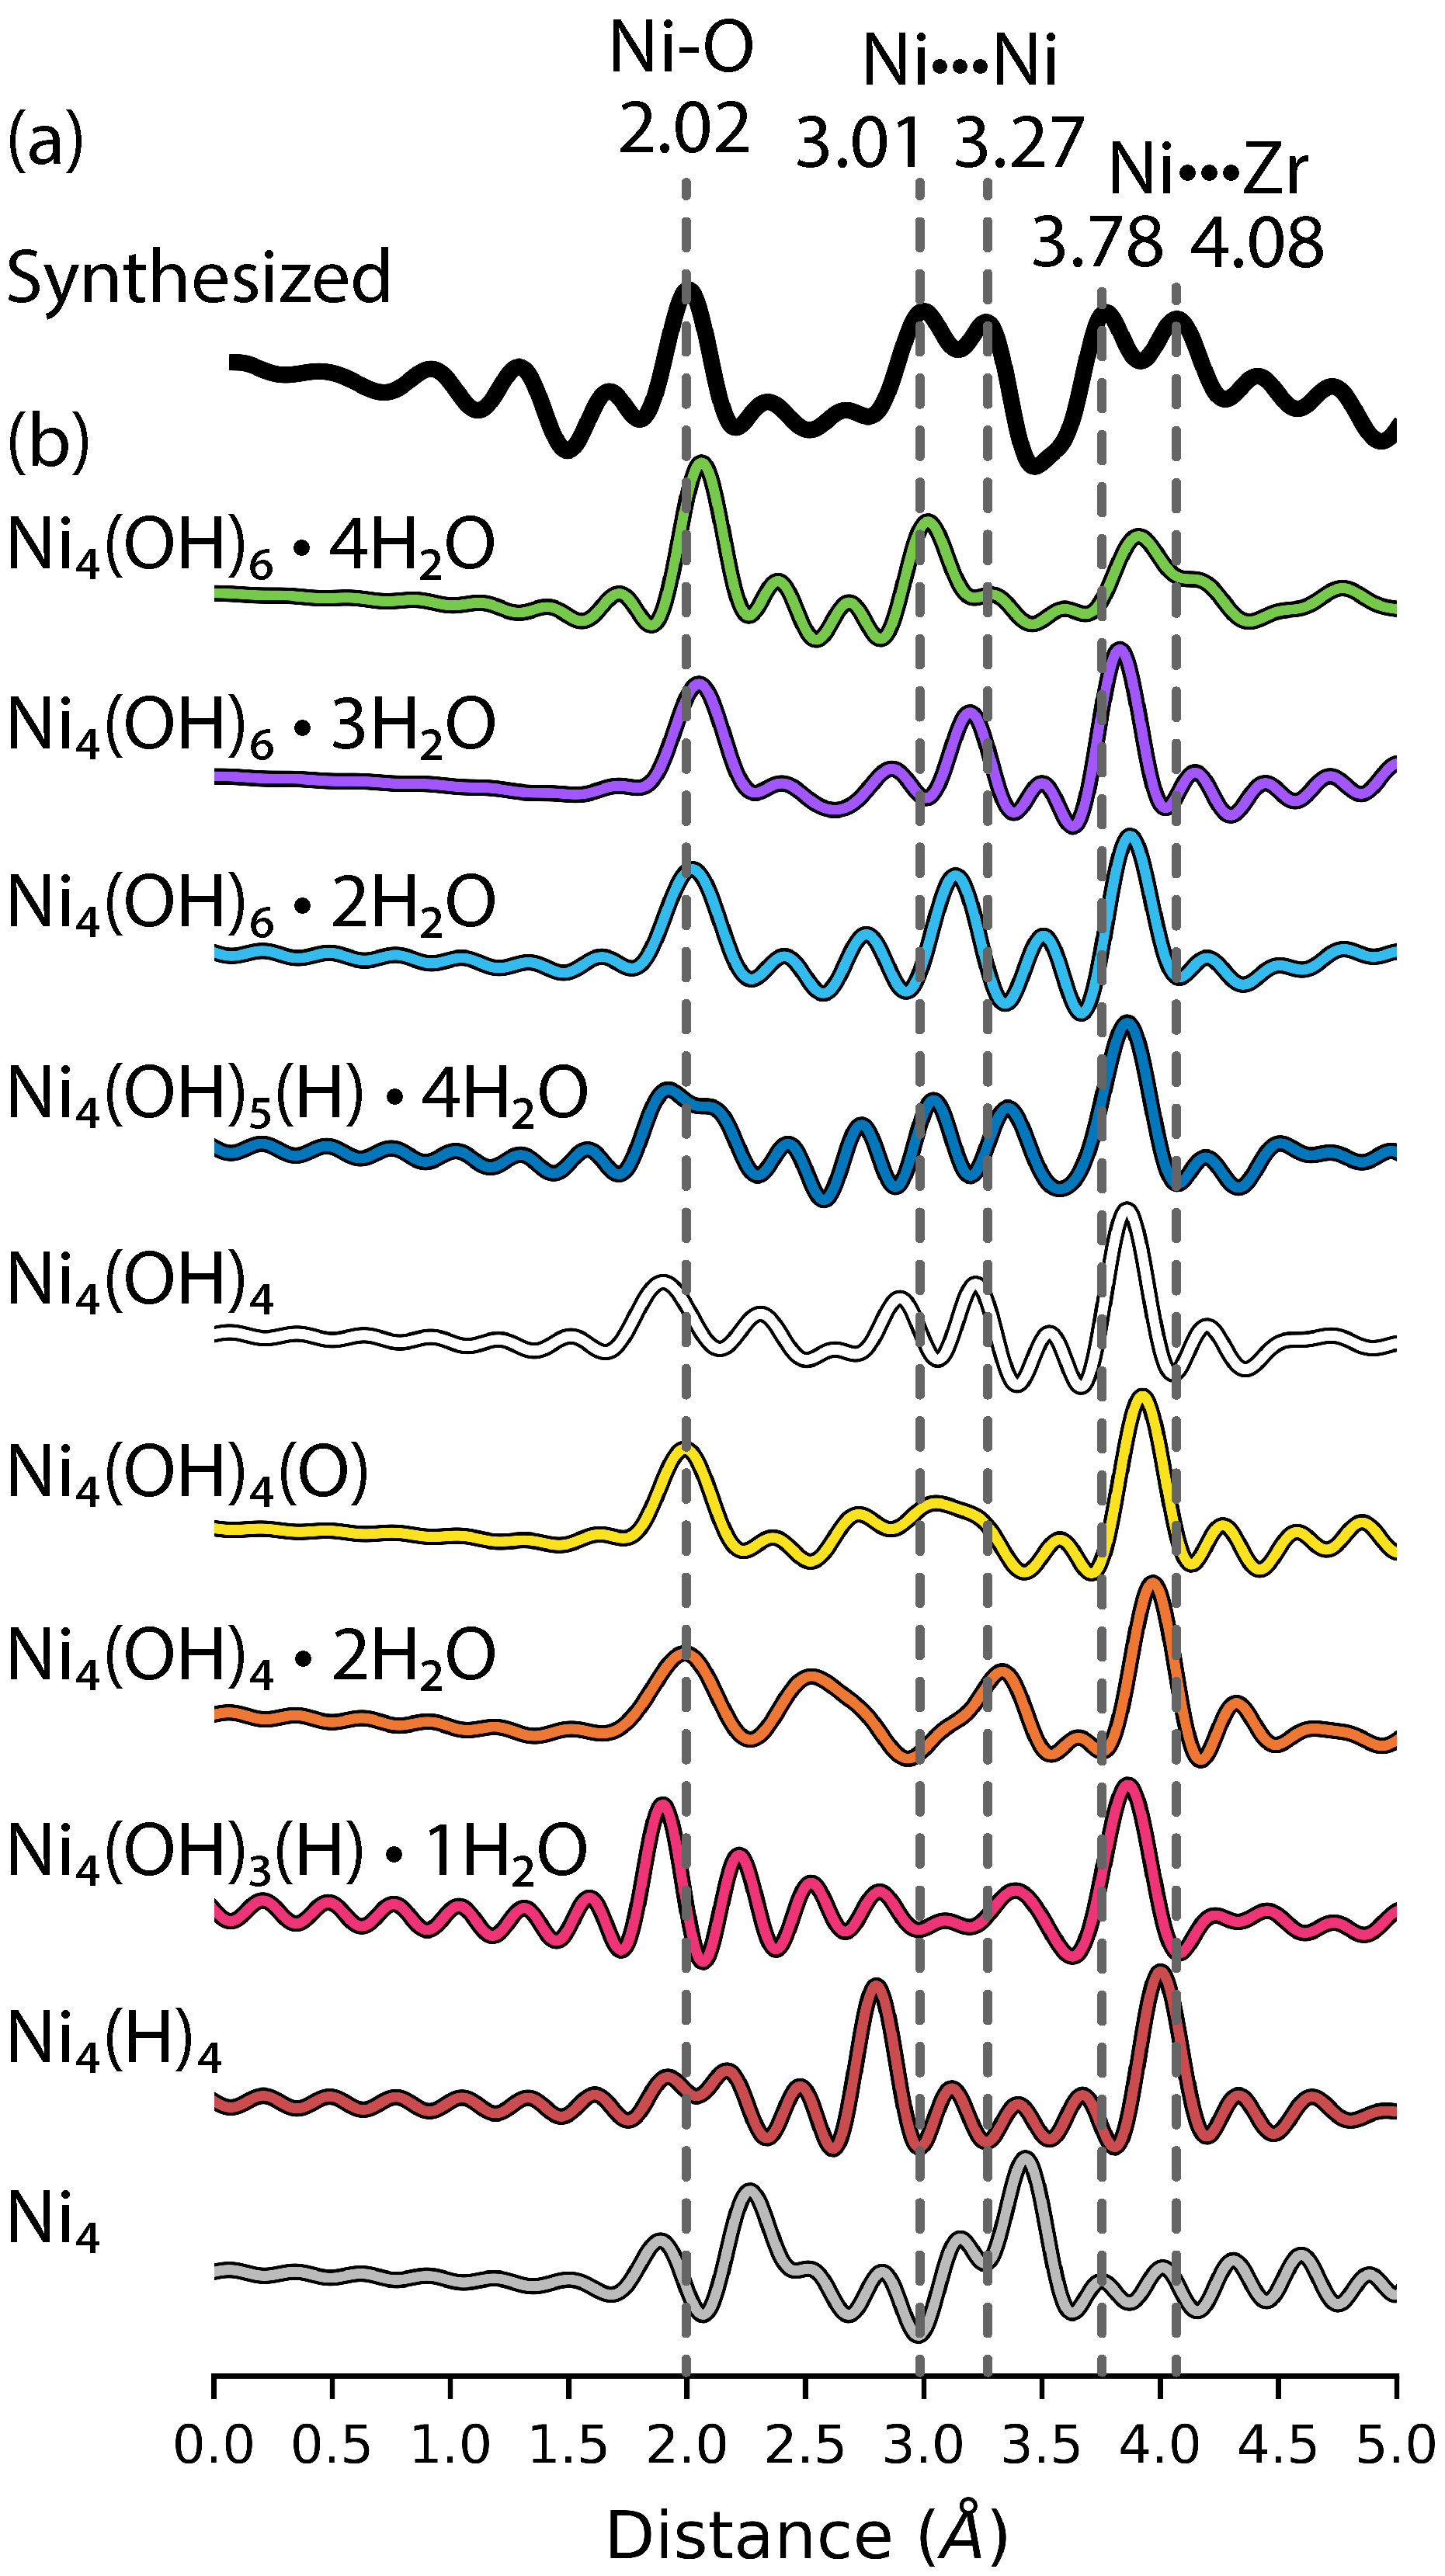
\includegraphics[width=0.60\textwidth]{zi-images/04-SI-images/2022-single-full_dPDF.png}
    \caption{d-PDFs for (a) the synthesized structure and (b) all simulated structures representing thermodynamic minima. The following naming convention is used: \ce{Ni4(OH)6.4H2O} (green), \ce{Ni4(OH)6.3H2O} (purple), \ce{Ni4(OH)6.2H2O} (cyan), \ce{Ni4(OH)5(H).4H2O} (blue), \ce{Ni4(OH)4} (white), \ce{Ni4(OH)4(O)} (yellow), \ce{Ni4(OH)4.2H2O} (orange), \ce{Ni4(OH)3(H).H2O} (magenta), \ce{Ni4(H)4} (red), and \ce{Ni4} (gray). Gray dotted lines indicate key distances observed for the synthesized structure, which are also annotated on the figure.
    }
    \label{fig:SI-all-dPDFs}
\end{figure}


%%%%%%%%%%%%%%%%%%%%%%%%%%%%%%%%%%%%%%%%%%%%%%%%%%%%%%%%%%%%%%%%%%%%%
%% Variable Ni Content Phase Diagram
%%%%%%%%%%%%%%%%%%%%%%%%%%%%%%%%%%%%%%%%%%%%%%%%%%%%%%%%%%%%%%%%%%%%%
\newpage
\section{Variable \ce{Ni} Content Phase Diagram}
\begin{figure}[H]
    \centering
    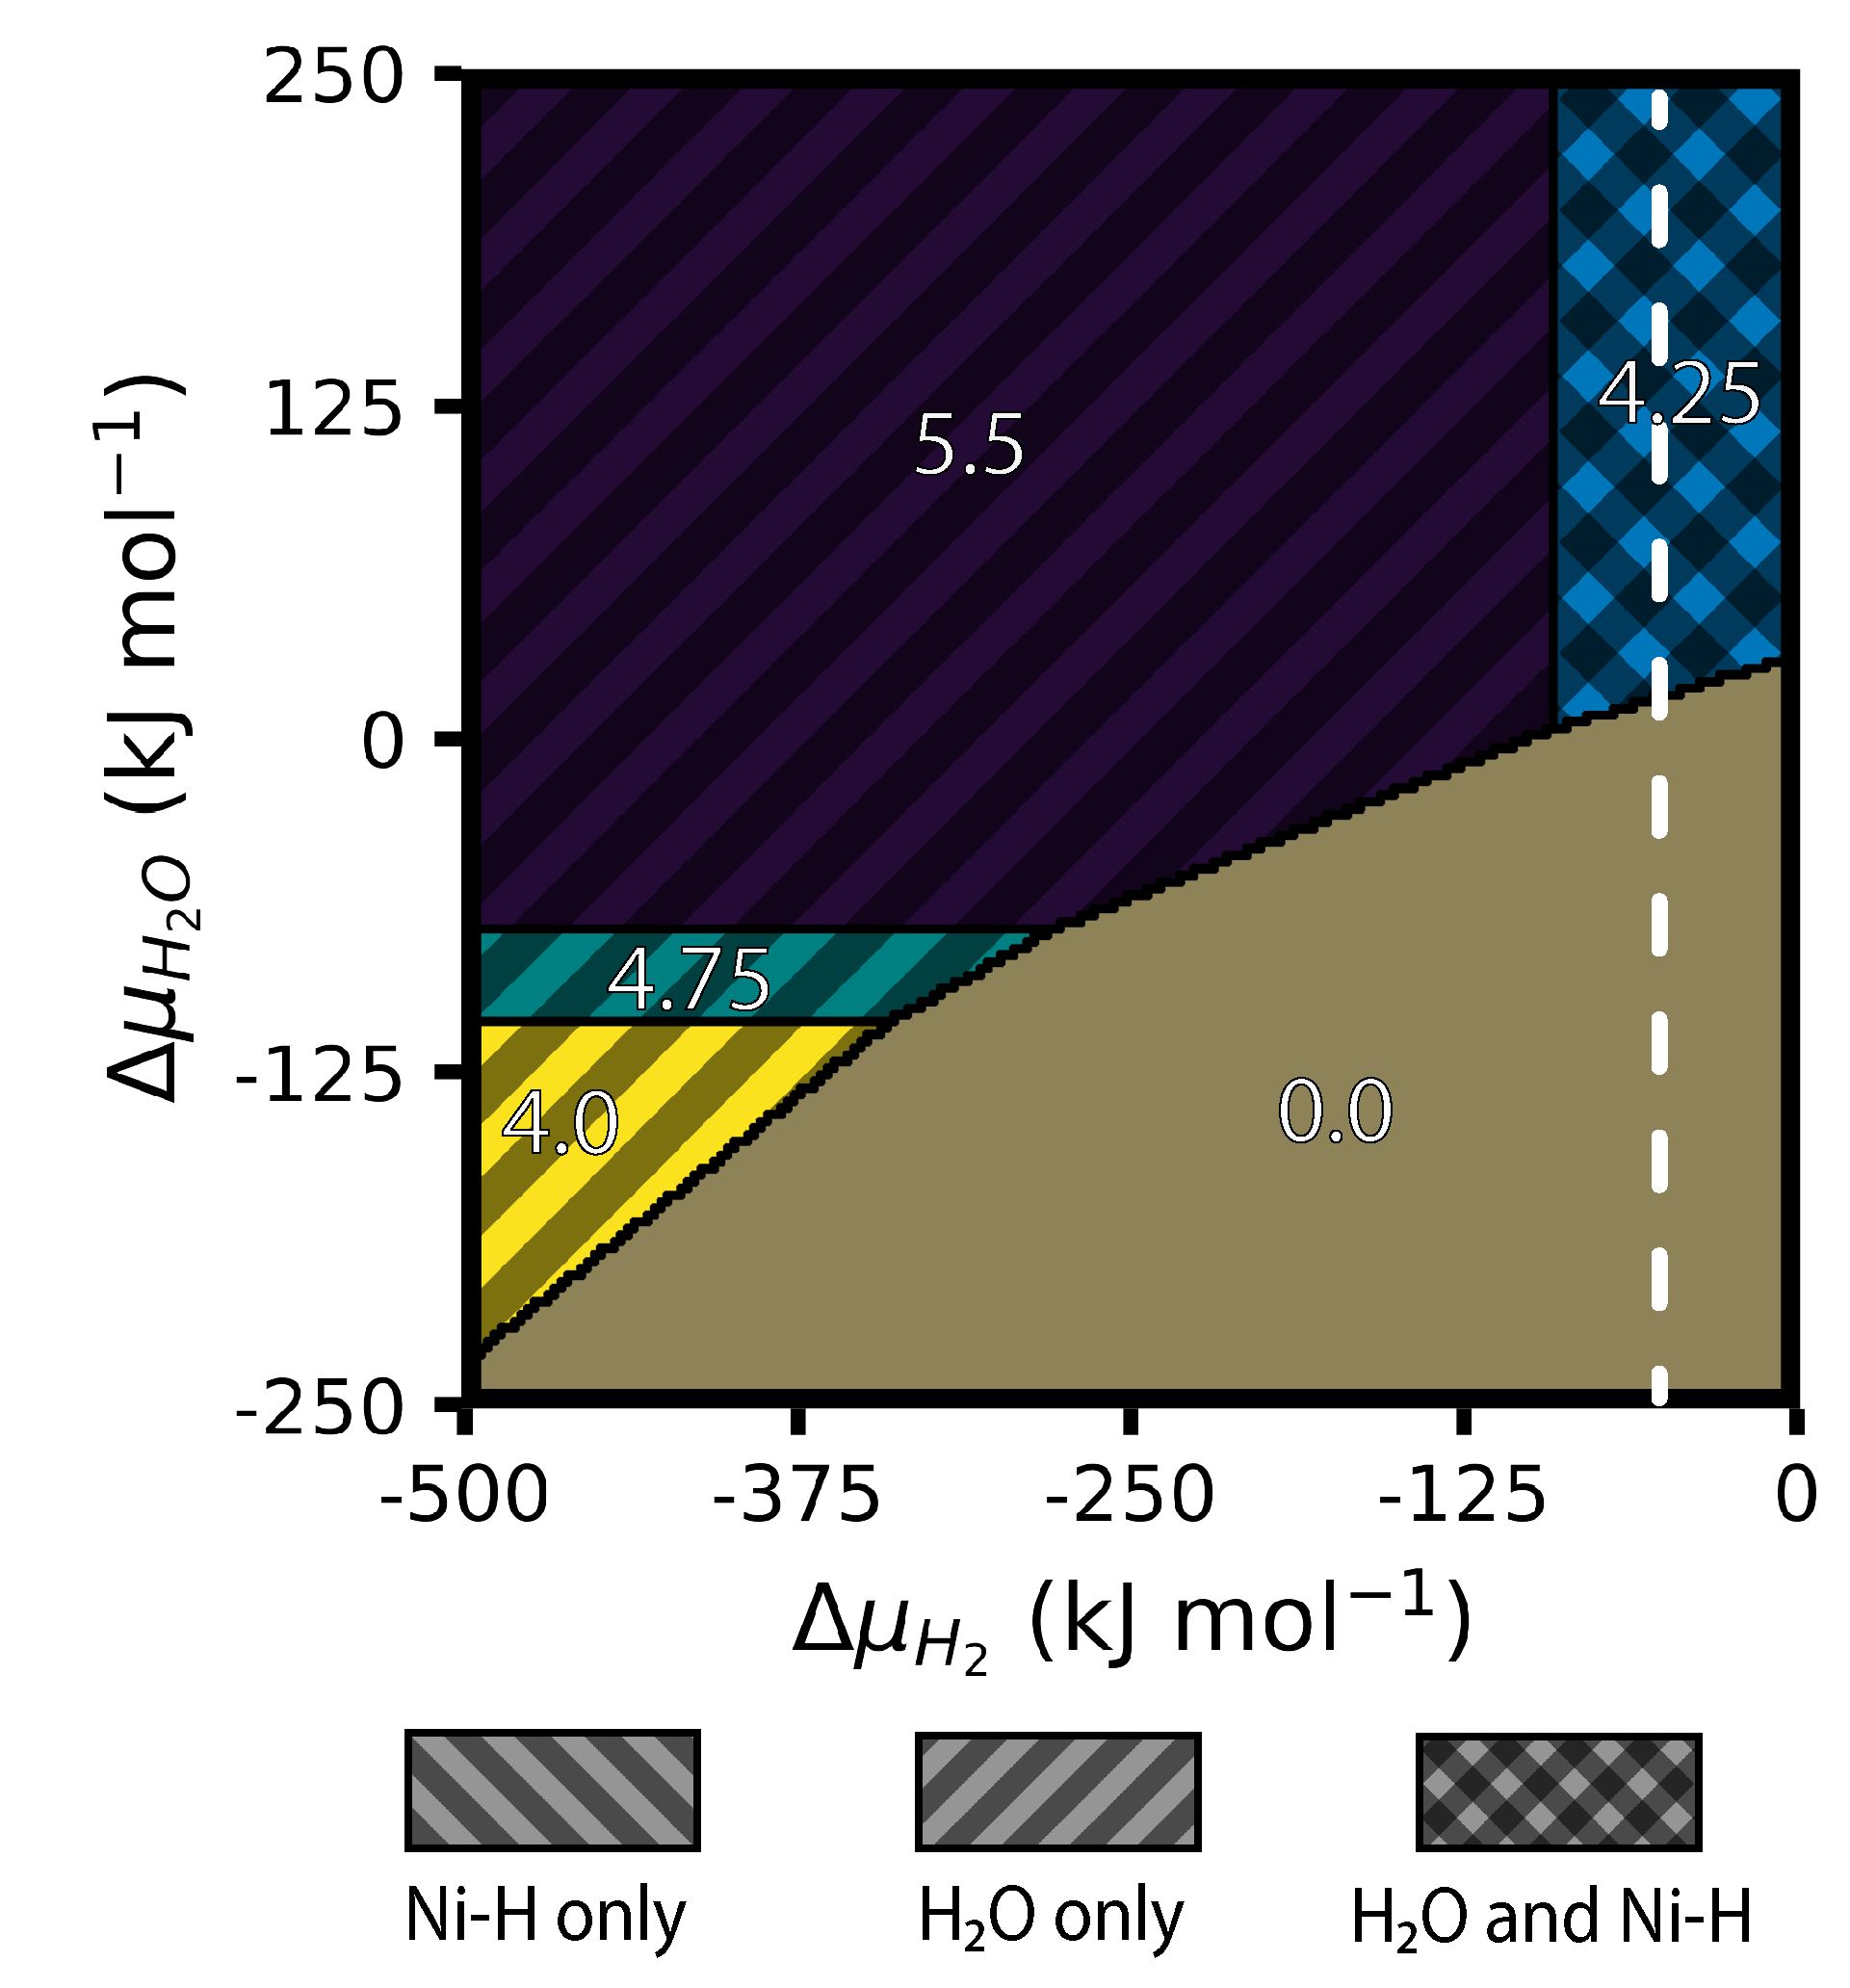
\includegraphics[width=0.60\textwidth]{zi-images/04-SI-images/2021-SI-phase-diagram-trans_Ni.png}
    \caption{
        Calculated phase diagram for the \ce{Ni4} cluster presented as a function of $\Delta \mu_{\ce{H2}}$, $\Delta \mu_{\ce{H2O}}$, and $\Delta \mu_{\ce{Ni}}$. The $\Delta \mu_{\ce{Ni}}$, referenced from a bulk \ce{Ni}, allows for variable \ce{Ni} composition. The different colored regions indicate different structures. The \ce{Ni-O} coordination numbers are presented on the diagram. The vibrational contributions to the free energy are not considered here. 
    }
    \label{fig:SI-variable-Ni-content}
\end{figure}

Figure~\ref{fig:SI-variable-Ni-content} considered the thermodynamic landscape of \ce{Ni} clusters with variable \ce{Ni} composition. Only structures \ce{Ni4(OH)4(O)} (yellow) and \ce{Ni4(OH)5(H).4H2O} (blue) appear on the phase diagram presented in the main text (Figure~4). Structure \ce{Ni4(OH)6.1H2O} (teal), which does not appear on Figure~4 but is discussed in the main text because of the d-PDF, now appears on the phase diagram given that vibrational contributions are considered. The remaining two structures, NU-1000 (gold) and \ce{Ni4(OH)6.4H2O} (violet), represent the bare MOF with a \ce{Ni}-nanoparticle (gold) and another structure with four coordinating \ce{H2O} ligands and six interconnecting \ce{OH}-ligands, respectively. For \ce{Cu}-oxo clusters supported on NU-1000, the nanoparticle formation is common under reducing conditions.\cite{Yang2020} Similar to the prior discussion about \ce{Ni4(OH)6.1H2O} (teal), \ce{Ni4(OH)6.4H2O} (violet) compared with the structure appearing in the main text (\ce{Ni4(OH)6.4H2O} (green)), but does not appear on the Figure~4 when vibrational contributions are considered. 

%%%%%%%%%%%%%%%%%%%%%%%%%%%%%%%%%%%%%%%%%%%%%%%%%%%%%%%%%%%%%%%%%%%%%
%% Expanded Conditions
%%%%%%%%%%%%%%%%%%%%%%%%%%%%%%%%%%%%%%%%%%%%%%%%%%%%%%%%%%%%%%%%%%%%%
\newpage
\section{Phase Diagram Expanded Conditions}
\begin{figure}[H]
    \centering
    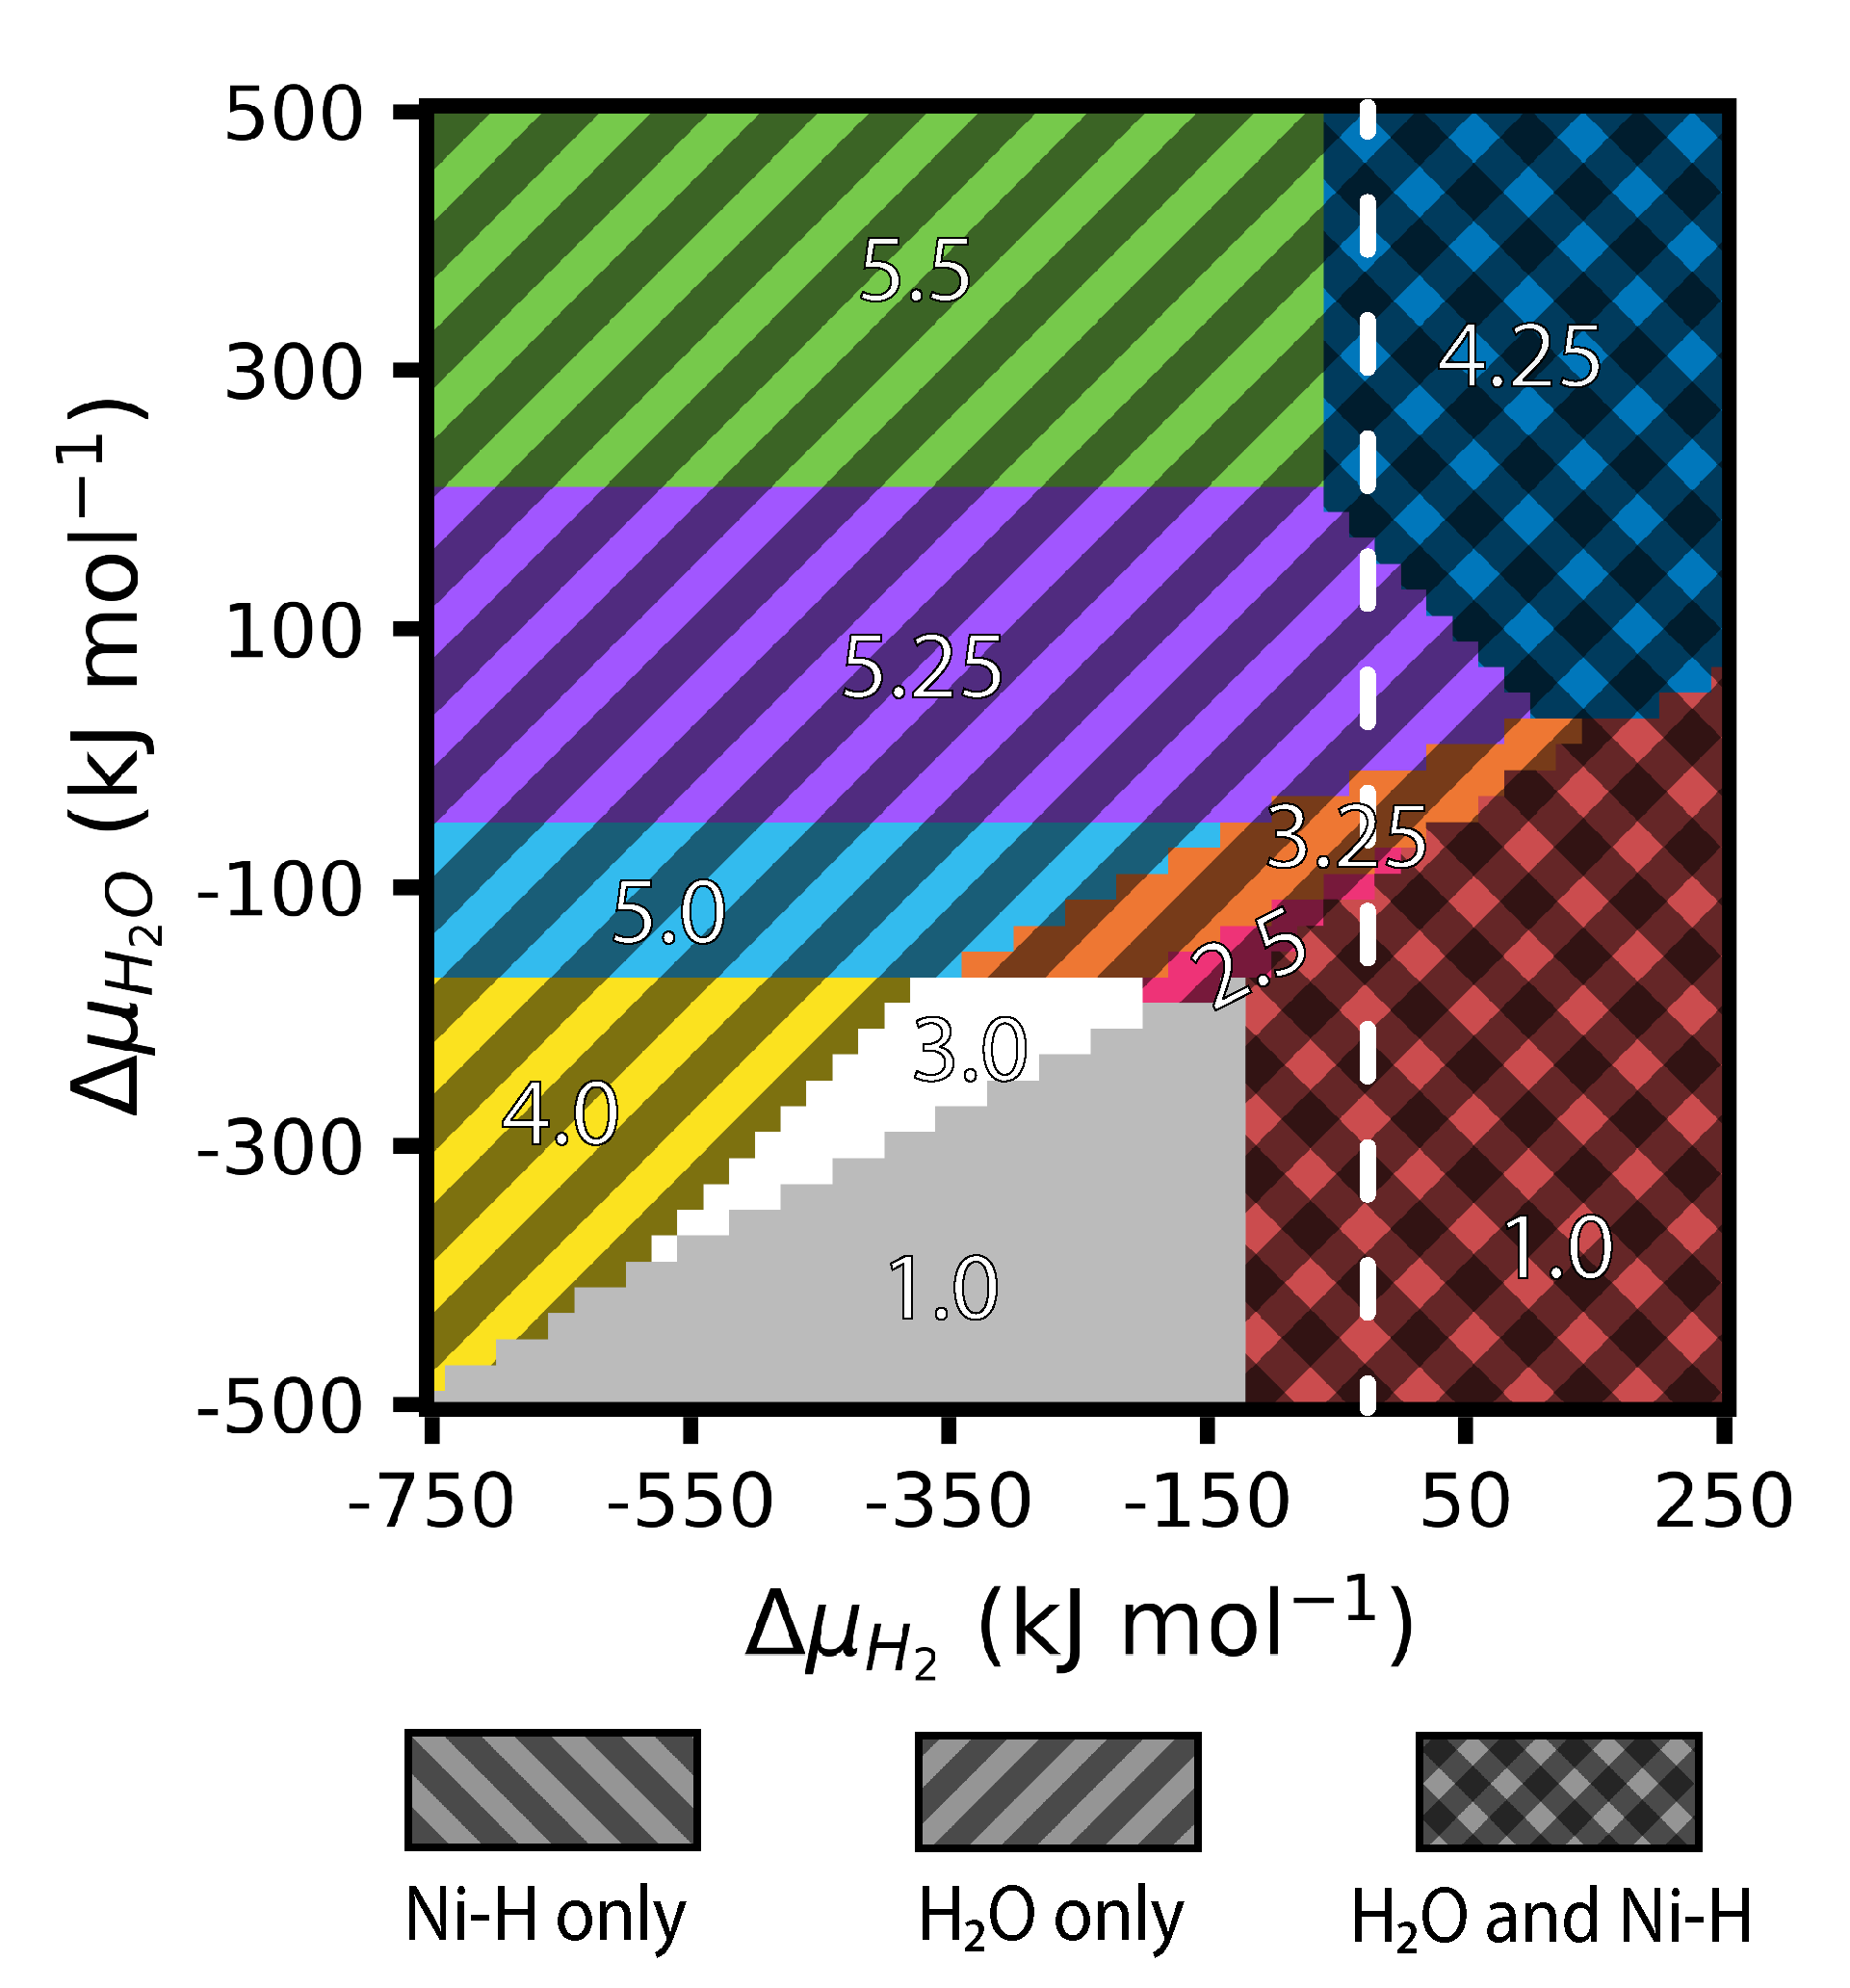
\includegraphics[width=0.60\textwidth]{zi-images/04-SI-images/2021-SI-phase-diagram-expanded.png}
    \caption{
        Calculated phase diagram for the \ce{Ni4} cluster presented as a function $\Delta \mu_{\ce{H2}}$ and $\Delta \mu_{\ce{H2O}}$. The conditions for $\Delta \mu_{\ce{H2}}$ and $\Delta \mu_{\ce{H2O}}$ are expanded from the conditions presented in Figure~4 (main text) to show that the structures considered in the main text are the only structures present on the phase diagram. The different colored regions indicate different structures, following the same key as in Figure~\ref{fig:SI-all-dPDFs}. 
    }
    \label{fig:SI-expanded-conditions}
\end{figure}

%%%%%%%%%%%%%%%%%%%%%%%%%%%%%%%%%%%%%%%%%%%%%%%%%%%%%%%%%%%%%%%%%%%%%
%% Phase Diagram Structures
%%%%%%%%%%%%%%%%%%%%%%%%%%%%%%%%%%%%%%%%%%%%%%%%%%%%%%%%%%%%%%%%%%%%%
\newpage
\section{Phase Diagram Structures}
All thermodynamic minima structures according to \textit{ab initio} thermodynamic analysis are presented in Figures~S\ref{fig:SI-dPDF-green} to~S\ref{fig:SI-dPDF-red}. Each figure includes the (a) d-PDF, (b) the schematic drawing, and (c) the atomic rendering for that structure. 

\begin{figure}[H]
    \centering
    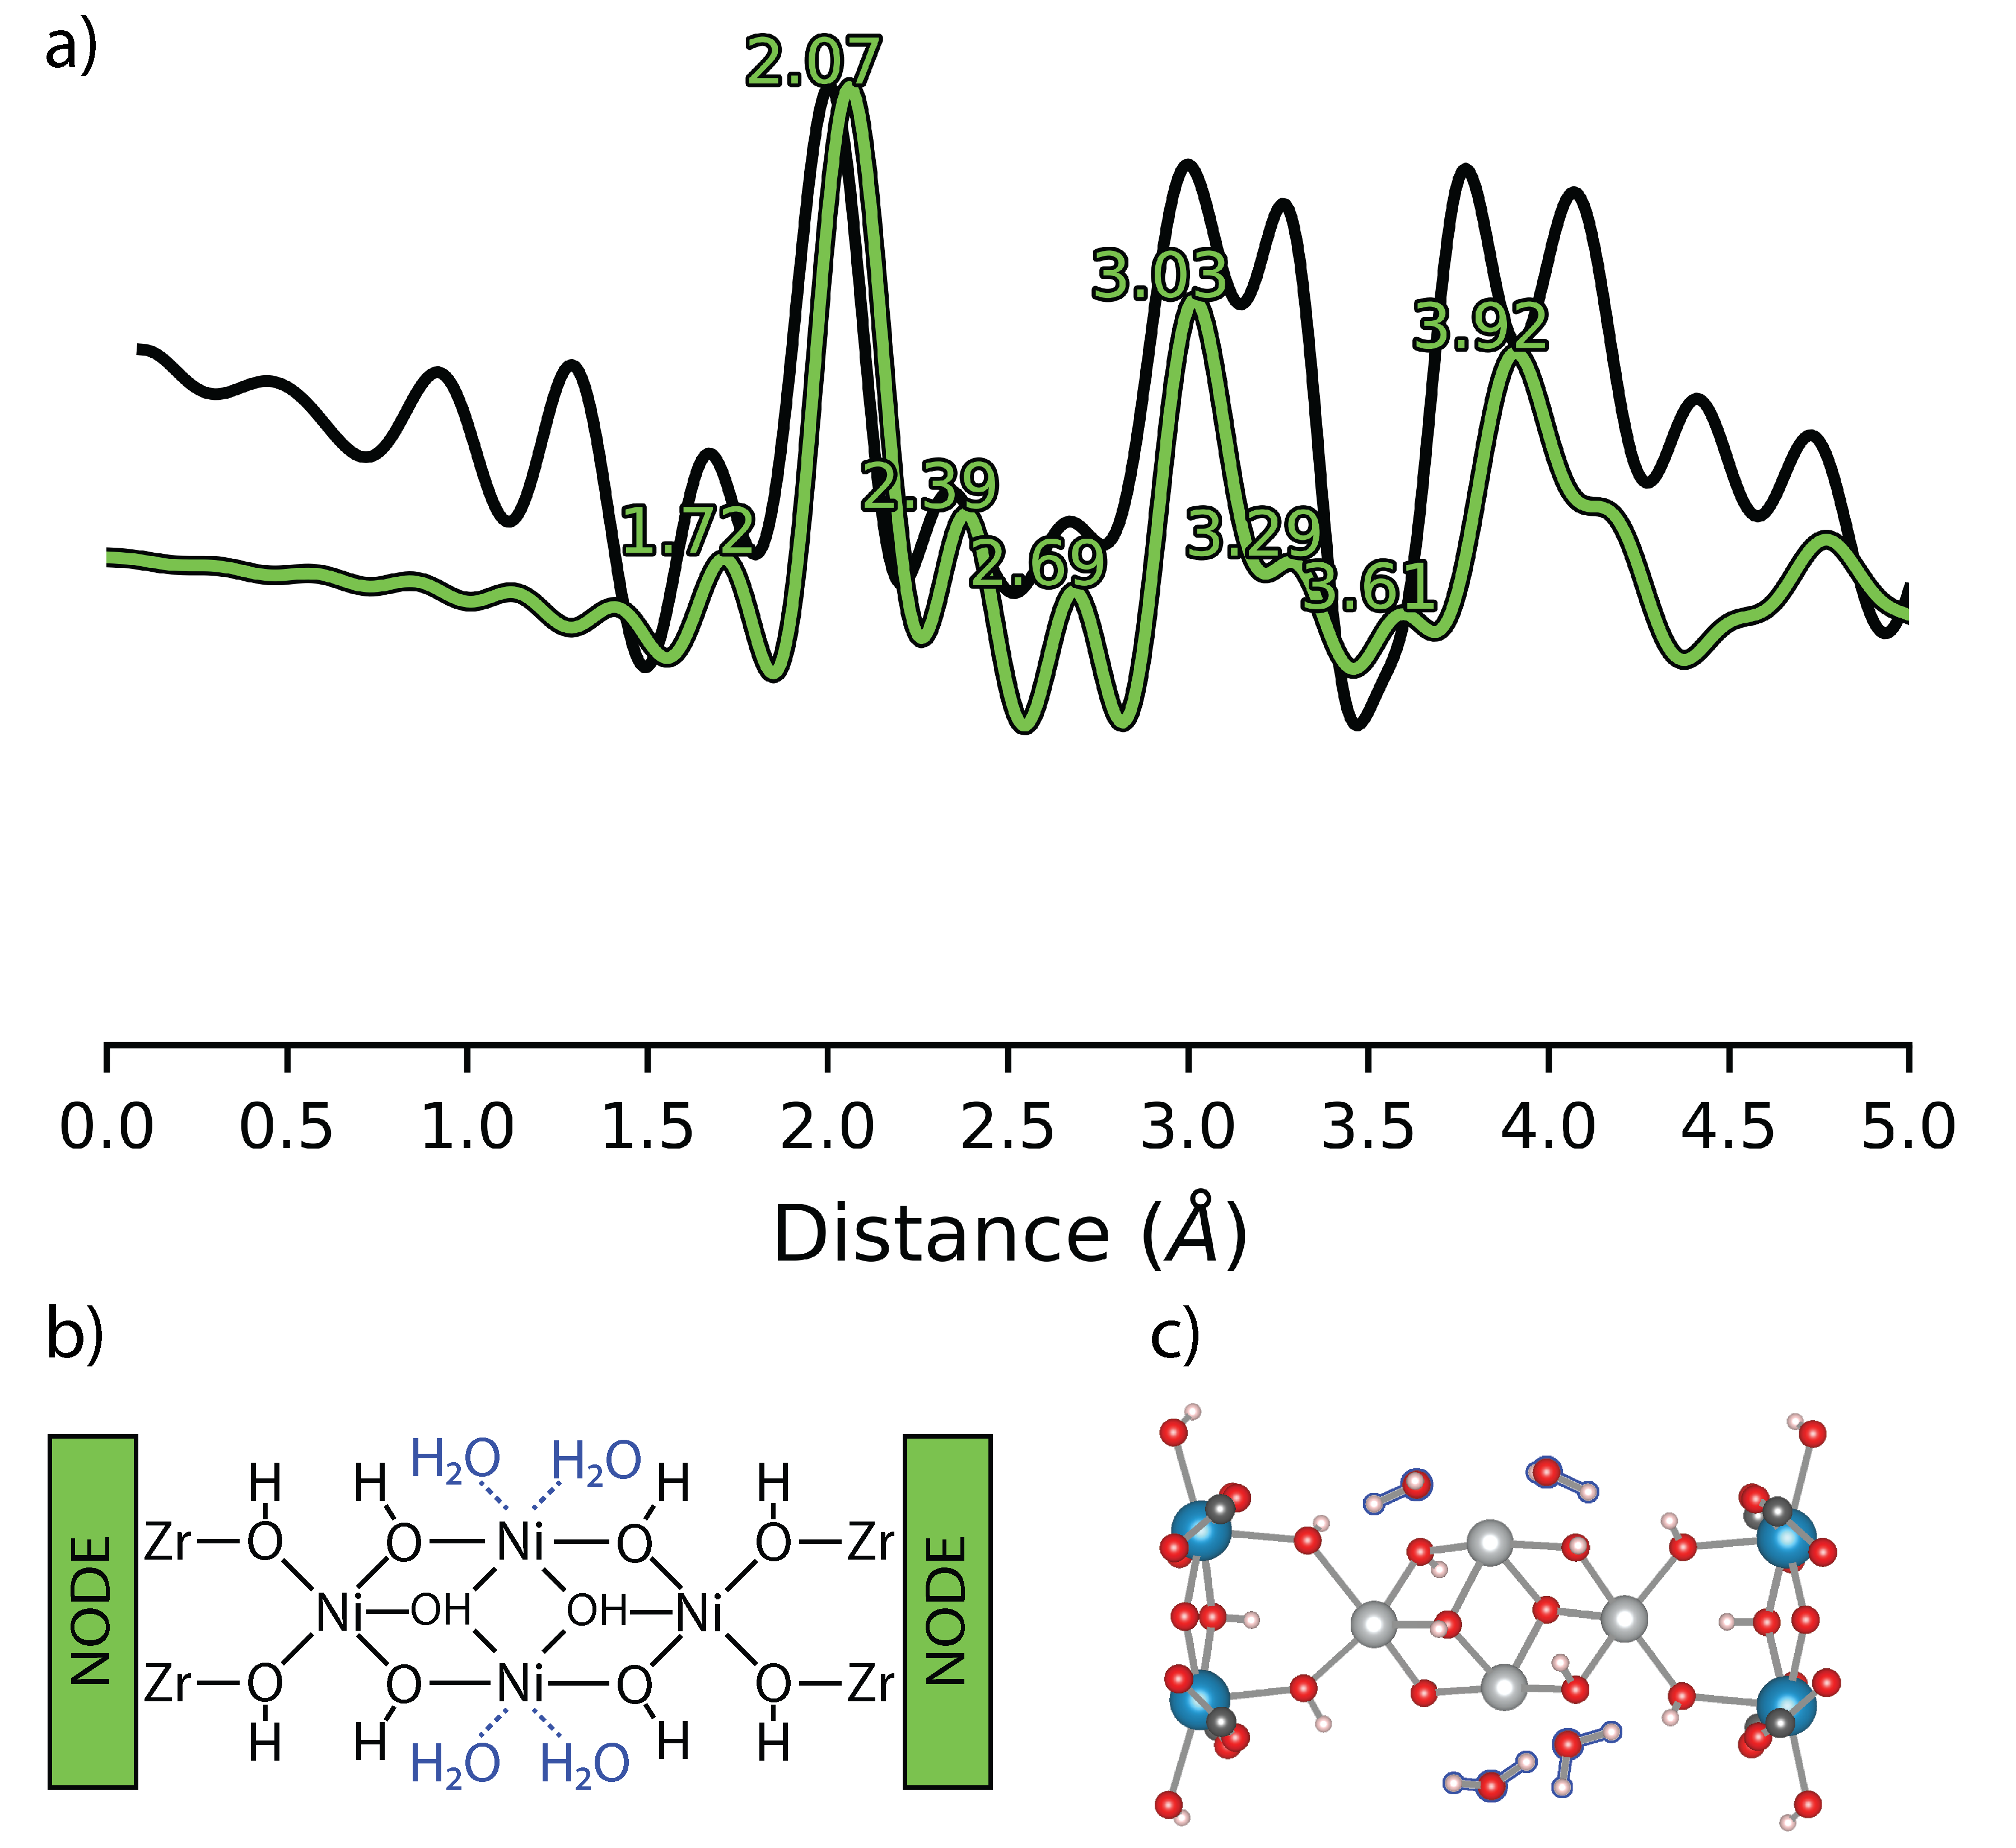
\includegraphics[width=0.75\textwidth]{zi-images/04-SI-images/SI-dPDF-Green.png}
    \caption{The local structural information for the \ce{Ni4(OH)6.4H2O} (green) structure, presented as the (a) d-PDF, (b) the schematic representation, and (c) a 3D rendering. The key distances for \ce{Ni4(OH)6.4H2O} (green) based on d-PDF analysis include a \ce{Ni-O} peak at 2.02 {\AA}, a \ce{Ni{\Compactcdots}Ni} peak at 3.03 {\AA}, and a \ce{Ni{\Compactcdots}Zr} peak at 3.92 {\AA}, as seen in (a). The structure does not exhibit any \ce{Ni{\Compactcdots}Ni} or \ce{Ni{\Compactcdots}Zr} peak splitting.
    }
    \label{fig:SI-dPDF-green}
\end{figure}
    
\begin{figure}[H]
    \centering
    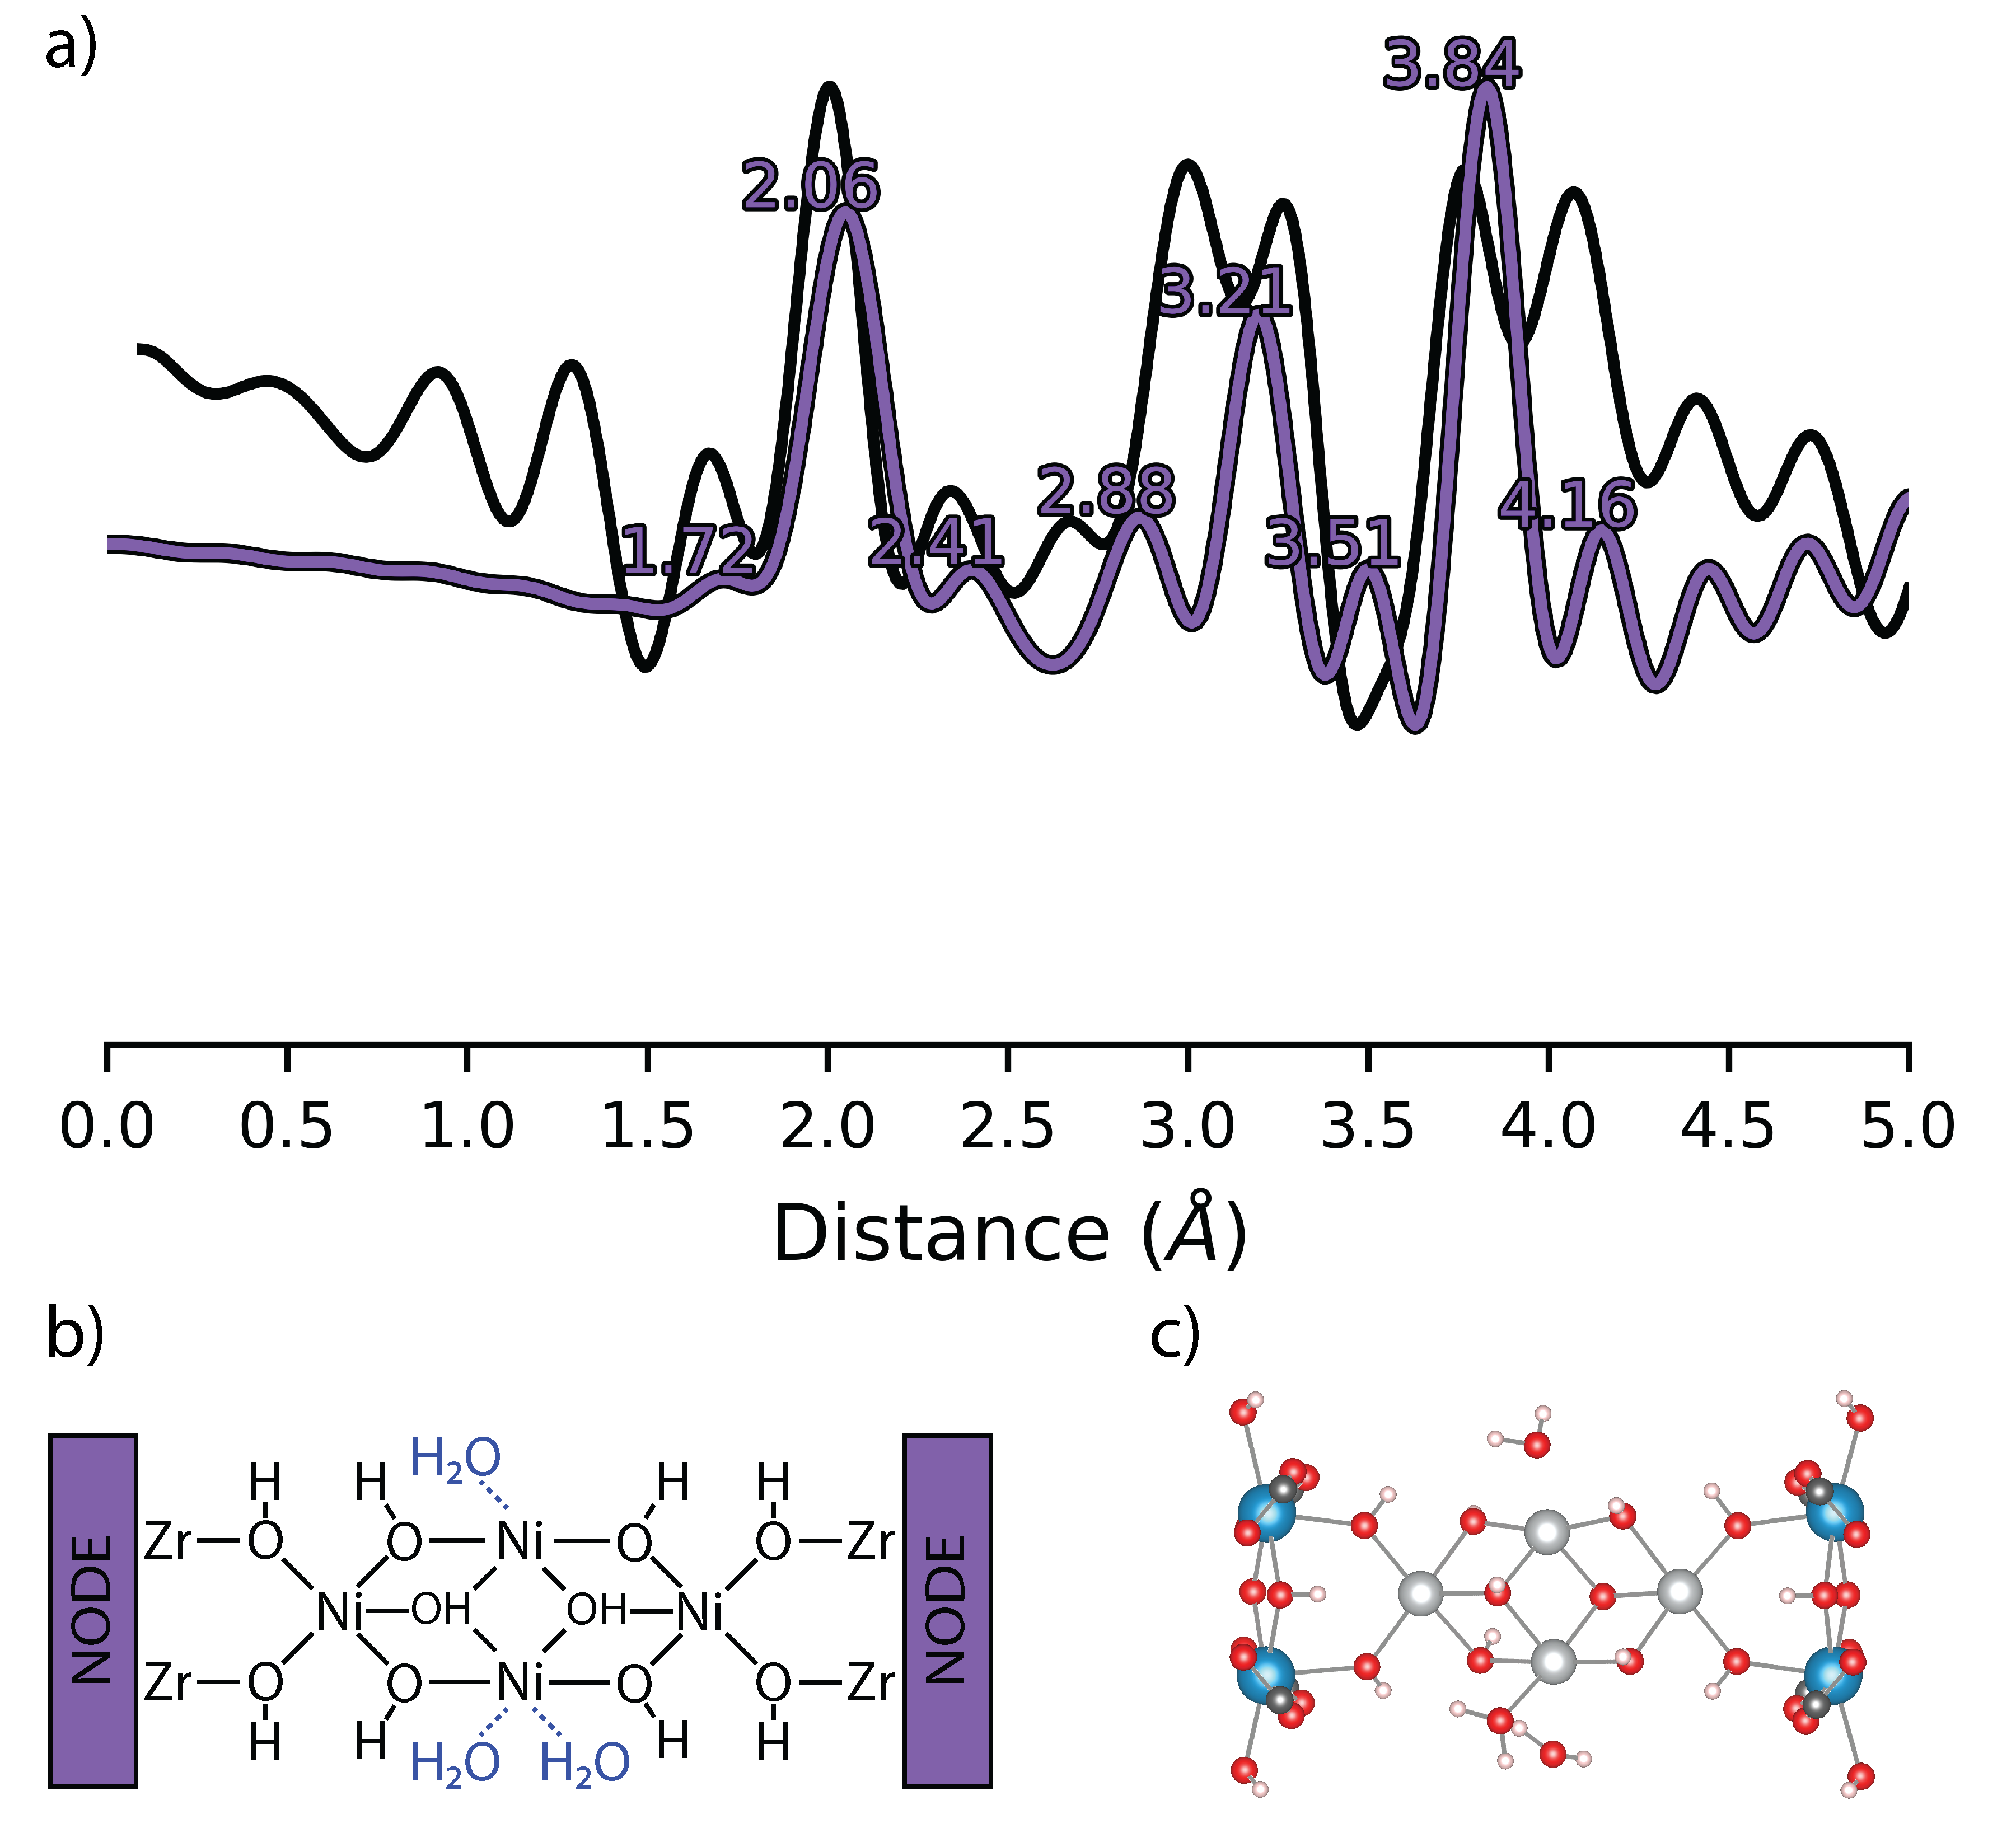
\includegraphics[width=0.75\textwidth]{zi-images/04-SI-images/SI-dPDF-Purple.png}
    \caption{The local structural information for the \ce{Ni4(OH)6.3H2O} (purple) structure, presented as the (a) d-PDF, (b) the schematic representation, and (c) a 3D rendering. The key distances for \ce{Ni4(OH)6.3H2O} (purple) based on d-PDF analysis include a \ce{Ni-O} peak at 2.07 {\AA}, a \ce{Ni{\Compactcdots}Ni} peak at 3.03 {\AA}, and a \ce{Ni{\Compactcdots}Zr} peak at 3.92 {\AA}, as seen in (a). The structure does not exhibit any \ce{Ni{\Compactcdots}Ni} or \ce{Ni{\Compactcdots}Zr} peak splitting. 
    }
    \label{fig:SI-dPDF-purple}
\end{figure}  
    
\begin{figure}[H]
    \centering
    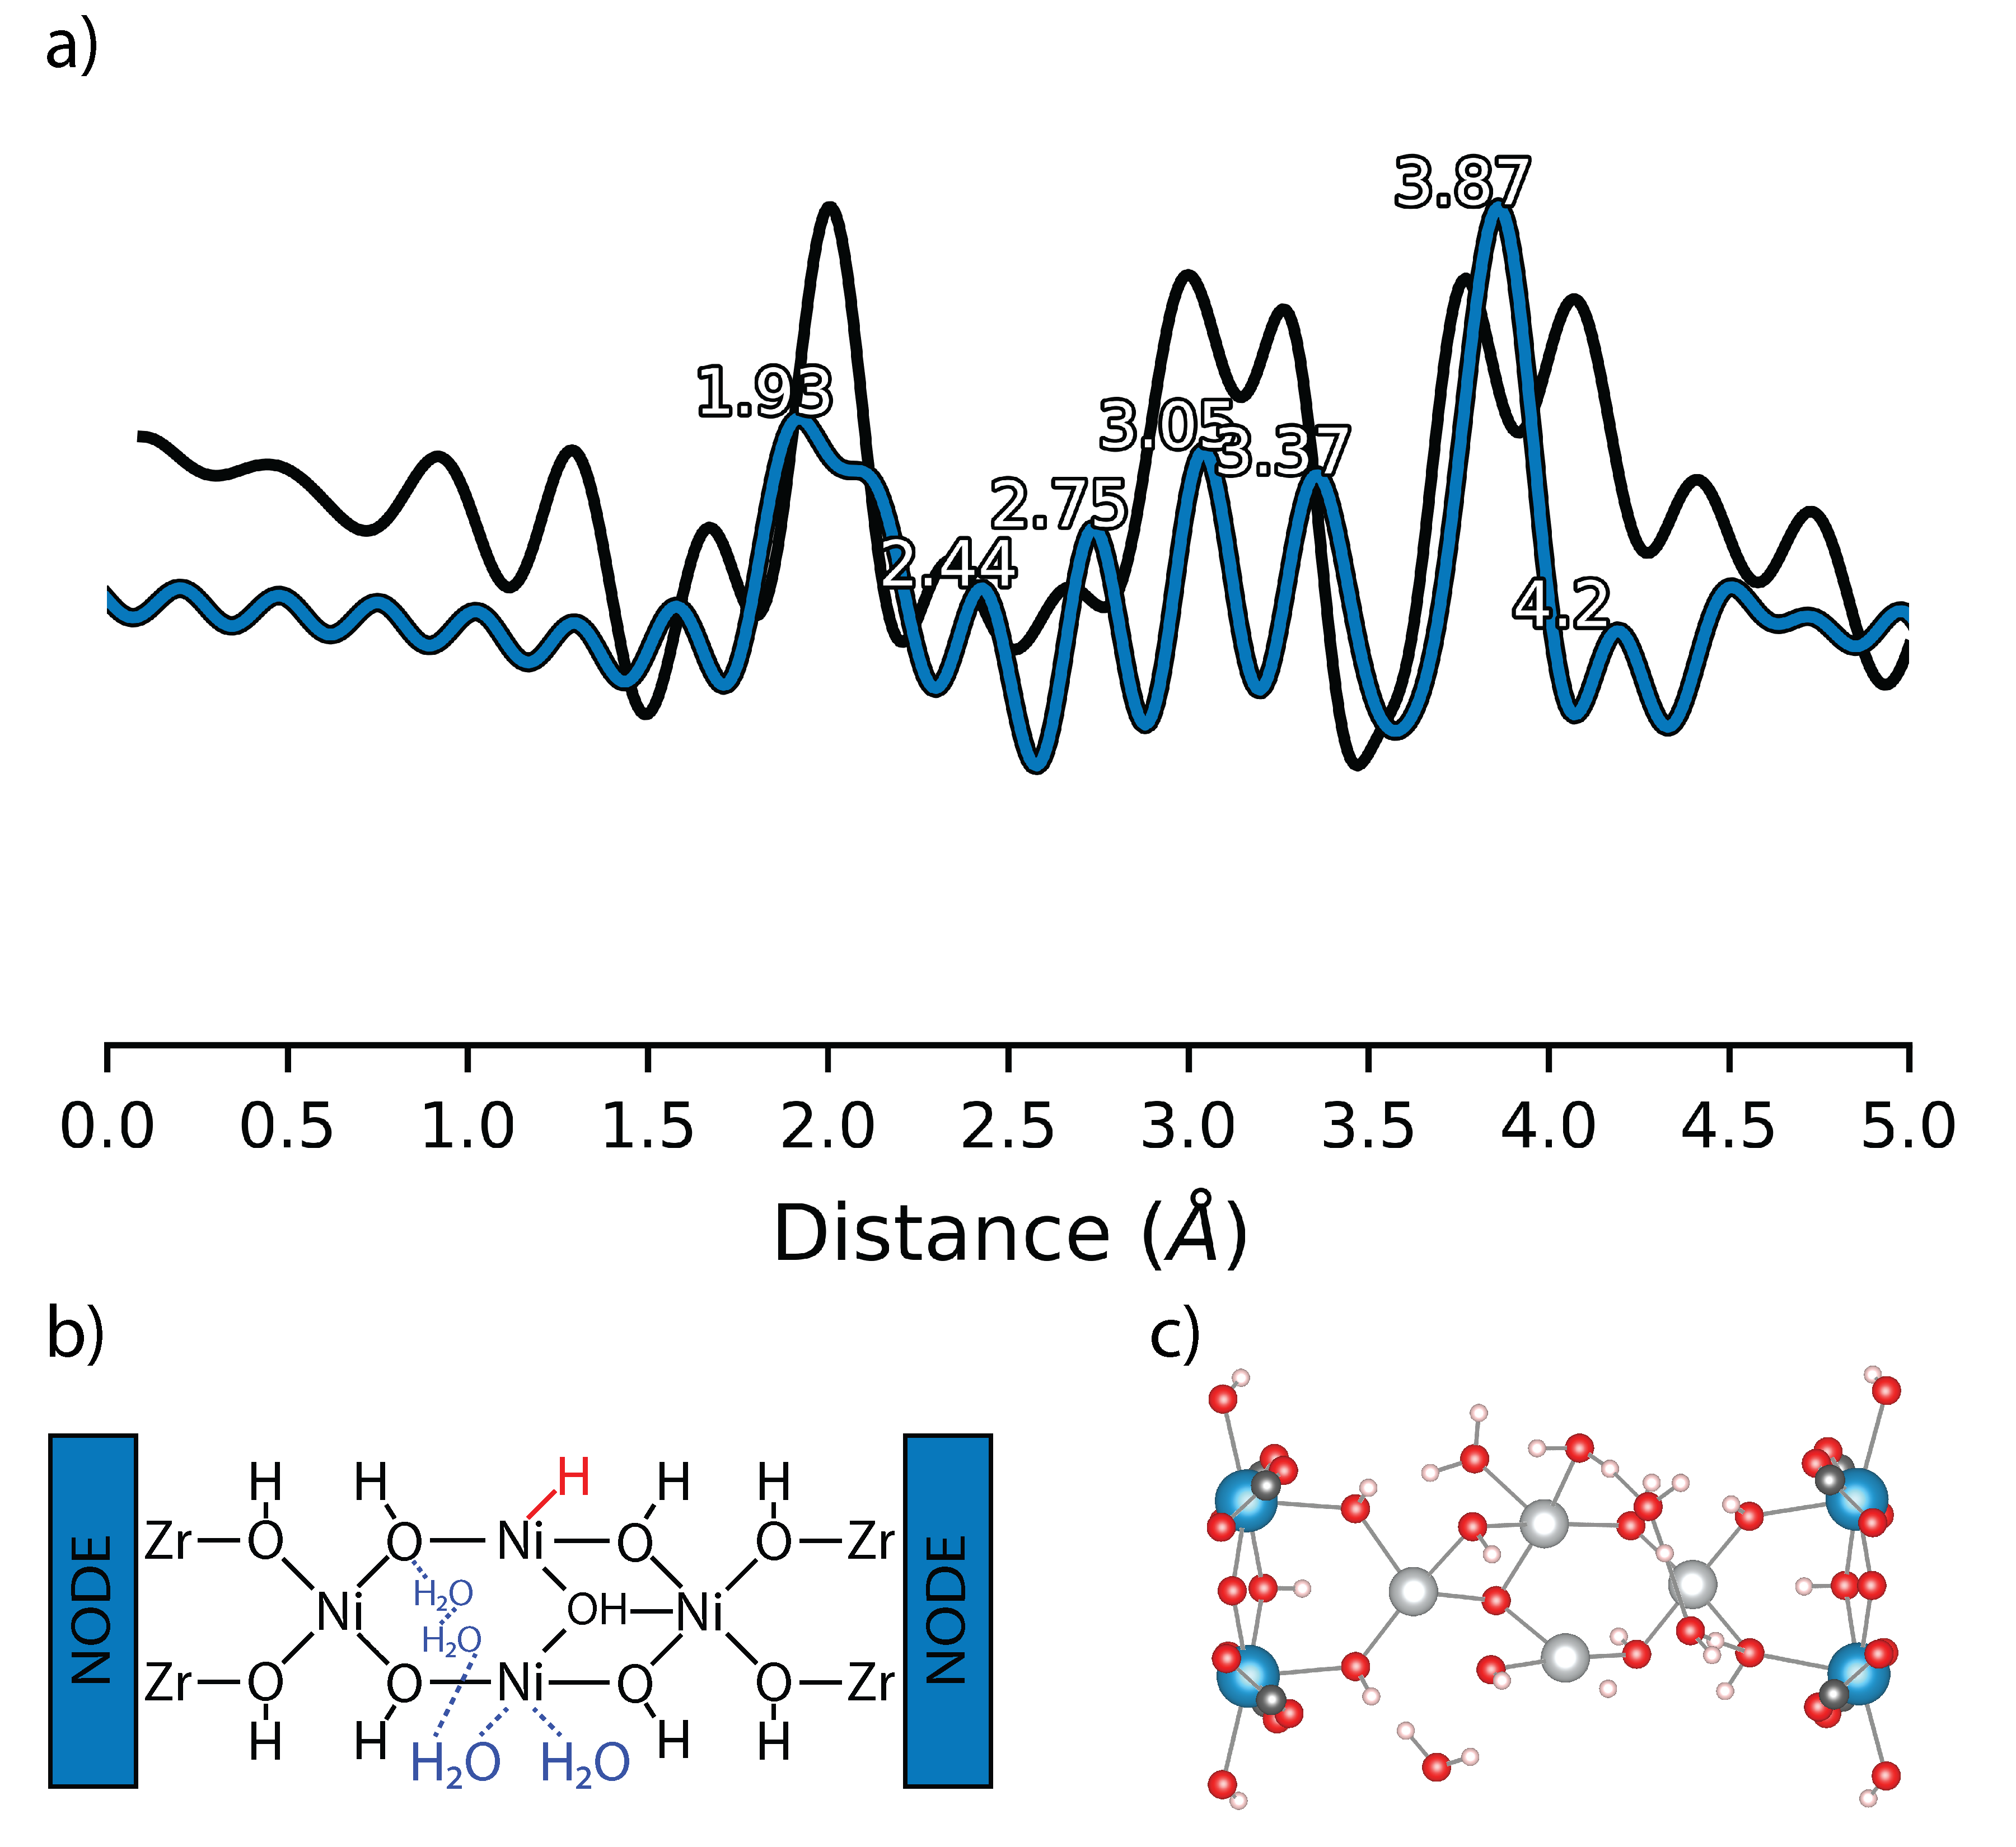
\includegraphics[width=0.75\textwidth]{zi-images/04-SI-images/SI-dPDF-Blue.png}
    \caption{The local structural information for the \ce{Ni4(OH)5(H).4H2O} (blue) structure, presented as the (a) d-PDF, (b) the schematic representation, and (c) a 3D rendering. The key distances for \ce{Ni4(OH)5(H).4H2O} (blue) based on d-PDF analysis include a \ce{Ni-O} peak at 1.93 {\AA}, \ce{Ni{\Compactcdots}Ni} peaks at 2.75, 3.05, and 3.37 {\AA}, and \ce{Ni{\Compactcdots}Zr} peaks at 3.87 {\AA}, as seen in (a). The structure exhibits a triplet of \ce{Ni{\Compactcdots}Ni} peaks and a broadening of the \ce{Ni-O} peak due to the chain of \ce{H2O} molecules. 
    }
    \label{fig:SI-dPDF-blue}
\end{figure}

\begin{figure}[H]
    \centering
    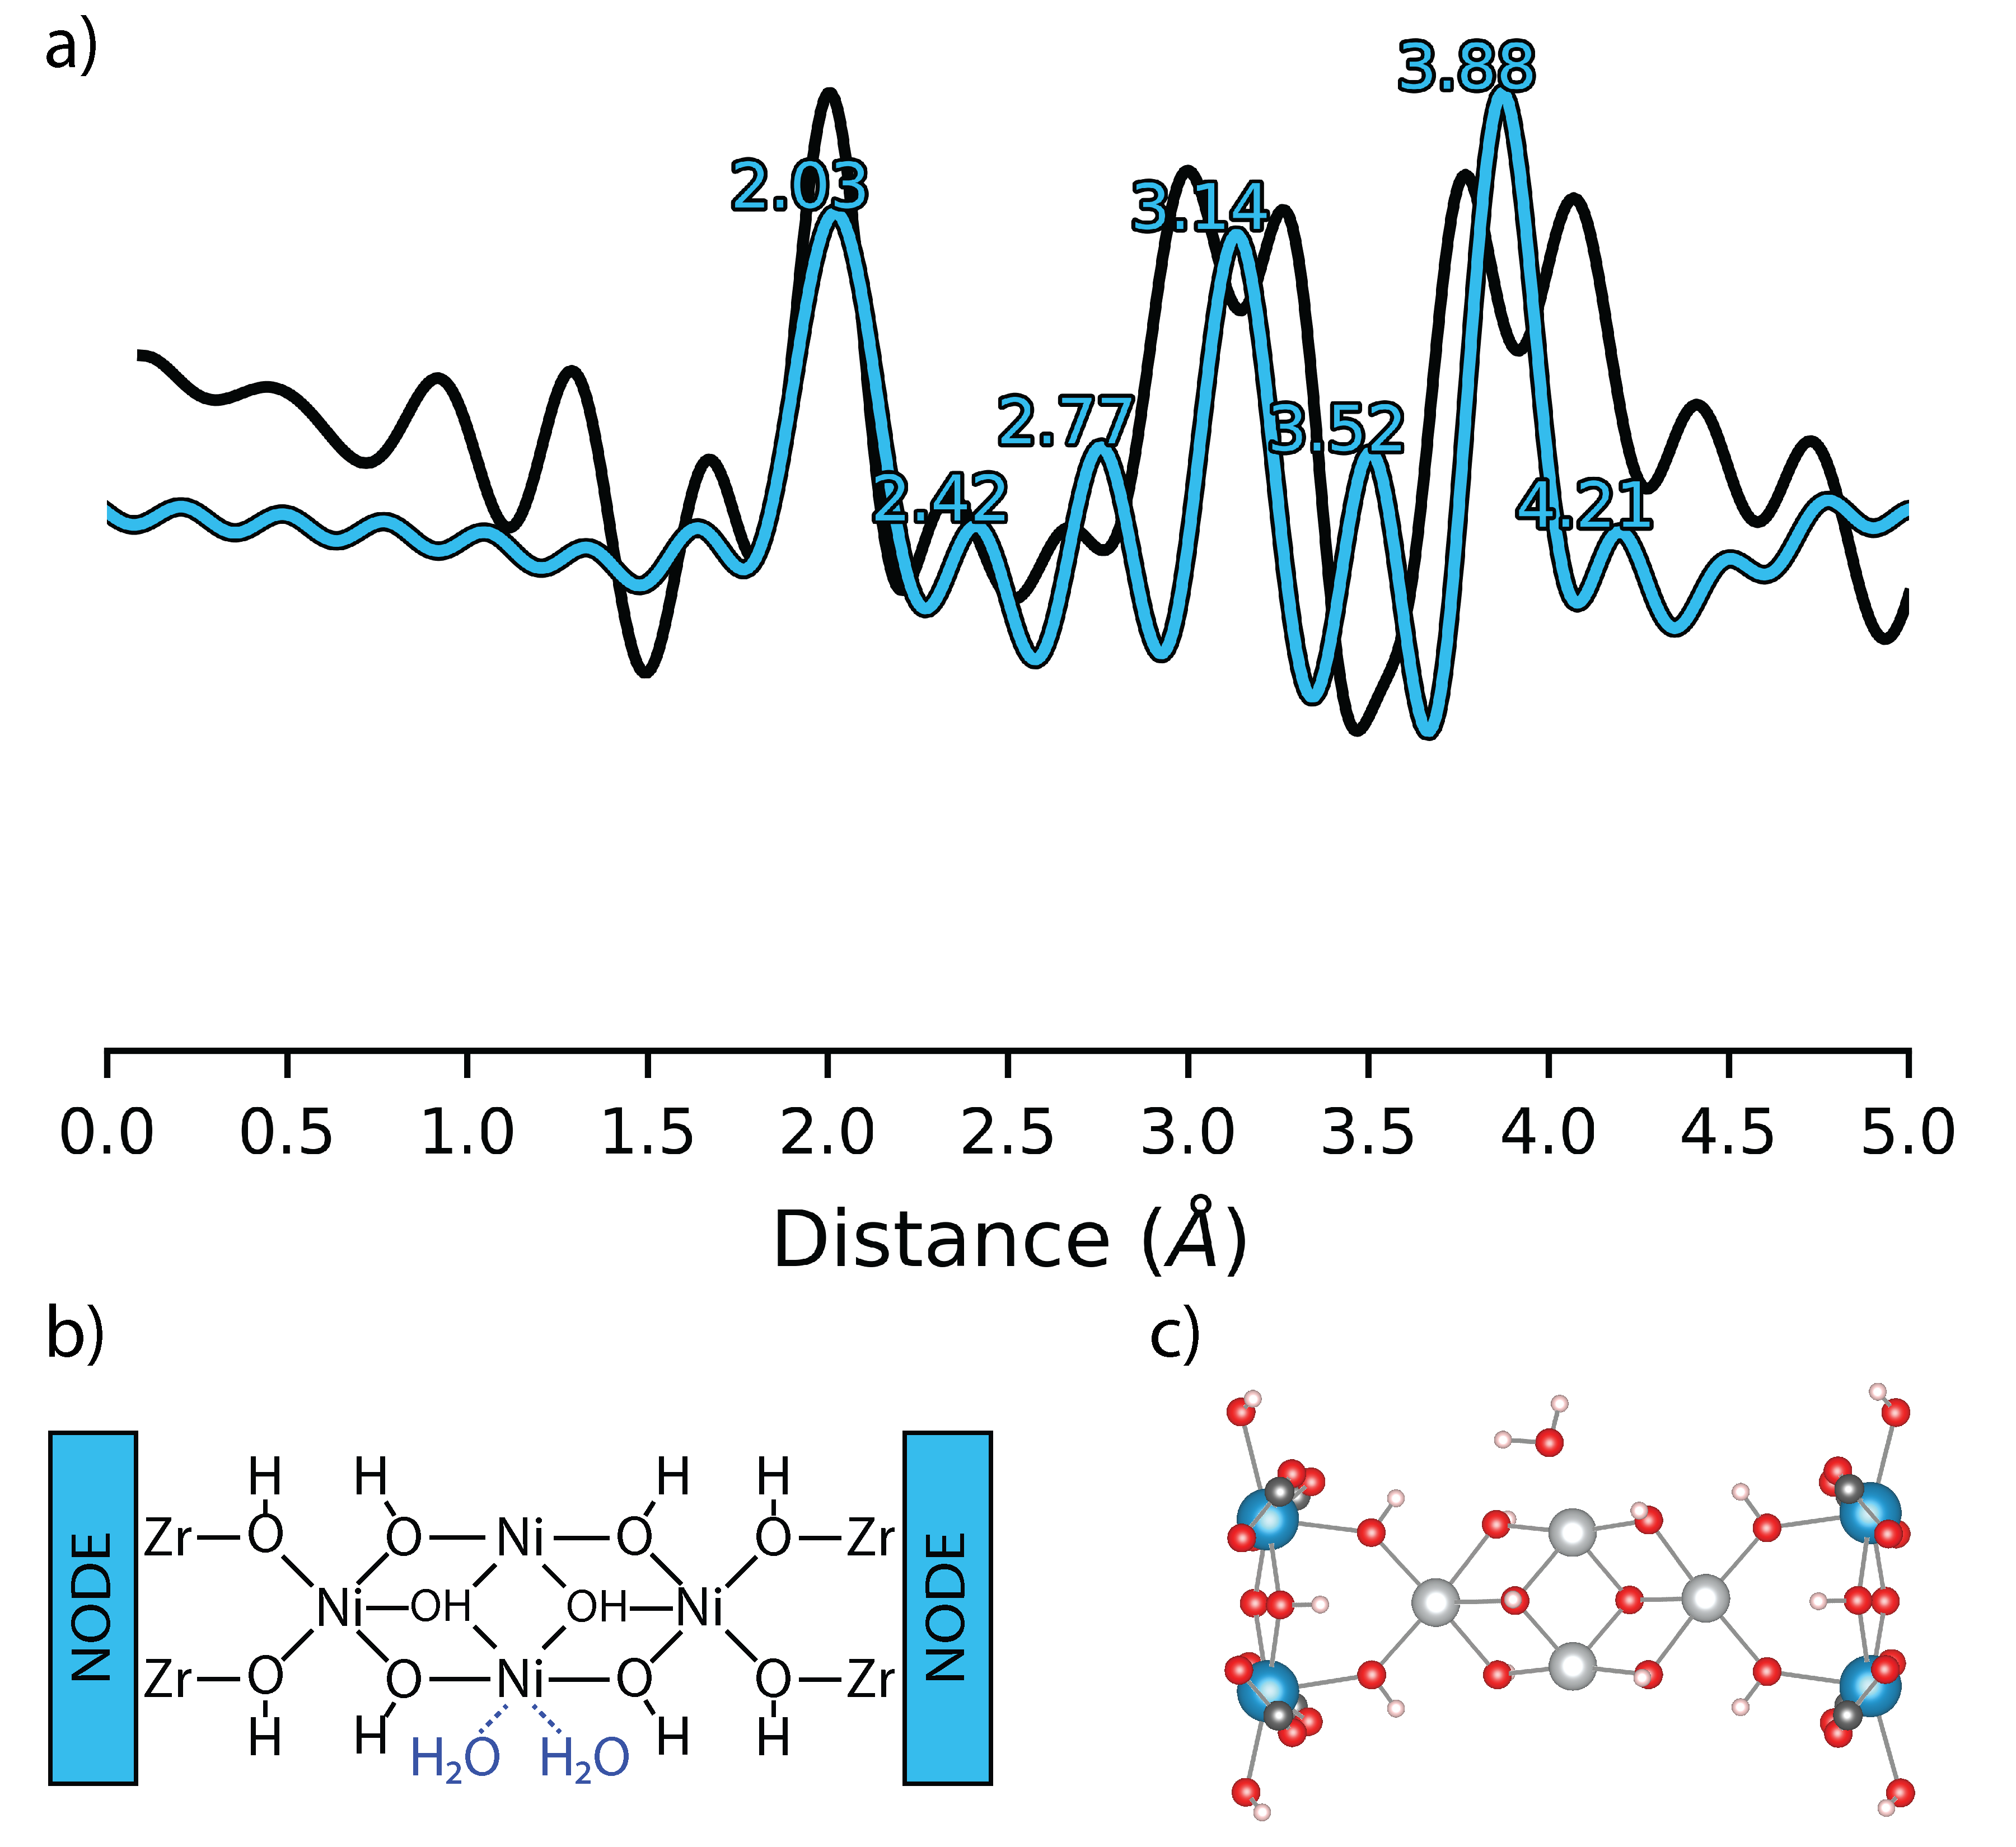
\includegraphics[width=0.75\textwidth]{zi-images/04-SI-images/SI-dPDF-Cyan.png}
    \caption{The local structural information for the \ce{Ni4(OH)6.2H2O} (cyan) structure, presented as the (a) d-PDF, (b) the schematic representation, and (c) a 3D rendering. The key distances for \ce{Ni4(OH)6.2H2O} (cyan) based on d-PDF analysis include a \ce{Ni-O} peak at 2.03 {\AA}, \ce{Ni{\Compactcdots}Ni} peaks at 2.77 and 3.14 {\AA}, and a  \ce{Ni{\Compactcdots}Zr} peak at 3.88 {\AA}, as seen in (a). The structure exhibits split \ce{Ni{\Compactcdots}Ni} peaks that do not match the experimental d-PDF.
    }
    \label{fig:SI-dPDF-cyan}
\end{figure}
    
\begin{figure}[H]
    \centering
    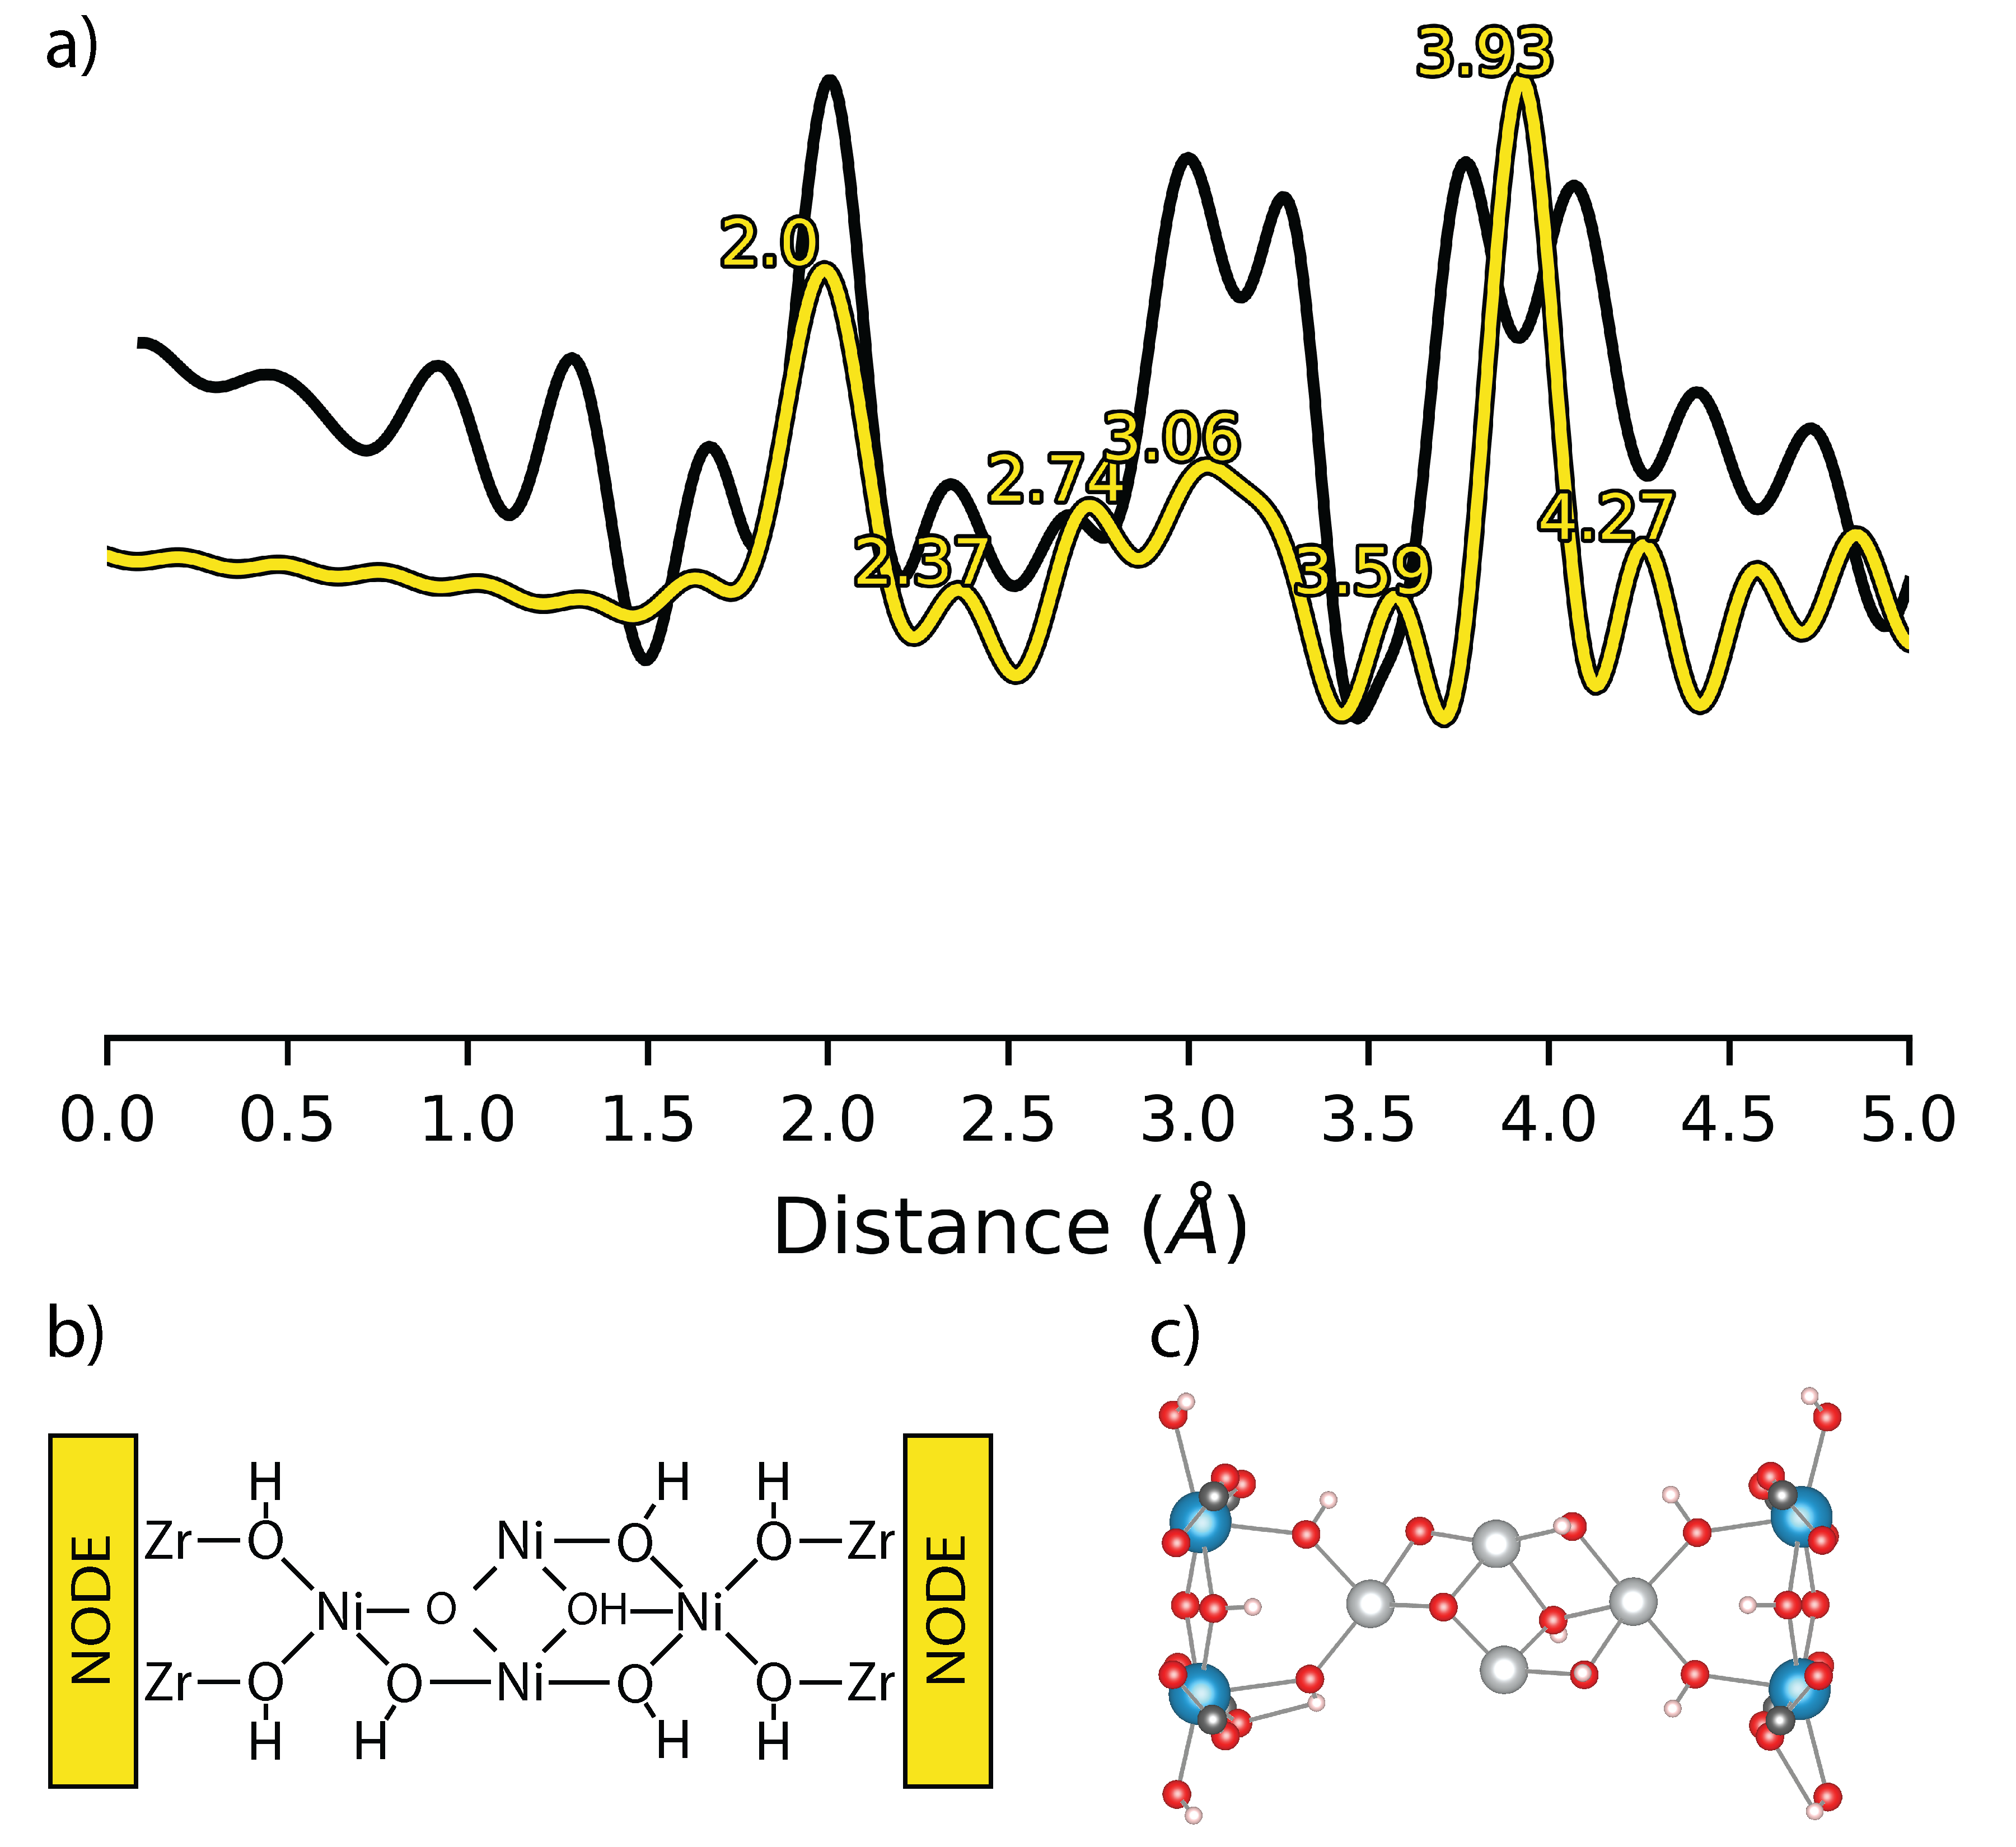
\includegraphics[width=0.75\textwidth]{zi-images/04-SI-images/SI-dPDF-Yellow.png}
    \caption{The local structural information for the \ce{Ni4(OH)4(O)} (yellow) structure, presented as the (a) d-PDF, (b) the schematic representation, and (c) a 3D rendering. The key distances for \ce{Ni4(OH)4(O)} (yellow) based on d-PDF analysis include a \ce{Ni-O} peak at 2.00 {\AA}, \ce{Ni{\Compactcdots}Ni} peaks at 2.74 and 3.06 {\AA}, and \ce{Ni{\Compactcdots}Zr} peaks at 3.93 {\AA}, as seen in (a). The split \ce{Ni{\Compactcdots}Ni} peaks are not as pronounced as other structures, with the peaks being broad. 
    }
    \label{fig:SI-dPDF-yellow}
\end{figure}

\begin{figure}[H]
    \centering
    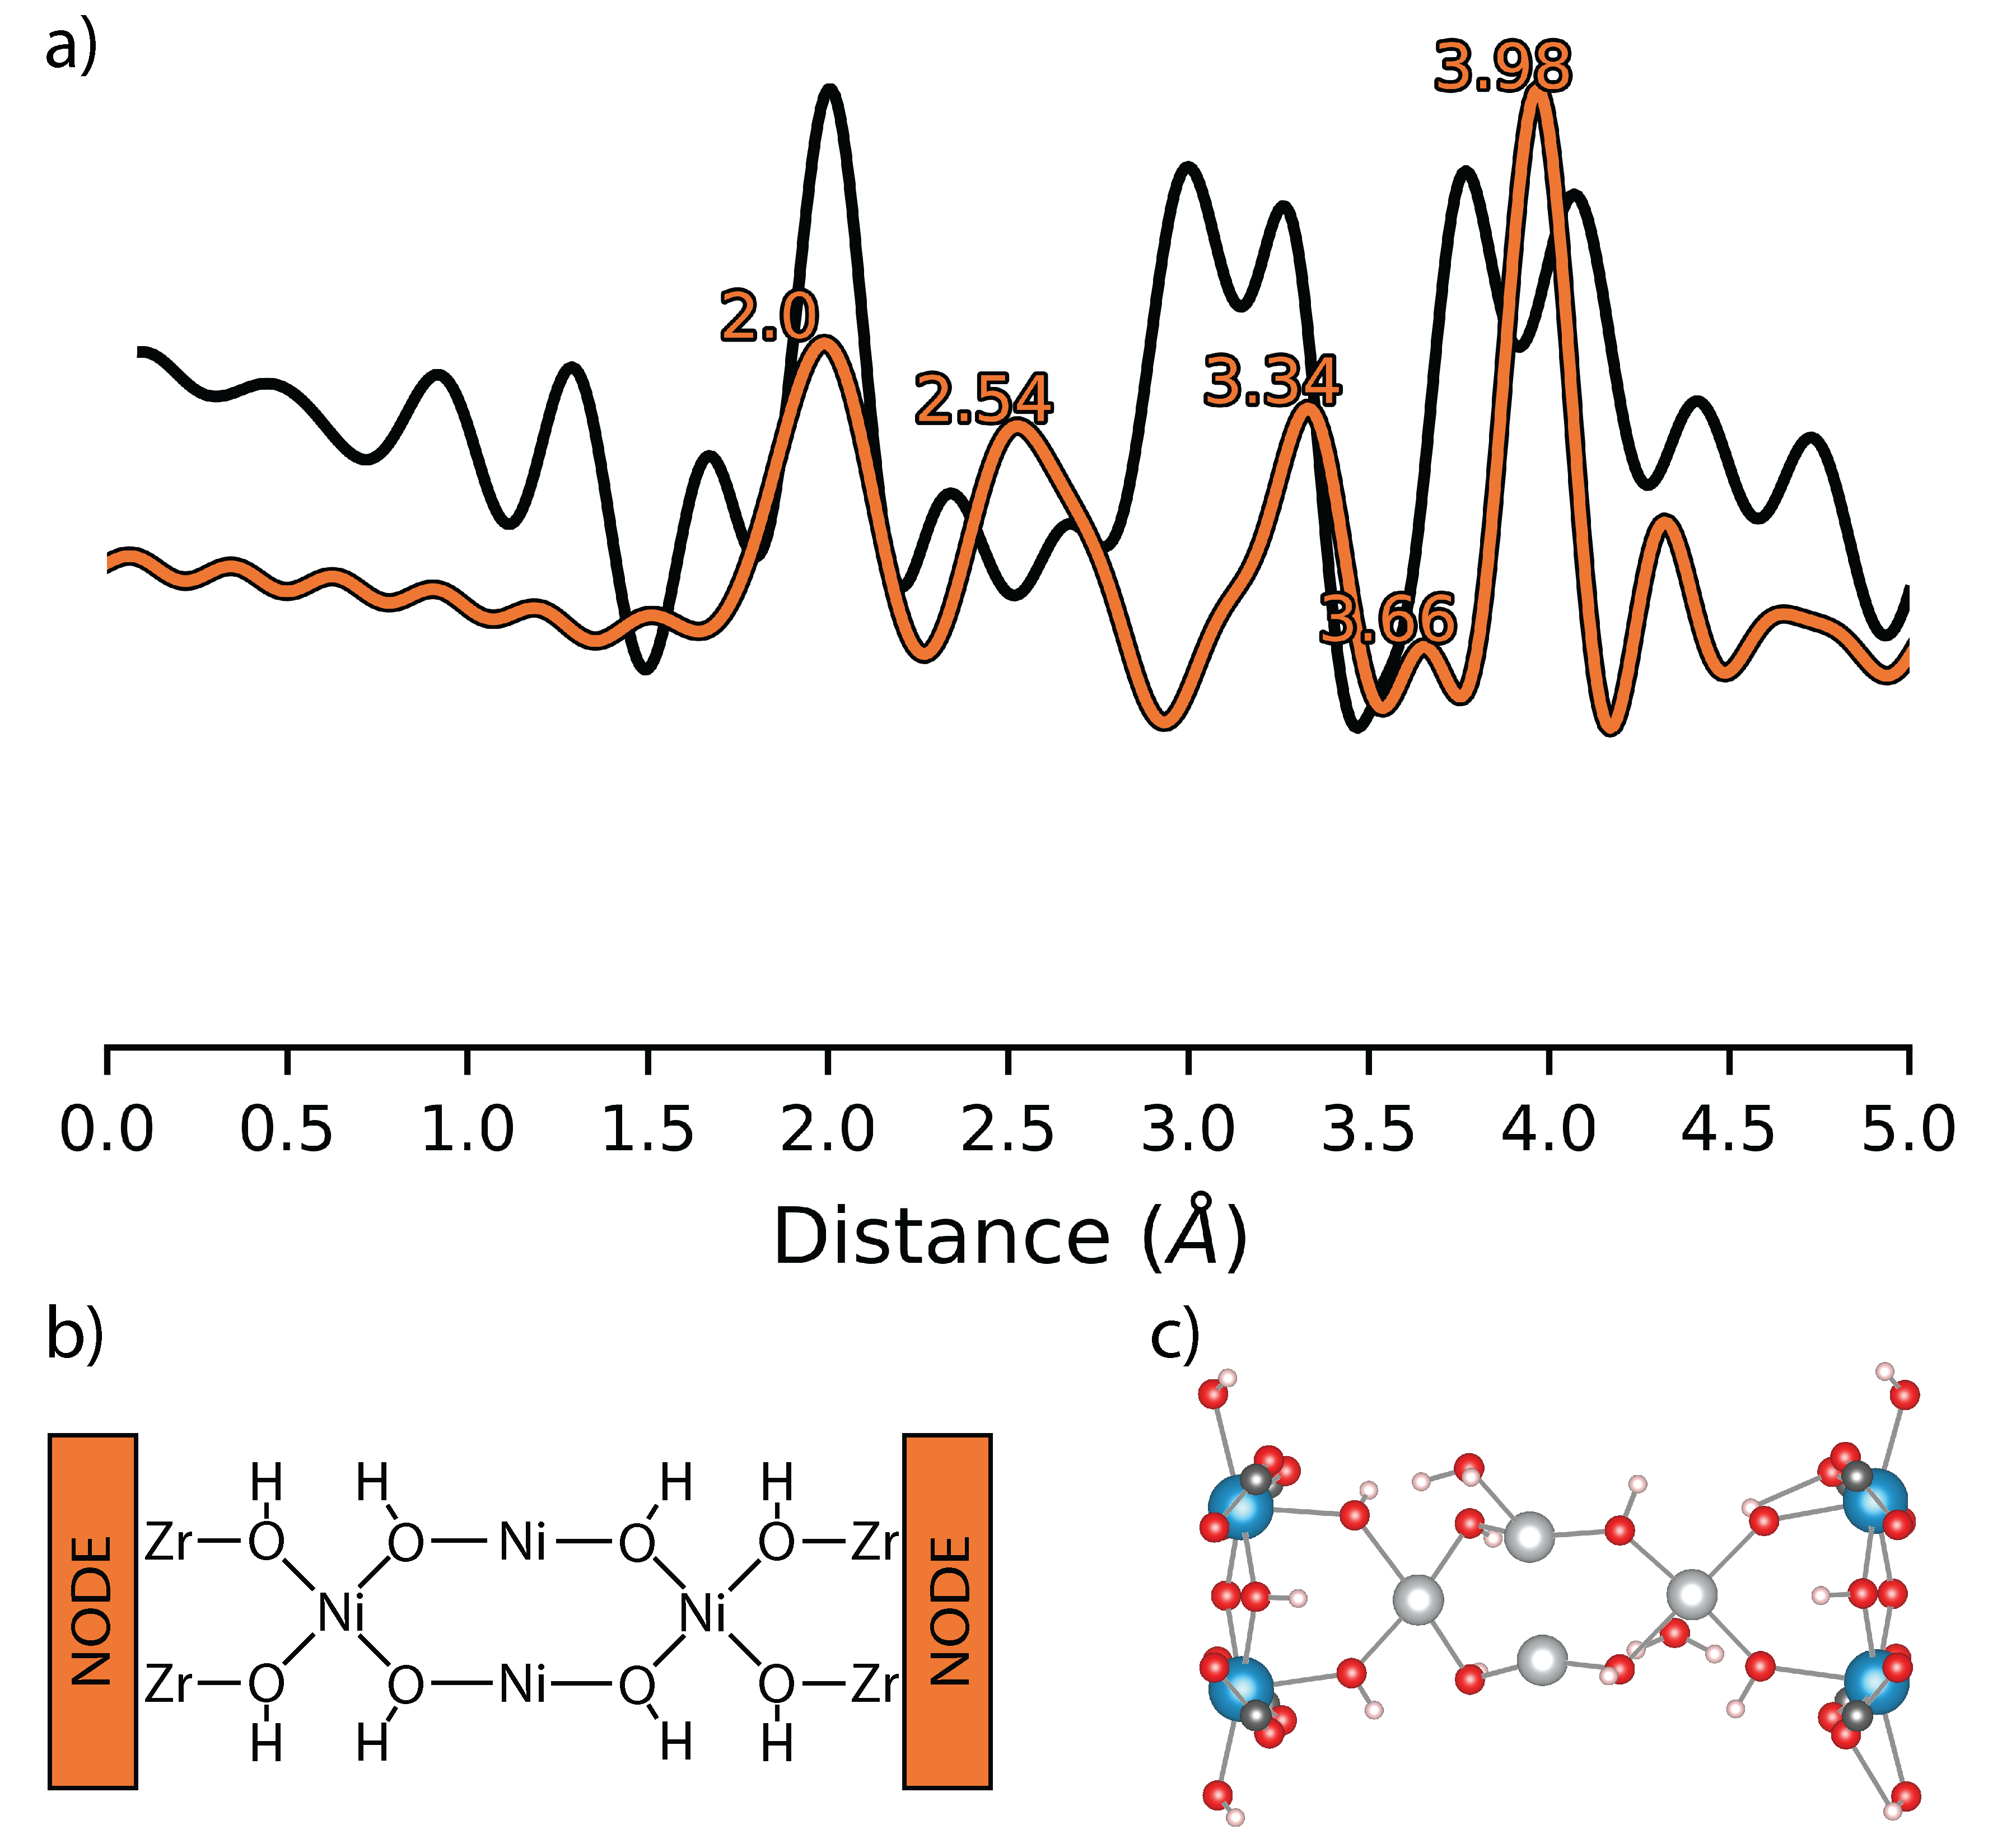
\includegraphics[width=0.75\textwidth]{zi-images/04-SI-images/SI-dPDF-Orange.png}
    \caption{The local structural information for the \ce{Ni4(OH)4.2H2O} (orange) structure, presented as the (a) d-PDF, (b) the schematic representation, and (c) a 3D rendering. The key distances for \ce{Ni4(OH)4.2H2O} (orange) based on d-PDF analysis include a \ce{Ni-O} peak at 2.02 {\AA}, \ce{Ni{\Compactcdots}Ni} peaks at 2.54 and 3.34 {\AA}, and a  \ce{Ni{\Compactcdots}Zr} peak at 3.98 {\AA}, as seen in (a). The peak at 2.54 {\AA} is from the middle \ce{Ni} ions having a low \ce{Ni-O} coordination number. 
    }
    \label{fig:SI-dPDF-orange}
\end{figure}

\begin{figure}[H]
    \centering
    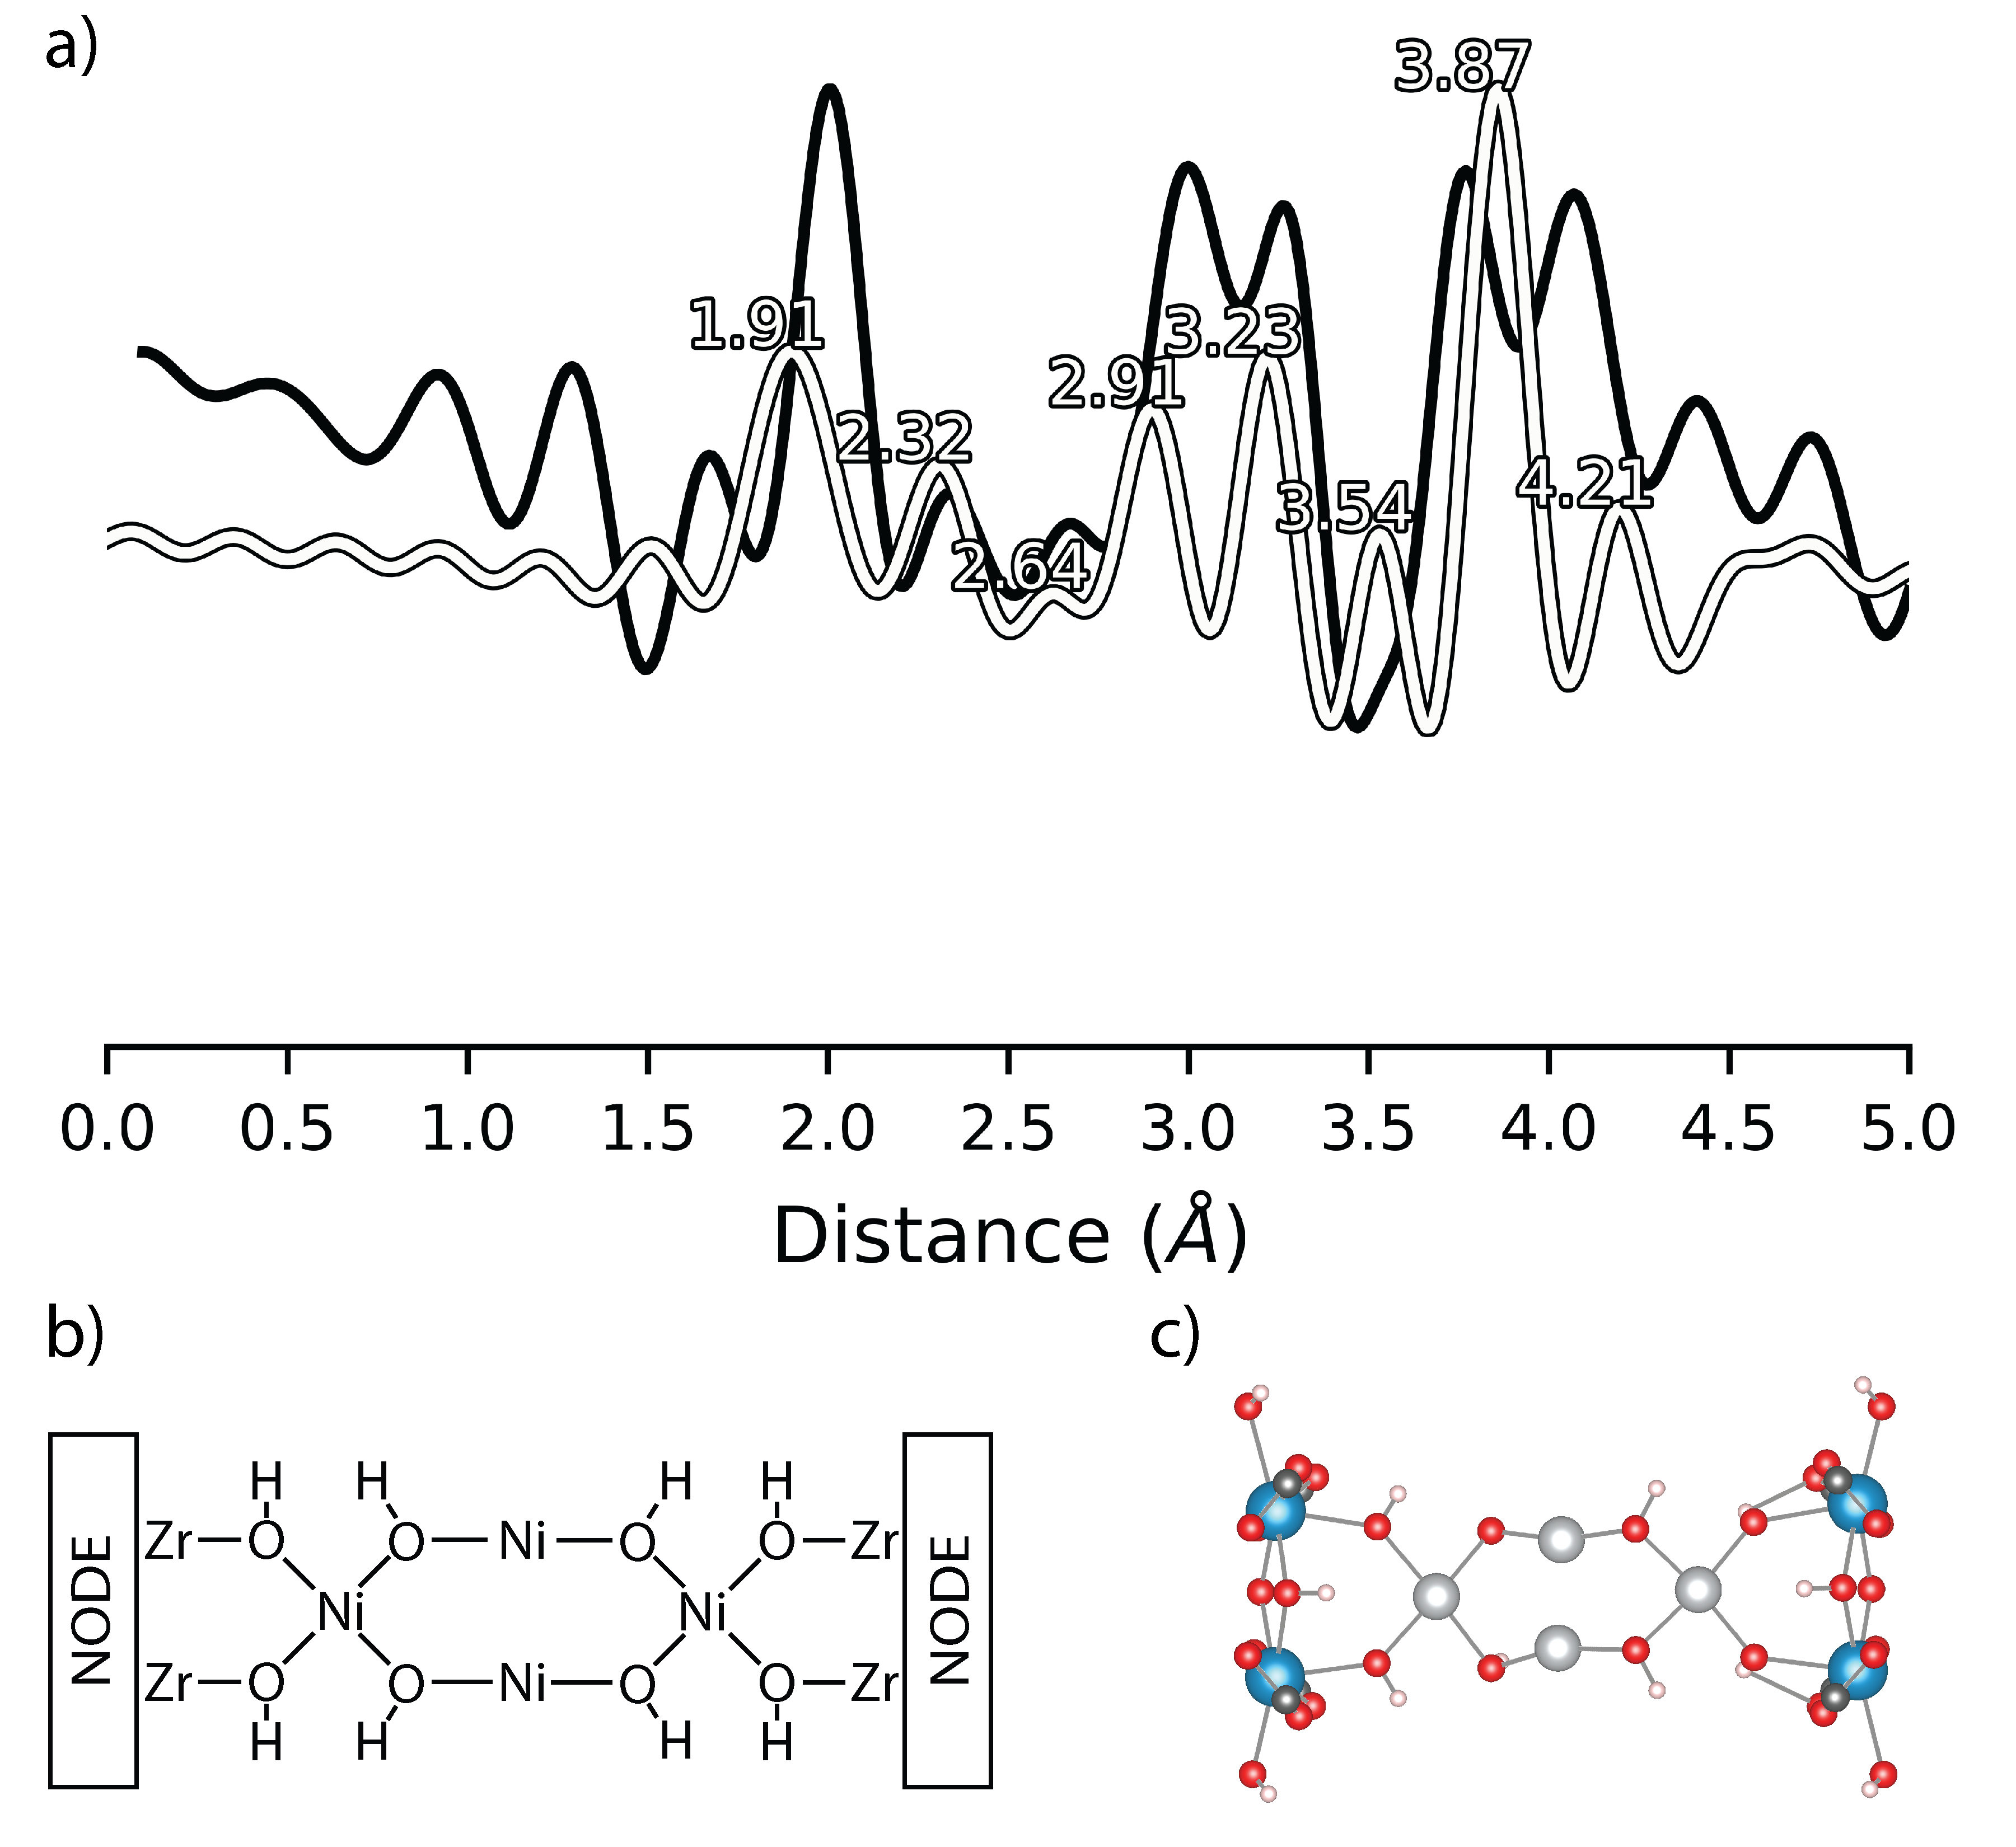
\includegraphics[width=0.75\textwidth]{zi-images/04-SI-images/SI-dPDF-White.png}
    \caption{The local structural information for the \ce{Ni4(OH)4} (white) structure, presented as the (a) d-PDF, (b) the schematic representation, and (c) a 3D rendering. The key distances for \ce{Ni4(OH)4} (white) based on d-PDF analysis include a \ce{Ni-O} peak at 1.91 {\AA}, \ce{Ni{\Compactcdots}Ni} peaks at 2.32, 2.91, and 3.23 {\AA}, and \ce{Ni{\Compactcdots}Zr} peaks at 3.87 {\AA}, as seen in (a). The removal of both $\mu_{3}-\ce{OH}$ ligands and a lack of \ce{H2O} ligands is why a \ce{Ni{\Compactcdots}Ni} peak is observed at 2.32 {\AA}.
    }
    \label{fig:SI-dPDF-white}
\end{figure}

\begin{figure}[H]
    \centering
    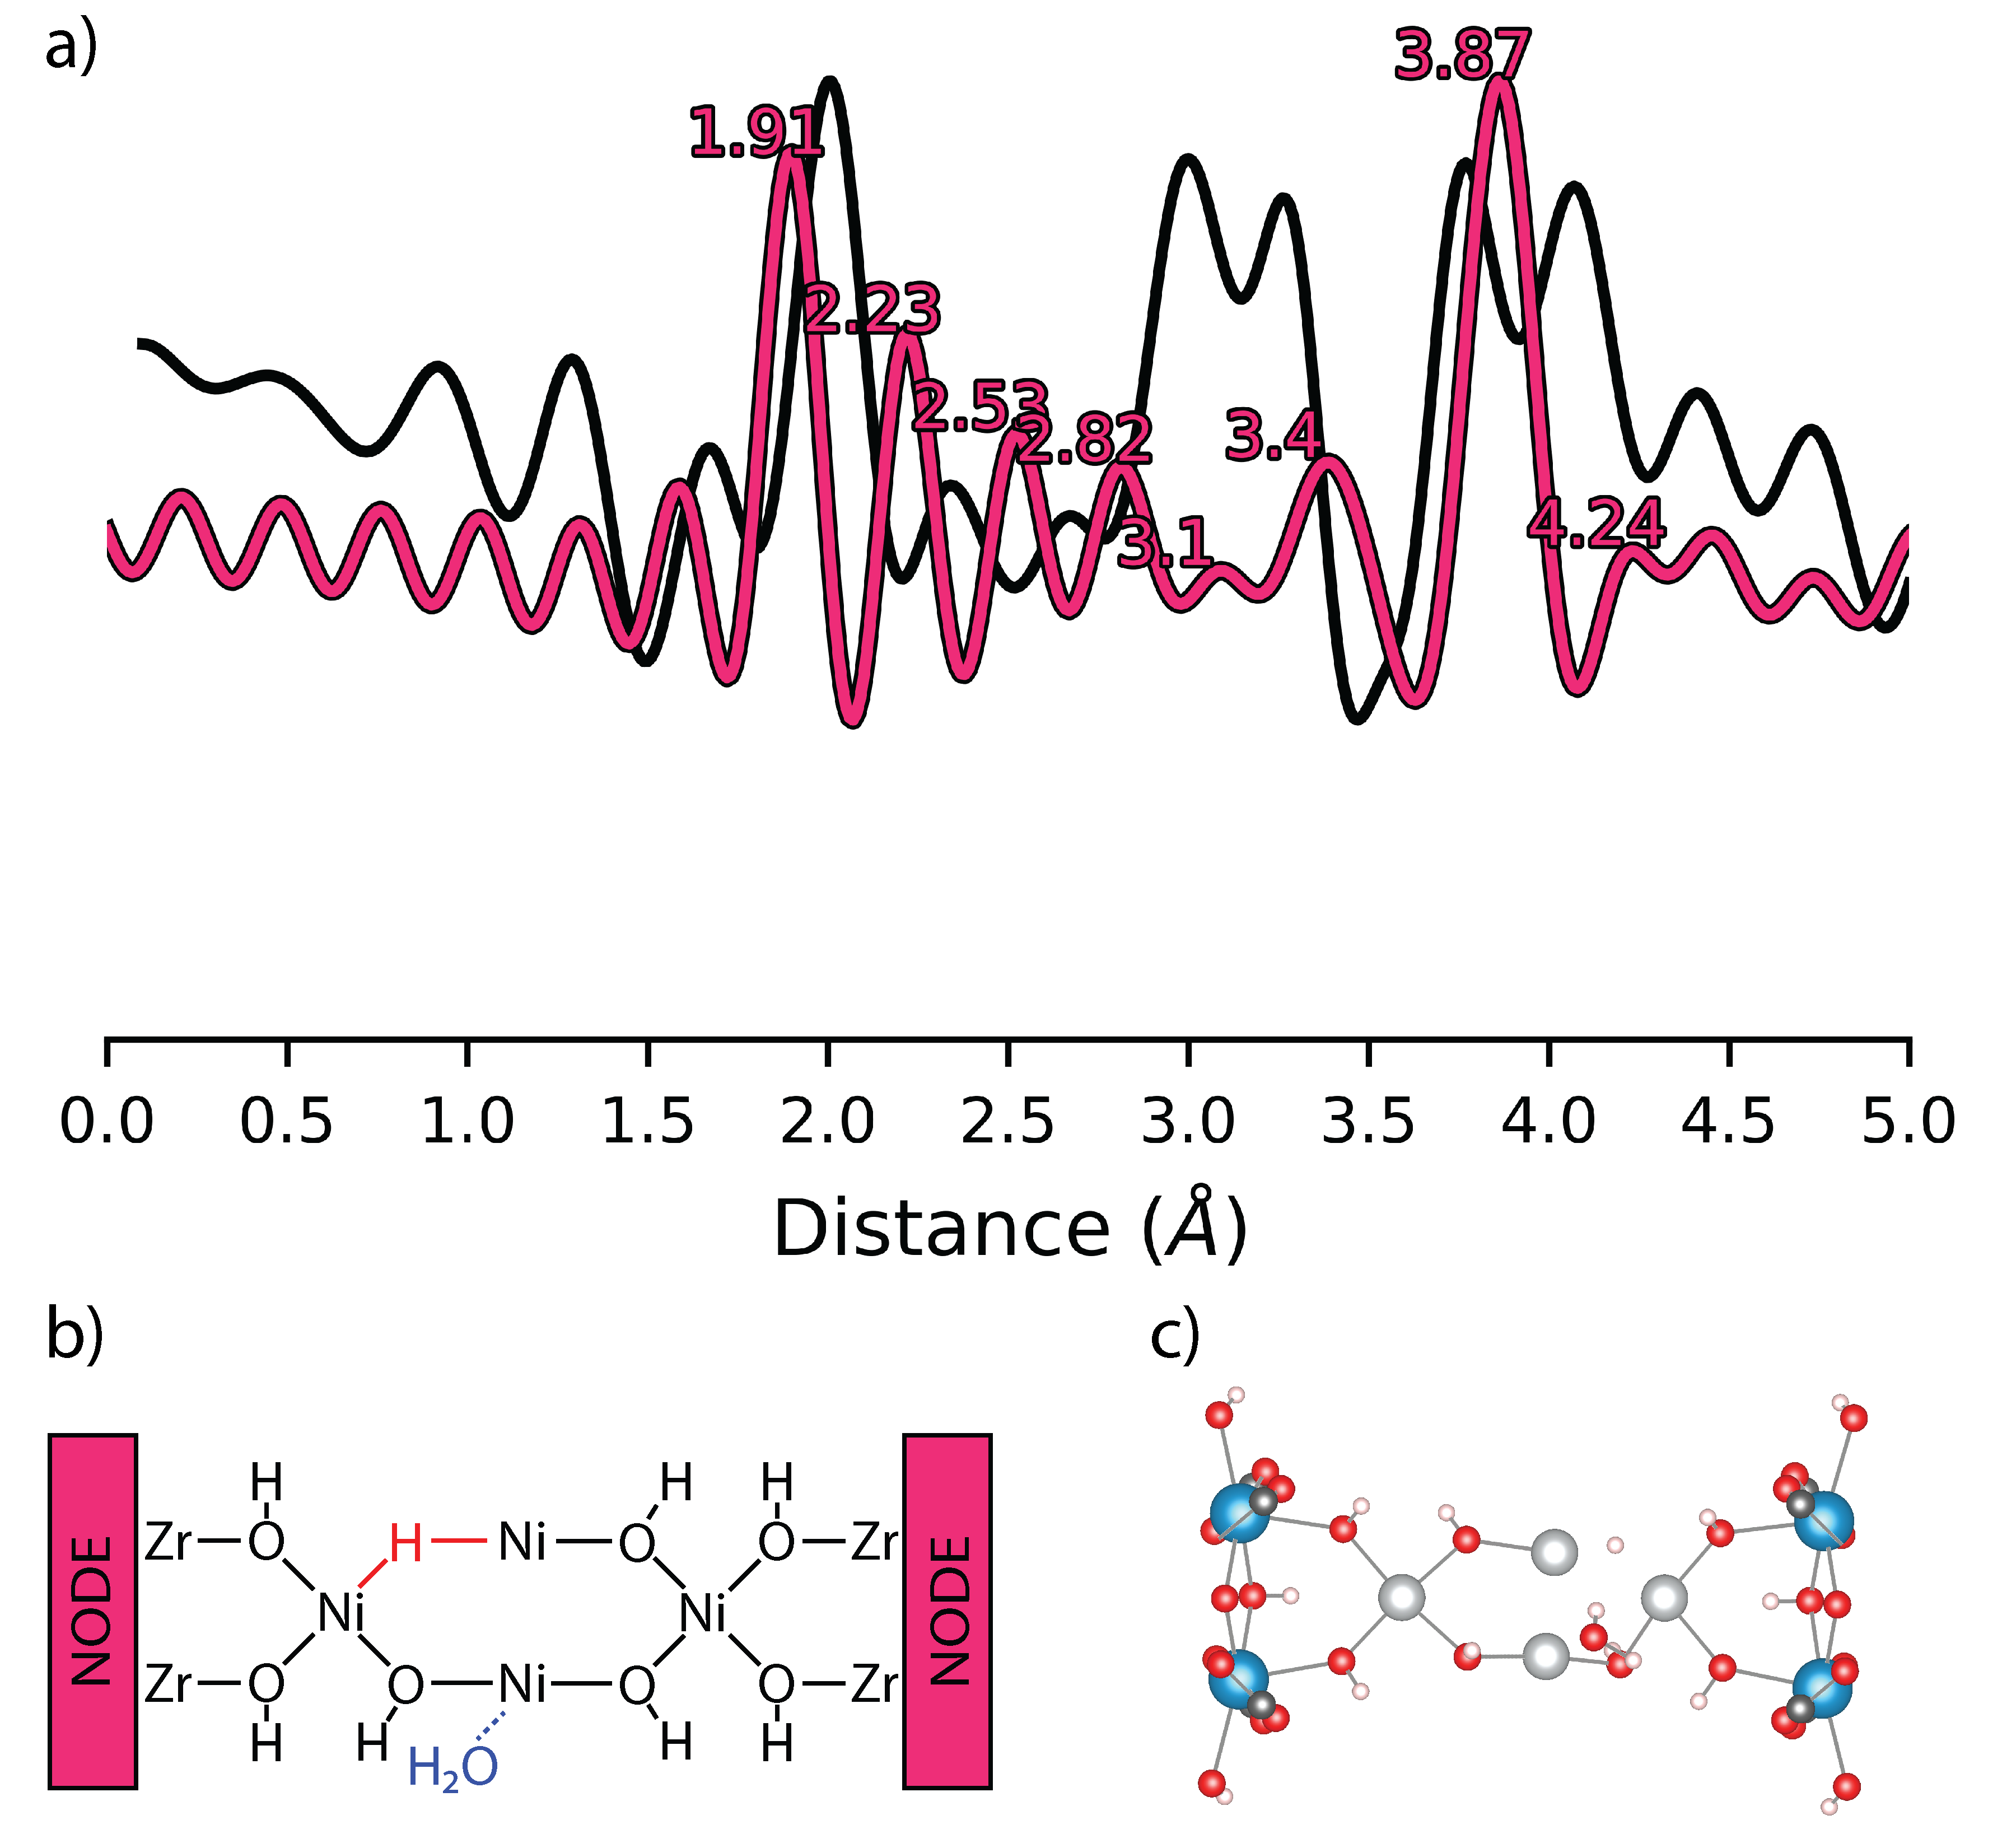
\includegraphics[width=0.75\textwidth]{zi-images/04-SI-images/SI-dPDF-Magenta.png}
    \caption{The local structural information for the \ce{Ni4(OH)3(H).H2O} (magenta) structure, presented as the (a) d-PDF, (b) the schematic representation, and (c) a 3D rendering. The key distances for \ce{Ni4(OH)3(H).H2O} (magenta)  based on d-PDF analysis include \ce{Ni-O} peak at 1.91 {\AA}, \ce{Ni{\Compactcdots}Ni} peaks at 2.23, 2.53, 2.82, and 3.40 {\AA}, and a \ce{Ni{\Compactcdots}Zr} peak at 3.87 {\AA}, as seen in (a). 
    }
    \label{fig:SI-dPDF-magneta}
\end{figure}

\begin{figure}[H]
    \centering
    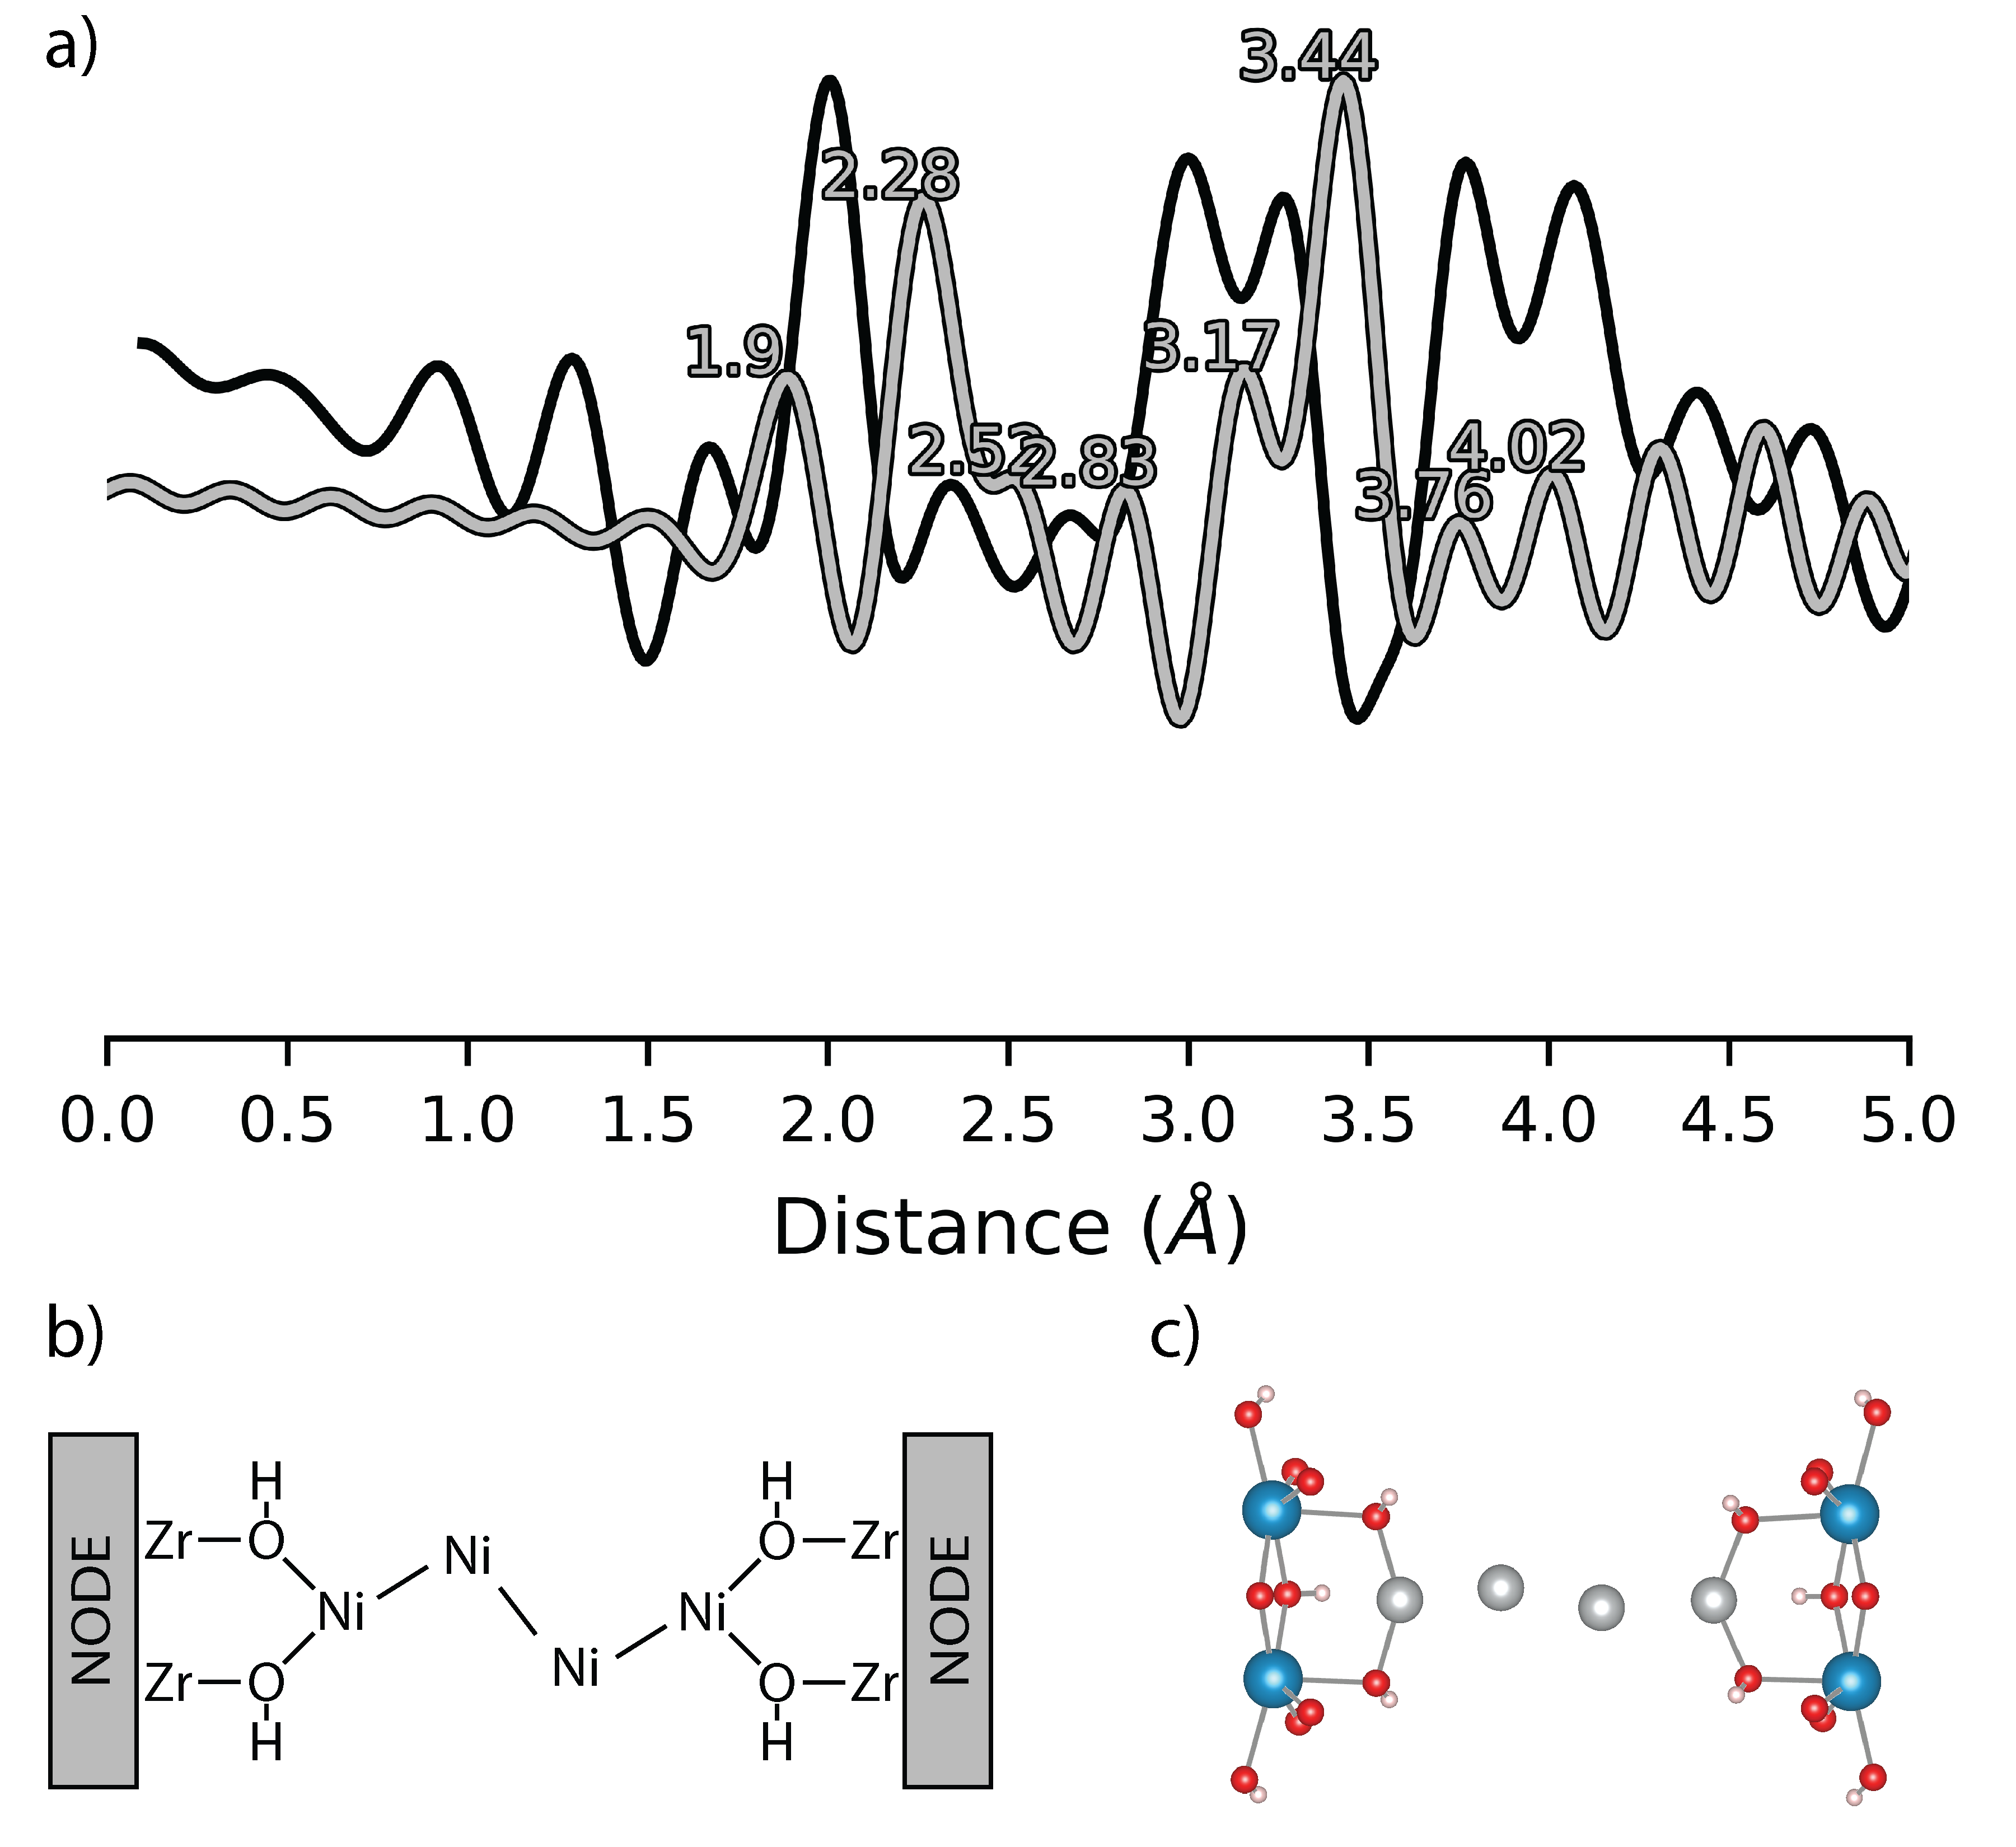
\includegraphics[width=0.75\textwidth]{zi-images/04-SI-images/SI-dPDF-Gray.png}
    \caption{
        The local structural information for the \ce{Ni4} (gray) structure, presented as the (a) d-PDF, (b) the schematic representation, and (c) a 3D rendering. The key distances for \ce{Ni4} (gray) based on d-PDF analysis include the \ce{Ni-O} peak at 1.9 {\AA}, the \ce{Ni{\Compactcdots}Ni} peak at 2.28 {\AA}, and the \ce{Ni{\Compactcdots}Zr} peak at 3.44 {\AA}.
    }
    \label{fig:SI-dPDF-gray}
\end{figure}
    
\begin{figure}[H]
    \centering
    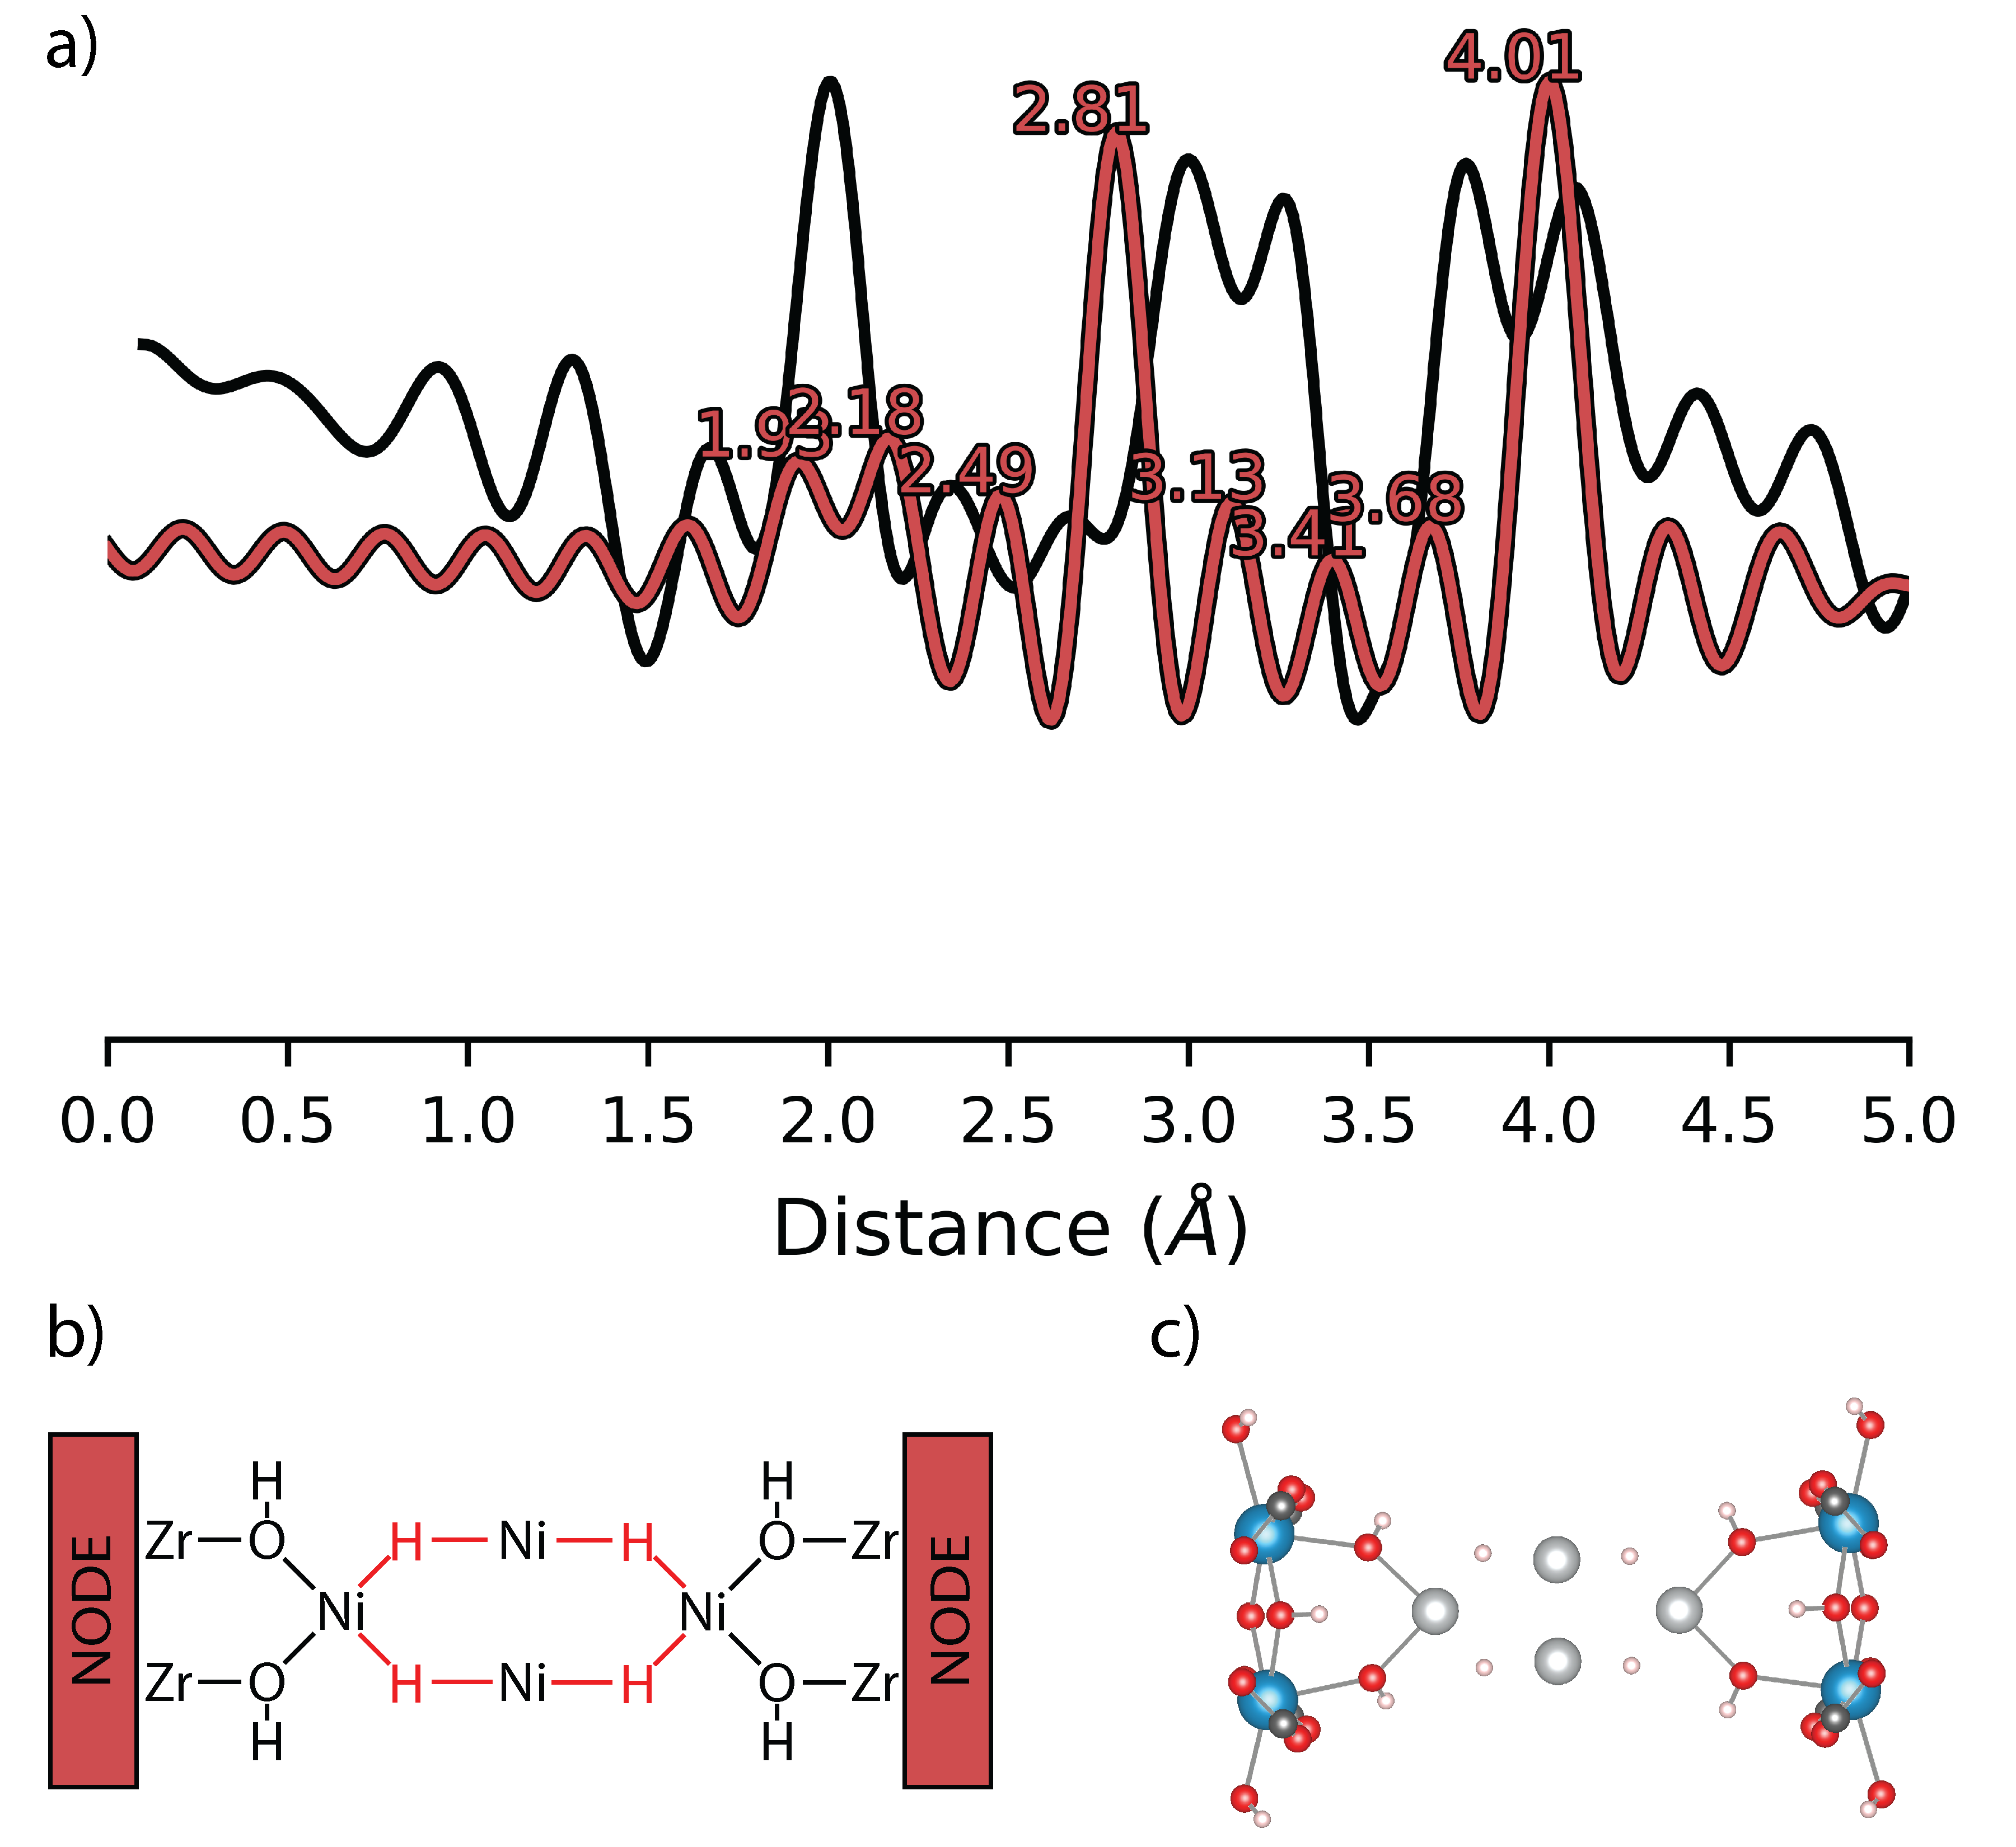
\includegraphics[width=0.75\textwidth]{zi-images/04-SI-images/SI-dPDF-Red.png}
    \caption{
        The local structural information for the \ce{Ni4(H)4} (red) structure, presented as the (a) d-PDF, (b) the schematic representation, and (c) a 3D rendering. The key distances for \ce{Ni4(H)4} (red) based on d-PDF analysis include \ce{Ni-O} peak at 1.93 {\AA}, \ce{Ni{\Compactcdots}Ni} peaks at 2.18 and 2.81 {\AA}, and \ce{Ni{\Compactcdots}Zr} peaks at 4.01 {\AA}, as seen in (a). All of the \ce{Ni} feature a \ce{Ni-H-Ni} motif, which forces the middle \ce{Ni} ions to be closer together (hence the peak at 2.18 {\AA}).
    }
    \label{fig:SI-dPDF-red}
\end{figure}


%%%%%%%%%%%%%%%%%%%%%%%%%%%%%%%%%%%%%%%%%%%%%%%%%%%%%%%%%%%%%%%%%%%%%
%% Key alternate structures
%%%%%%%%%%%%%%%%%%%%%%%%%%%%%%%%%%%%%%%%%%%%%%%%%%%%%%%%%%%%%%%%%%%%%
\newpage
\section{Key alternate structures}
Additionally, we identified key alternate structures that are not thermodynamic minima according to \textit{ab initio} thermodynamic analysis. These structures are shown in Figures~S\ref{fig:SI-dPDF-teal} and~S\ref{fig:SI-dPDF-maroon}. Each figure includes the (a) d-PDF, (b) the schematic drawing, and (c) the atomic rendering for that structure. 

\begin{figure}[H]
    \centering
    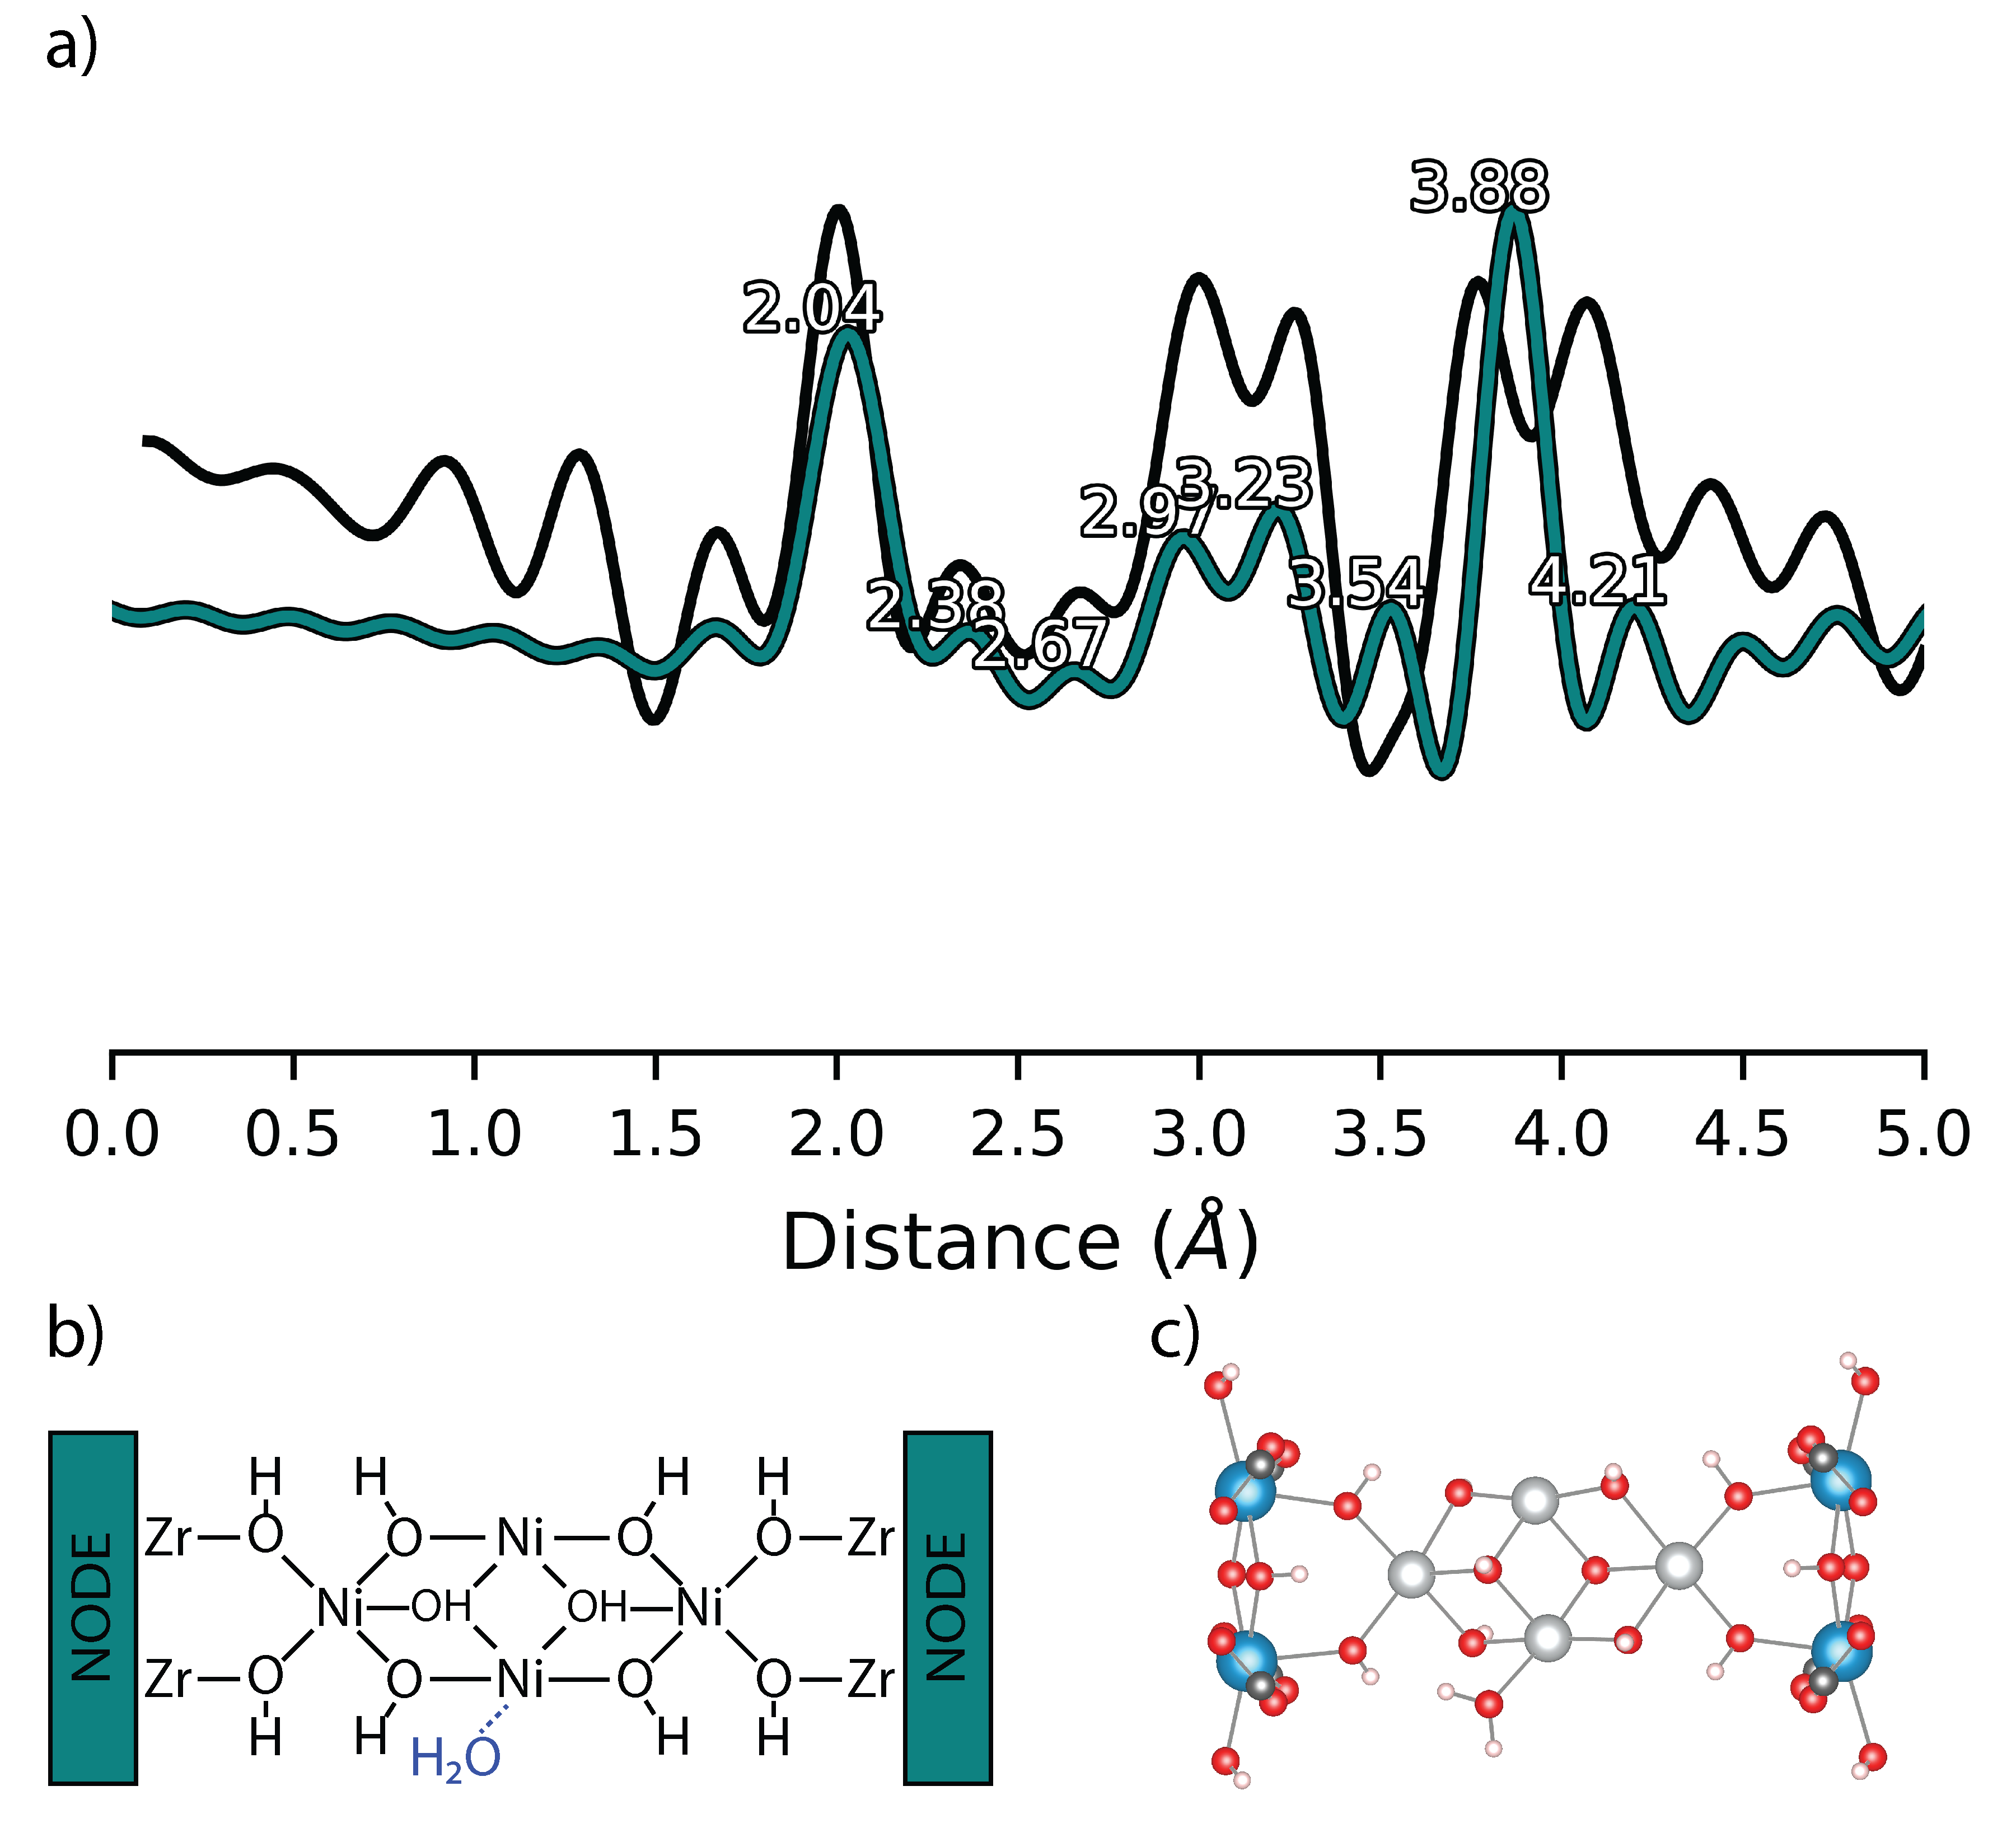
\includegraphics[width=0.75\textwidth]{zi-images/04-SI-images/SI-dPDF-Teal.png}
    \caption{
        The local structural information for the \ce{Ni4(OH)6.1H2O} (teal) structure, presented as the (a) d-PDF, (b) the schematic representation, and (c) a 3D rendering. The key distances for \ce{Ni4(OH)6.1H2O} (teal) based on d-PDF analysis include \ce{Ni-O} peak at 2.04 {\AA}, \ce{Ni{\Compactcdots}Ni} peaks at 2.97 and 3.23 {\AA}, and \ce{Ni{\Compactcdots}Zr} peaks at 3.88 {\AA}, as seen in (a).
    }
    \label{fig:SI-dPDF-teal}
\end{figure}

\begin{figure}[H]
    \centering
    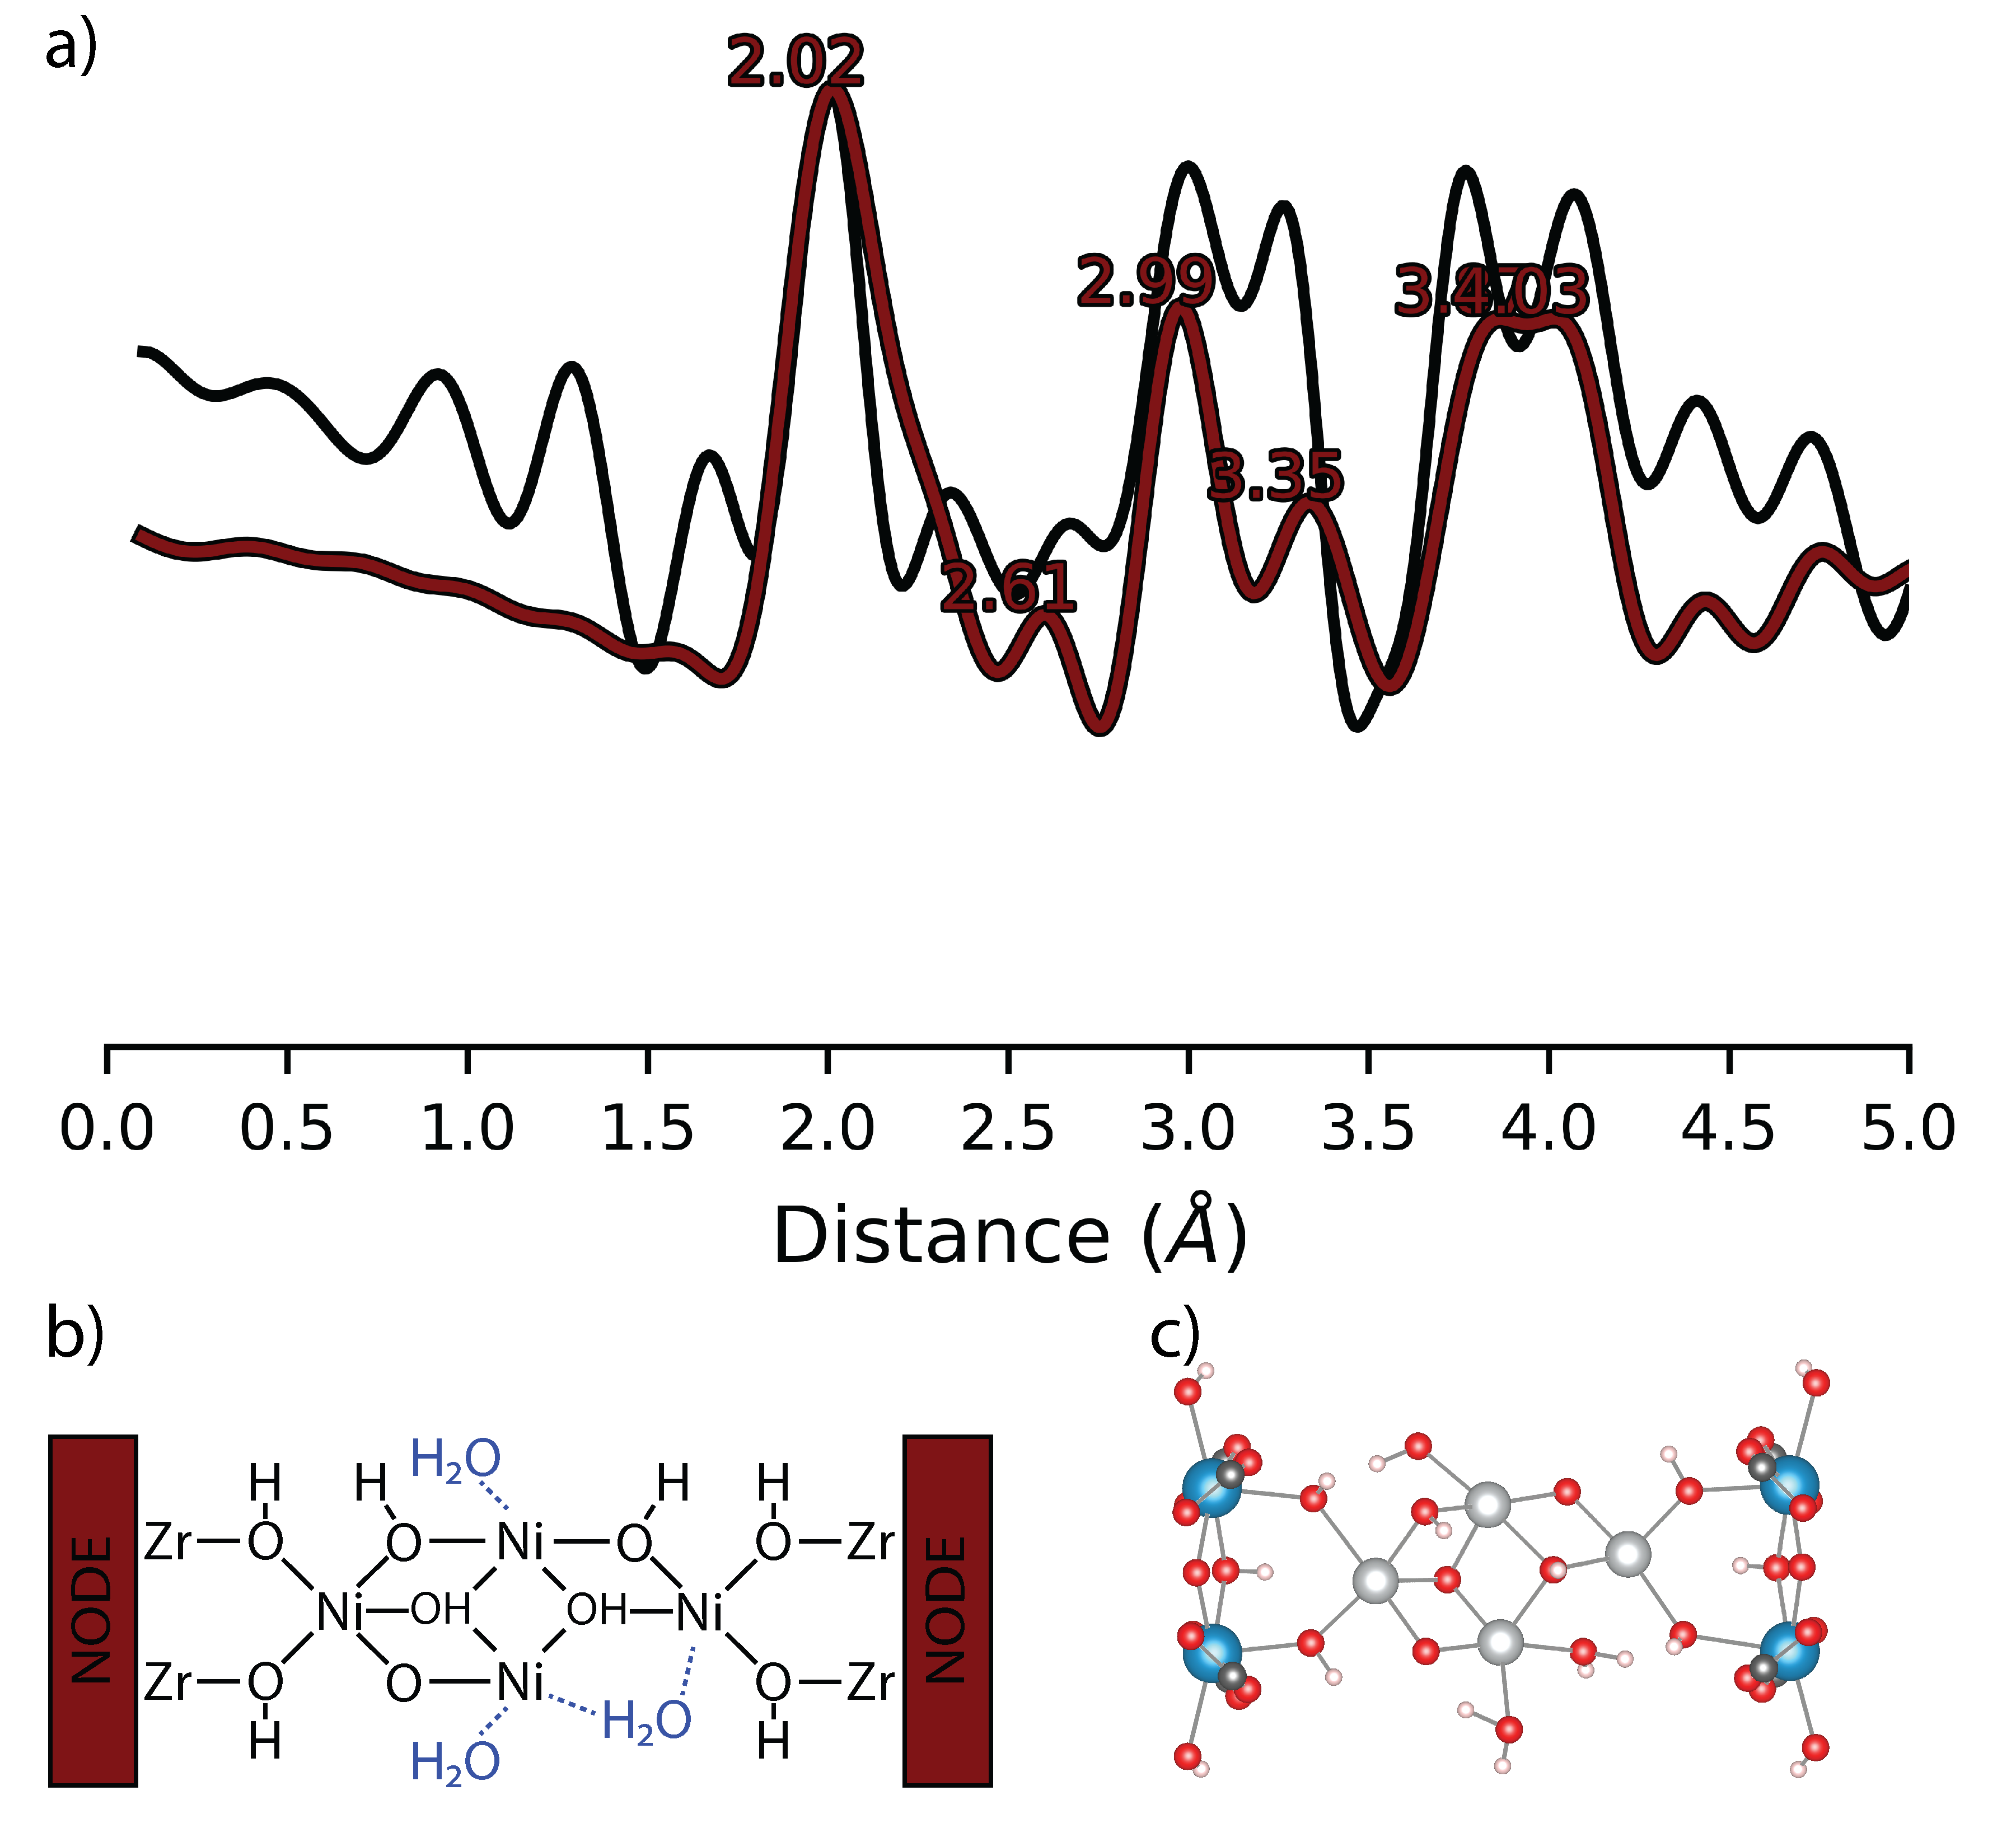
\includegraphics[width=0.75\textwidth]{zi-images/04-SI-images/SI-dPDF-Maroon.png}
    \caption{
        The local structural information for the \ce{Ni4(OH)4(O).3H2O} (maroon) structure, presented as the (a) d-PDF, (b) the schematic representation, and (c) a 3D rendering. The key distances for \ce{Ni4(OH)4(O).3H2O} (maroon) based on d-PDF analysis include \ce{Ni-O} peak at 2.02 {\AA}, \ce{Ni{\Compactcdots}Ni} peaks at 2.99 and 3.35 {\AA}, and a broadening of the \ce{Ni{\Compactcdots}Zr} peaks 3.87 and 4.03 {\AA}, as seen in (a).
    }
    \label{fig:SI-dPDF-maroon}
\end{figure}

%%%%%%%%%%%%%%%%%%%%%%%%%%%%%%%%%%%%%%%%%%%%%%%%%%%%%%%%%%%%%%%%%%%%%
%% Weighted d-PDFs
%%%%%%%%%%%%%%%%%%%%%%%%%%%%%%%%%%%%%%%%%%%%%%%%%%%%%%%%%%%%%%%%%%%%%
\newpage
\section{Boltzmann Weighted d-PDFs}
We use Boltzmann weighting to combine the structural information of unique structures into a Boltzmann weighted d-PDF. We perform the Boltzmann weighting by computing the free energies of all the structures at specific \ce{H2} and \ce{H2O} chemical potentials, and then use Eq.~\ref{eq:weighted-dPDFs} to compute the Boltzmann factor ($P_{i}$) for each structure ${i}$.
\begin{equation}
    P_{i} = \frac{e^{\frac{-\Delta G_{i}}{k_{b}T}}}{\sum_{l} e^{\frac{-\Delta G_{l}}{k_{b}T}}}
    \label{eq:weighted-dPDFs}
\end{equation}
where $\Delta G$ is the free energy of structure computed according to Eq.~\ref{eq:free-energy-trans}. We assume a temperature of $T=298 \text{K}$. Note that the Boltzmann weighting considers all the d-PDFs in our library of structures; not just the structures that are thermodynamically relevant. At specific \ce{H2} and \ce{H2O} chemical potentials, we take each d-PDF intensity between 0 {\AA} and 5 {\AA} multiplied by each Boltzmann factor for each structure and then sum all the d-PDF intensities to generate the weighted d-PDF. Key weighted Boltzmann factors are shown in Figure~\ref{fig:SI-weighted-dPDFs}b-d. 

% d-PDF diagram for all thermodynamic minima
\begin{figure}[H]
    \centering
    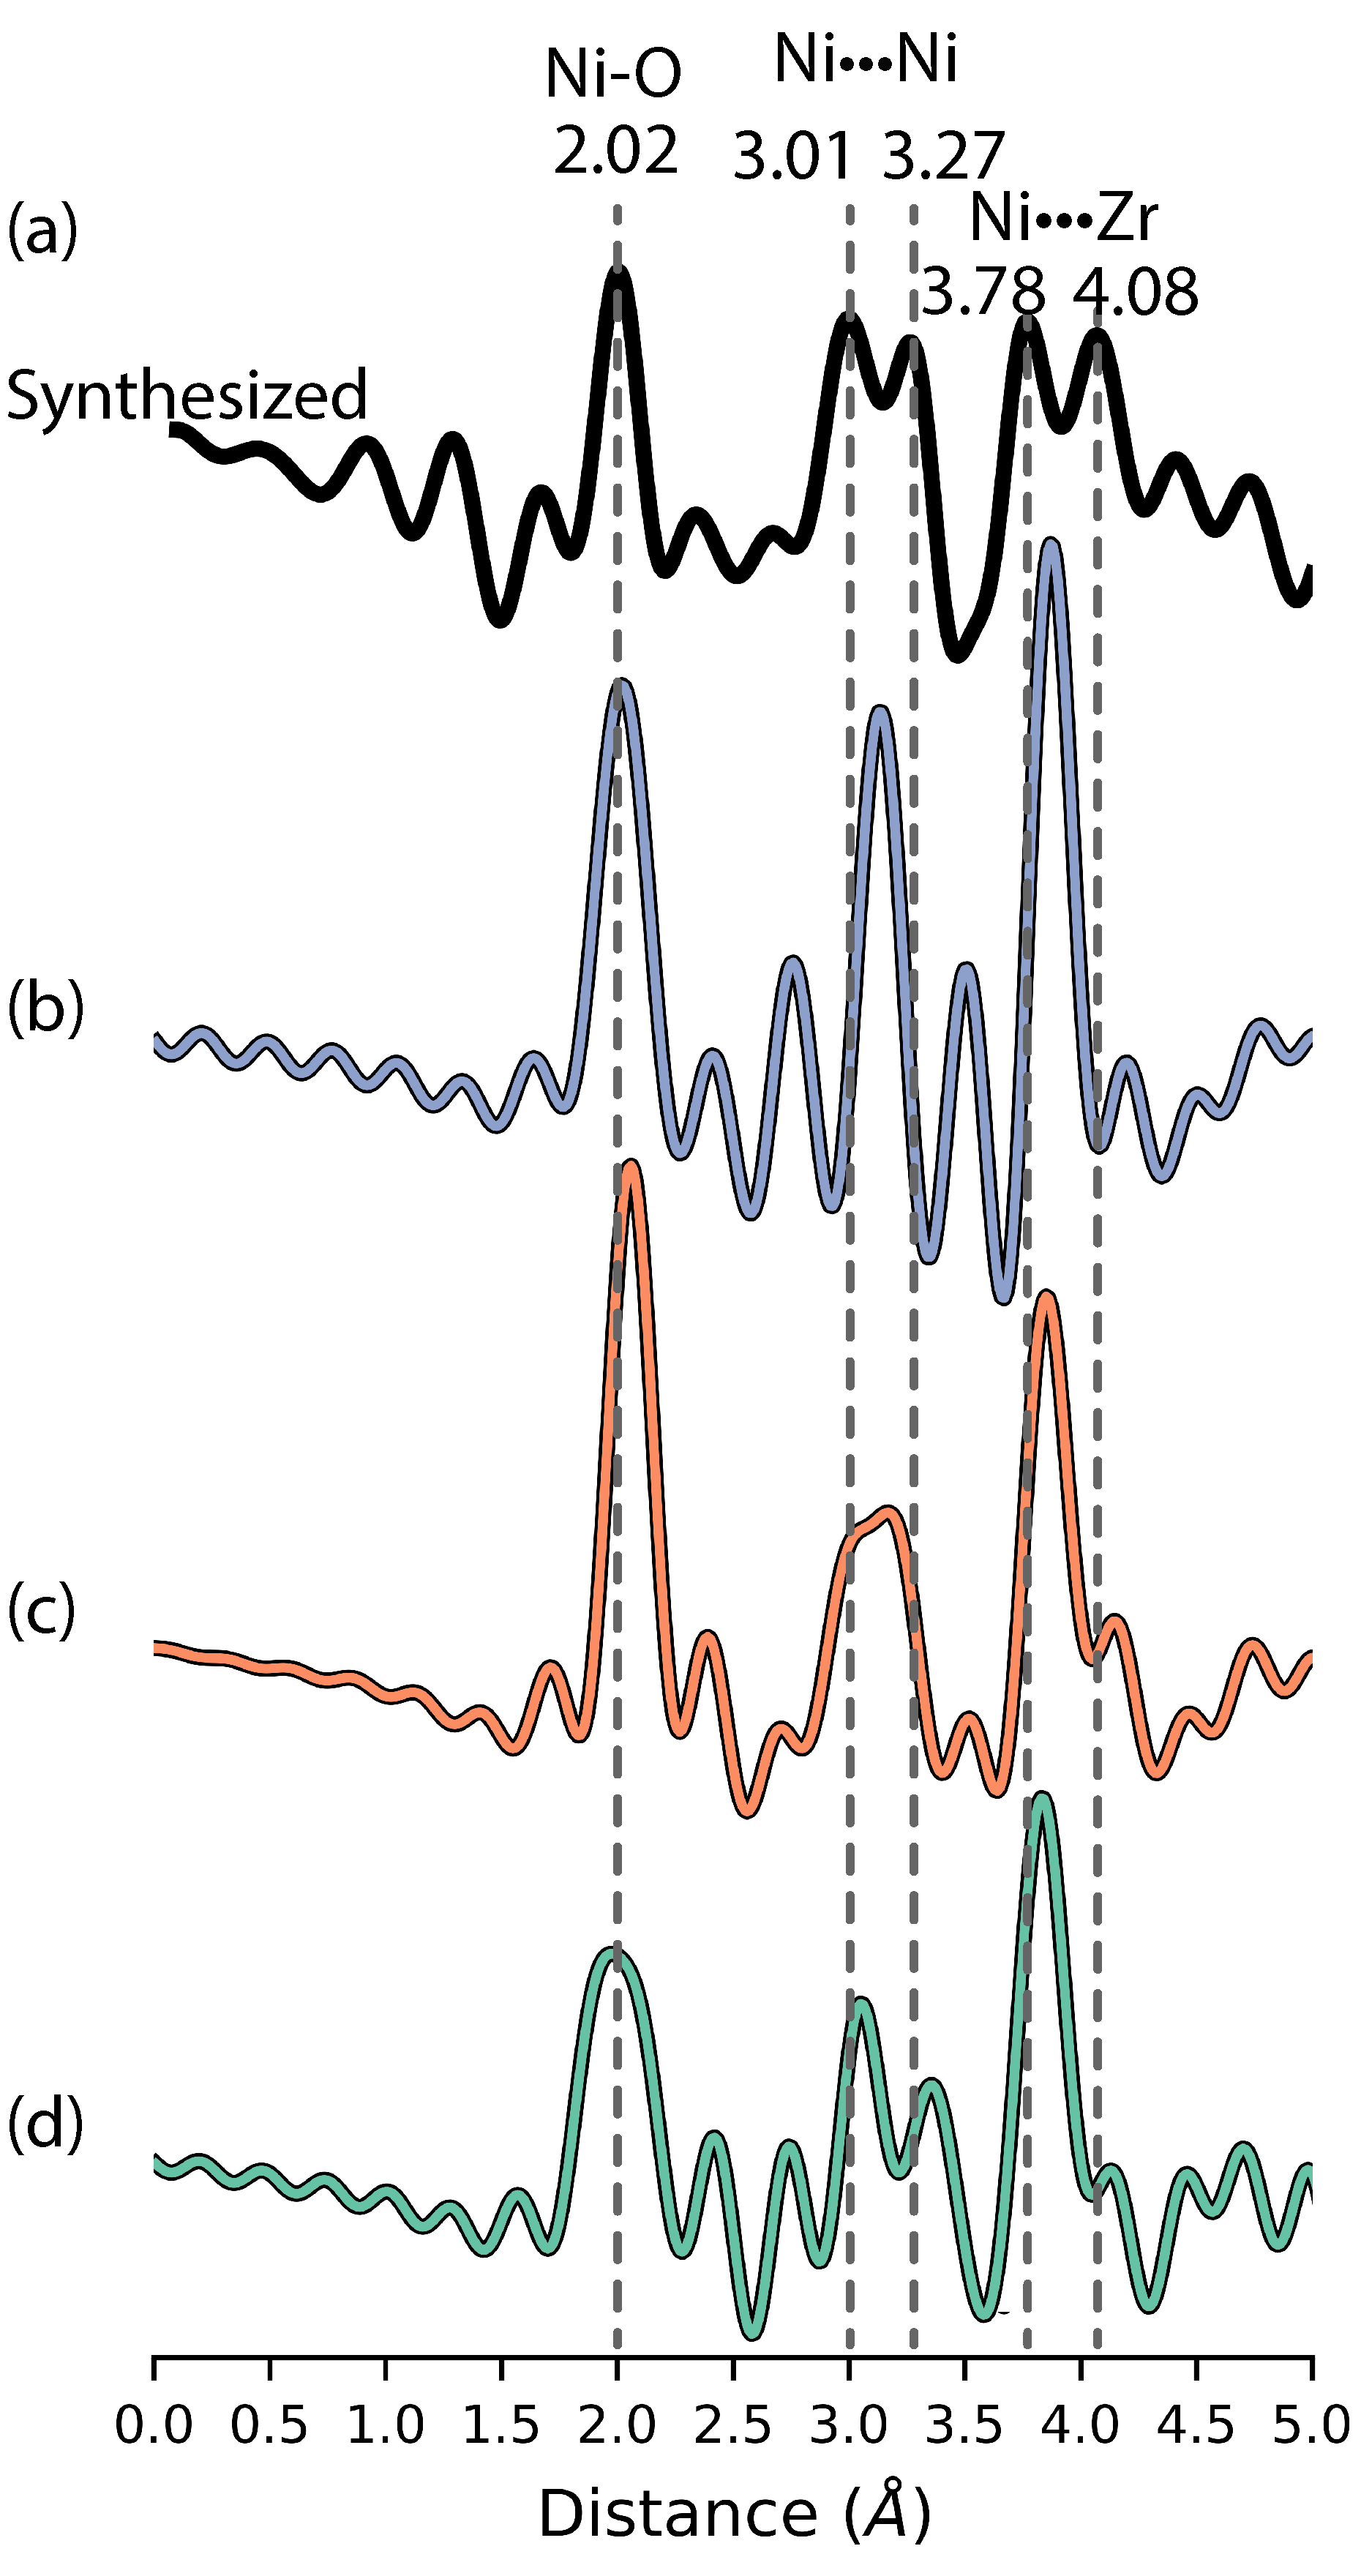
\includegraphics[width=0.50\textwidth]{zi-images/04-SI-images/2022-single-weighted_dPDF.png}
    \caption{
    The d-PDFs for (a) the synthesized structure and Botlzmann weighted d-PDFs (b-d). The Botlzmann weighted d-PDFs are determined at (b) $\mu_{\ce{H2O}}=$ -75.0 kJ/mol and $\mu_{\ce{H2}}=$ -200.0 kJ/mol, (c) $\mu_{\ce{H2O}}=$ 206.1 kJ/mol and $\mu_{\ce{H2}}=$ -250.0 kJ/mol, and (d) $\mu_{\ce{H2O}}=$ 206.1 kJ/mol and $\mu_{\ce{H2}}=$ -47.5 kJ/mol. Gray dotted lines indicate key distances observed for the synthesized structure, which are also annotated on the figure.
    }
    \label{fig:SI-weighted-dPDFs}
\end{figure}

%%%%%%%%%%%%%%%%%%%%%%%%%%%%%%%%%%%%%%%%%%%%%%%%%%%%%%%%%%%%%%%%%%%%%
%% Structure Heat Maps
%%%%%%%%%%%%%%%%%%%%%%%%%%%%%%%%%%%%%%%%%%%%%%%%%%%%%%%%%%%%%%%%%%%%%
\newpage
\section{Phase Diagram Structure Heat Maps}
We generate heat maps further probe the potential energy surface of the \ce{Ni4} cluster, and consider the sensitivity of the different regions appearing on the phase diagram. The heat maps are created by taking the difference in free energy values (denoted $\Delta \Delta F^{(2)}$) between structure ($i$) and the low energy structure ($o$) at $\Delta \mu_{\ce{H2O}}$ and $\Delta \mu_{\ce{H2}}$ (shown in Eq.~\ref{eq:delta_delta_F}). The low energy structure is the structure that is the thermodynamic minima at specific $\mu_{\ce{H2O}}$ and $\mu_{\ce{H2}}$ values. 
\begin{equation}
    \Delta \Delta F^{(2)}_{i}(V,T,\mu_{\text{H}}, \mu_{\text{O}}, N_{\text{Ni}}) = F^{(2)}_{i}(V,T,\mu_{\text{H}}, \mu_{\text{O}}, N_{\text{Ni}}) - F^{(2)}_{o}(V,T,\mu_{\text{H}}, \mu_{\text{O}}, N_{\text{Ni}})
    \label{eq:delta_delta_F}
\end{equation}
The heat maps for all thermodynamically relevant structures and select structures are shown in Figures~\ref{fig:SI-heatmap-combined} and~\ref{fig:SI-heatmap-combined_select}. 

\begin{figure}[H]
    \centering
    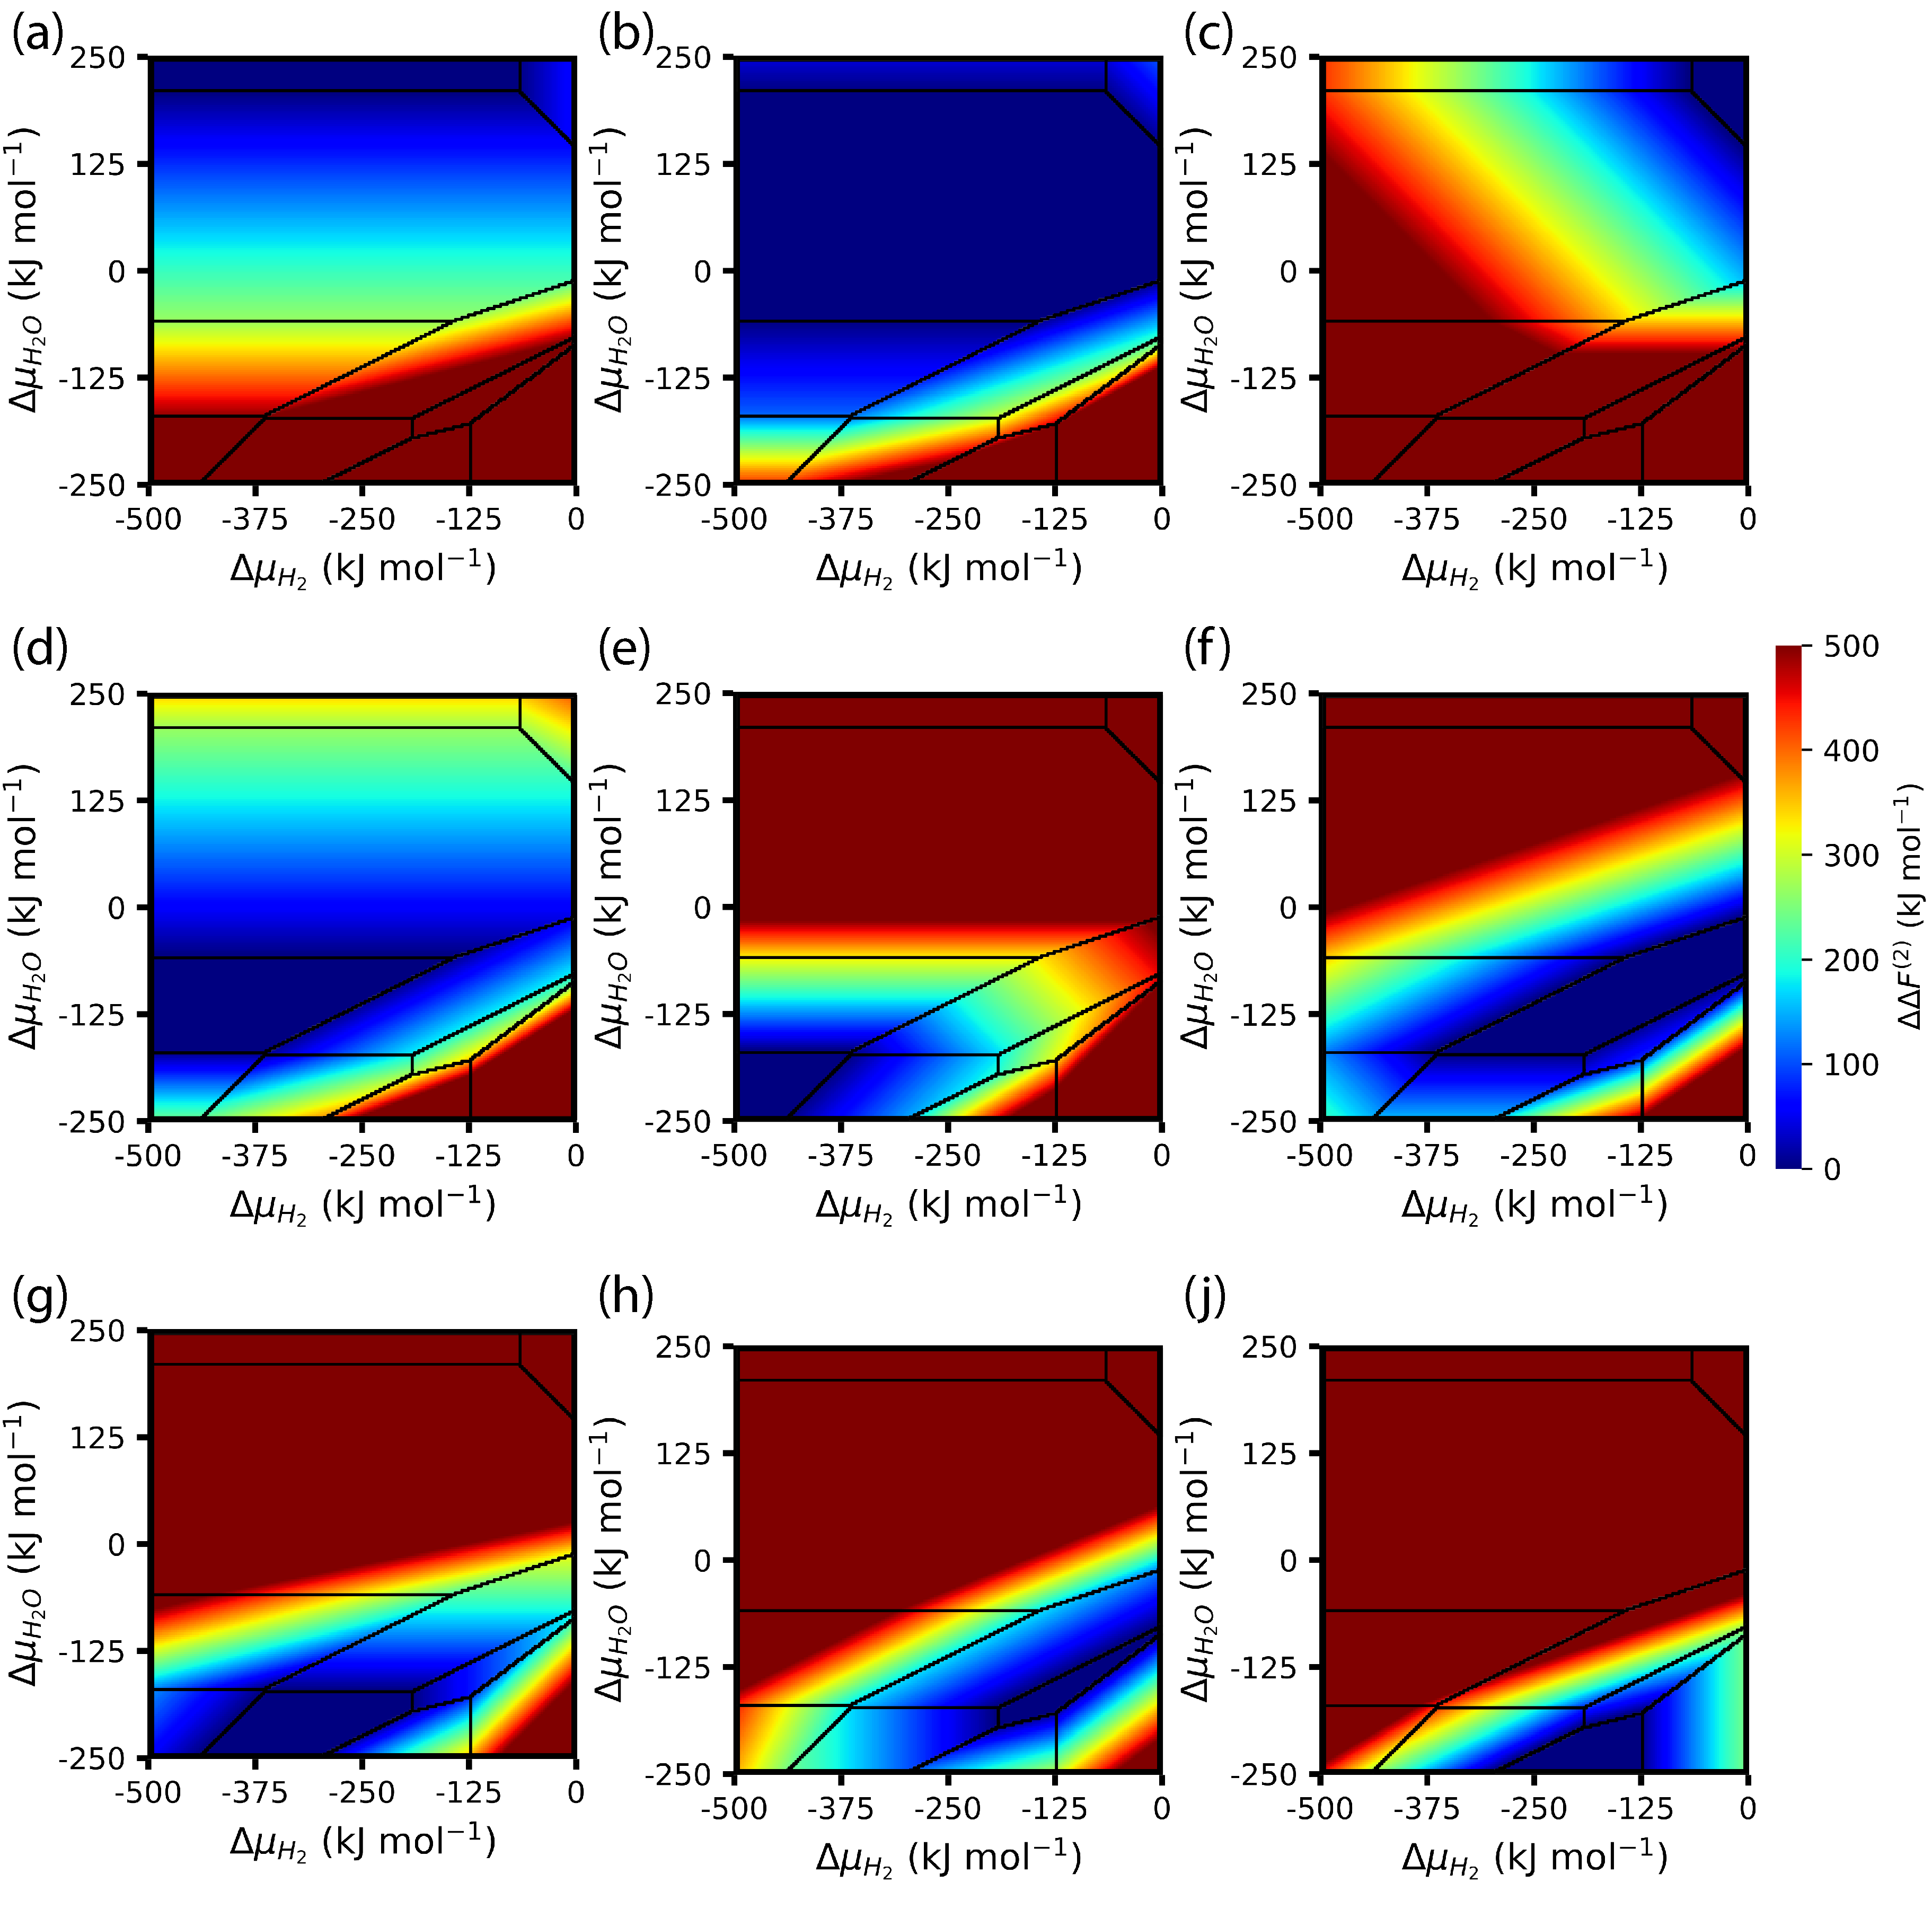
\includegraphics[width=0.95\textwidth]{zi-images/04-SI-images/SI-heat_map_combined.png}
    \caption{
        Heat map for the thermodynamic minima appearing on the phase diagram, which shows $\Delta \Delta F^{(2)}$ as a function of $\Delta \mu_{\ce{H2O}}$ and $\Delta \mu_{\ce{H2}}$. The following structure are shown: 
            (a) \ce{Ni4(OH)6.4H2O} (green)
            (b) \ce{Ni4(OH)6.3H2O} (purple)
            (c) \ce{Ni4(OH)5(H).4H2O} (blue)
            (d) \ce{Ni4(OH)6.2H2O} (cyan)
            (e) \ce{Ni4(OH)4(O)} (yellow)
            (f) \ce{Ni4(OH)4.2H2O} (orange)
            (g) \ce{Ni4(OH)4} (white)
            (h) \ce{Ni4(OH)3(H).H2O} (magenta)
            (j) \ce{Ni4} (gray)
    }
    \label{fig:SI-heatmap-combined}
\end{figure}

\begin{figure}[H]
    \centering
    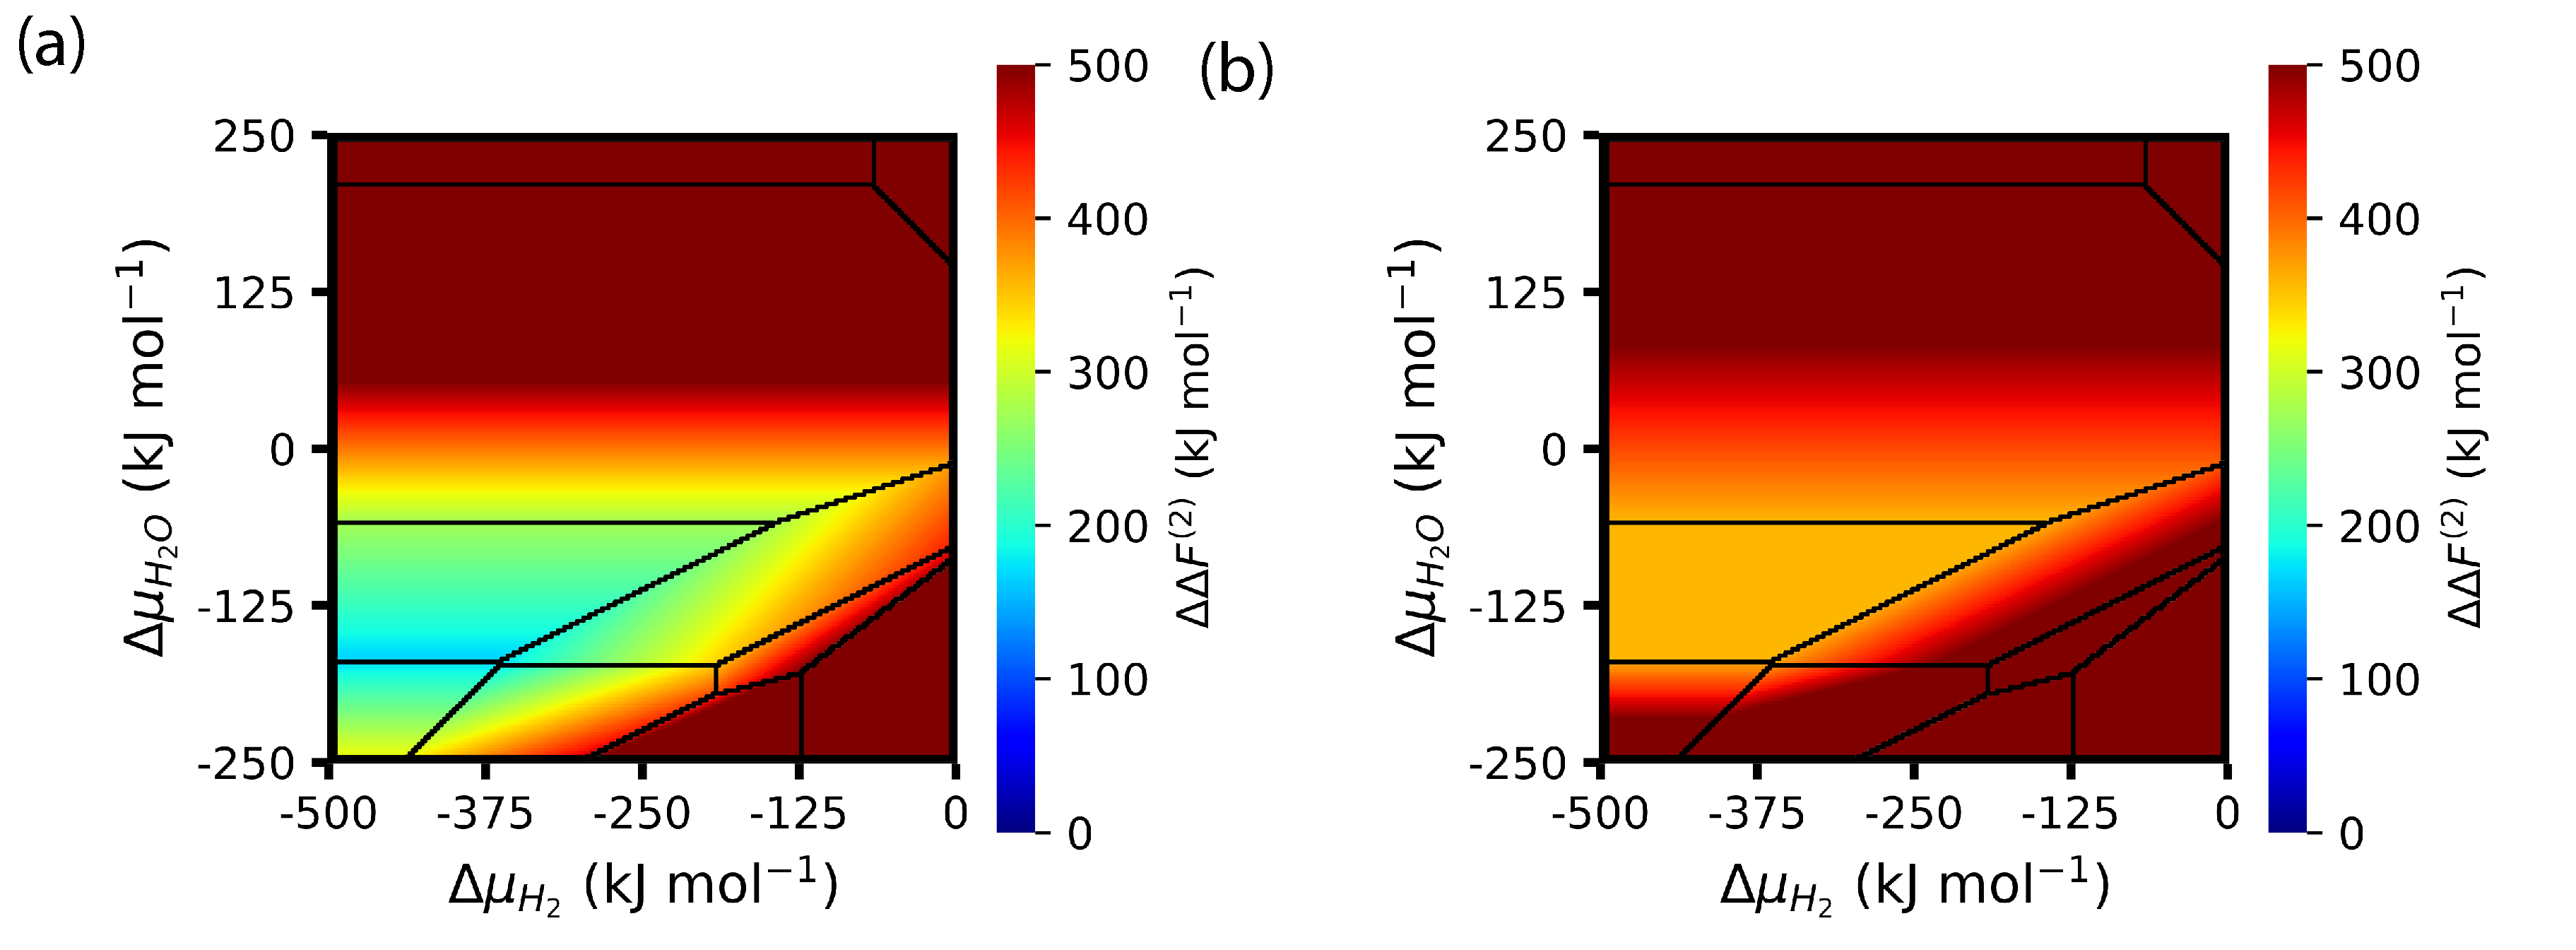
\includegraphics[width=0.95\textwidth]{zi-images/04-SI-images/SI-heat_map_combined_select.png}
    \caption{
        Heat map for the (a) \ce{Ni4(OH)6.1H2O} (teal) and (b) \ce{Ni4(OH)4(O).3H2O} (maroon) showing $\Delta \Delta F^{(2)}$ as a function of $\Delta \mu_{\ce{H2O}}$ and $\Delta \mu_{\ce{H2}}$. Both structures are not thermodynamic minima under any of the explored conditions, as shown by the heat maps. 
    }
    \label{fig:SI-heatmap-combined_select}
\end{figure}

%%%%%%%%%%%%%%%%%%%%%%%%%%%%%%%%%%%%%%%%%%%%%%%%%%%%%%%%%%%%%%%%%%%%%
%% The appropriate \bibliography command should be placed here.
%% Notice that the class file automatically sets \bibliographystyle
%% and also names the section correctly.
%%%%%%%%%%%%%%%%%%%%%%%%%%%%%%%%%%%%%%%%%%%%%%%%%%%%%%%%%%%%%%%%%%%%%
\newpage
\bibliography{achemso-demo}

\end{document}